%
%
% you should only have one "documentclass" line.  the following lines
% are samples that give various options.  the nofrontmatter option is
% nice because it suppresses the title and signature pages when you want
% to focus only on the main body of the thesis
%
% Friday April 10 2010 Ray Hylock <ray-hylock@uiowa.edu>
% documentclass options:
%   docabstract				if you want to add a separate doctoral abstract with separate signature page
%   abstractpage            if you want to add an internal abstract (optional)
%	publicabstractpage		if you want to add a public abstract page 
%   ackpage                 if you would like to add an acknowledgements page (optional)
%   algorithms              if you want a list of algorithms (optional)
%   appendix                if you have an appendix (optional)
%   copyrightpage           if you wish to copyright your thesis (optional)
%   dedicationpage          if you wish to make a dedication (optional)
%   epigraphpage            if you would like to add an epigraph to the beginning of your thesis (optional)
%   examples                if you want a list of examples (this uses the ntheorem package)
%   exampleslemmas          if you want a combined list of examples and lemmas (this uses the ntheorem package) (optional)
%   examplestheorems        if you want a combined list of examples and theorems (this uses the ntheorem package) (optional)
%   exampleslemmastheorems  if you want a combined list of examples, lemmas, and theorems (this uses the ntheorem package) (optional)
%   figures                 if you have any figures (this is required if you have even one figure)
%   lemmas                  if you want a list of lemmas (this uses the ntheorem package) (optional)
%   lemmastheorems          ifs you want a combined list of lemmas and theorems (this uses the ntheorem package) (optional)
%   nofrontmatter           suppresses the title and signiture pages for working on the body
%   tables                  if you have any tables (this is required if you have even one table)
%   theorems                if you want a list of theorems (this uses the ntheorem package) (optional)
%   phd                     if phd student; this will add the doctoral abstract (mandatory for PhD and DMA thesis candidates only)
%
\documentclass[abstractpage,publicabstractpage,ackpage,copyrightpage,phd,figures,tables]{uithesis}
\usepackage{amsfonts}
\usepackage{amsmath}
\usepackage{amssymb}
\usepackage{amsthm} % included in ntheorem with amsthm option
%\usepackage[amsthm]{ntheorem} % use if going to make theorem lists
\usepackage{array}
\usepackage{float}
\usepackage[toc,page,titletoc]{appendix}
\usepackage{longtable}
\usepackage{graphicx}
\usepackage[font=singlespacing]{caption}
\usepackage[normalem]{ulem}
\usepackage{nicefrac}
\usepackage{units}
\usepackage{rotating}
\usepackage{afterpage}
\usepackage{tikz}
\usetikzlibrary{arrows,positioning}
\usepackage{tikz-cd}
\usepackage{subcaption}
\usepackage[hidelinks]{hyperref}
\usepackage{cleveref}
\usepackage{multirow}
\usepackage{rotating}
\usepackage{makecell}
\usepackage{rotating}
%\usepackage[nottoc,notlot,notlof]{tocbibind}

\usepackage{listings}
\usepackage{xcolor}
\definecolor{codegreen}{rgb}{0,0.6,0}
\definecolor{codegray}{rgb}{0.5,0.5,0.5}
\definecolor{codepurple}{rgb}{0.58,0,0.82}
\definecolor{backcolour}{rgb}{0.96,0.96,0.93}

\lstdefinestyle{mystyle}{
escapeinside={(*@}{@*)},
backgroundcolor=\color{backcolour},
commentstyle=\color{codepurple},
keywordstyle=\color{blue},
emphstyle=\color{red},
numberstyle=\tiny\color{codegray},
stringstyle=\color{codegreen},
basicstyle=\ttfamily\footnotesize,
breakatwhitespace=false,
breaklines=true,
captionpos=b,
keepspaces=true,
numbers=left,
numbersep=5pt,
showspaces=false,
showstringspaces=false,
showtabs=false,
tabsize=2,
language=R,
keywords={},
otherkeywords={build\_vae\_independent, build\_vae\_correlated, train\_model, get\_item\_parameter\_estimates, get\_ability\_parameter\_estimates, responses, q\_matrix, correlation\_matrix, disc\_true, diff\_true, theta\_true}
}
\lstset{style=mystyle}

% compress and sort citations as numbers
% alter uithesis.cls line 355 from plain2 to unsrt to use this
%\usepackage[numbers,sort&compress]{natbib}

% does not allow citations to be split between pages; requirement
\usepackage{etoolbox}
\apptocmd{\thebibliography}{\interlinepenalty 10000\relax}{}{}

% Vertical spacing (singlespace) in itemset and enumerate
\usepackage{enumitem}
\setlist{noitemsep,topsep=1pt, partopsep=4pt, parsep=2pt}
\setenumerate{noitemsep,topsep=1pt, partopsep=4pt, parsep=2pt}

% single spacing for rows in a table (this does not single space
% within a row; for that, use \\[-5mm]
\renewcommand\arraystretch{0.5} % 1/2 of the default spacing (double)

\allowdisplaybreaks[2]

% Put user defined commands here
% The \sideremark command is very useful for margin comments

\newcommand{\be}{\begin{enumerate}}
\newcommand{\ee}{\end{enumerate}}

\newtheorem{theorem}{Theorem}[chapter]
\newtheorem{lemma}[theorem]{Lemma}
\newtheorem{corollary}[theorem]{Corollary}
\newtheorem{proposition}[theorem]{Proposition}
\newtheorem{example}[theorem]{Example}
%% math commands
\def \R{\ensuremath \mathbb{R}}
\def \e{\ensuremath \varepsilon}
\def \d{\ensuremath \delta}
\def \tr{\ensuremath \text{tr}}
\newcommand{\vect}[1]{\boldsymbol{#1}}

\theoremstyle{definition}
\newtheorem{defn}[theorem]{Definition}
\newtheorem{remarkalgorithm}[theorem]{Algorithm}
\newtheorem{hypothesis}[theorem]{Hypothesis}

\theoremstyle{remark}
\newtheorem{remark}[theorem]{Remark}

\pdfstringdefDisableCommands{\let\uppercase\relax}

% For figures
\newcommand*{\figuretitle}[1]{
  {\centering
  \textbf{#1}
  \par\medskip}
}
\newcommand*{\figuretitlesmall}[1]{
  {\centering \scriptsize{
  \textbf{#1}
  \par\medskip}}
}


%
% the following command can be used to put a remark
% in the margin of the thesis/paper
% to include a remark, use \edz{remark}
% size of the remark font can be changed, not it
% is set to "scriptsize", can also be "tiny" or "small"
% or others
%
\def\sideremark#1
{
\ifvmode\leavevmode\fi\vadjust
  {\vbox to0pt
    {\vss\hbox to0pt
      {\hskip\hsize\hskip1em\vbox
        {\hsize2cm
%          \small
          \scriptsize
          \raggedright\pretolerance10000\noindent#1\hfill
        }
        \hss
      }
      \vbox to8pt{\vfil}\vss
    }
  }
}


% !Tex root = thesis.tex

% This is the prelude to my thesis and contains much of what is needed to
% create my thesis


%% Front Matter %%%%%%%%%%%%%%%%%%%%%%%%%%%%%%%%%%%%%%%%%%%%%%%%%%%%%%%%
%\abtitlepgfalse       % print out the microfiche title page
%\abstractpgfalse      % print out the microfiche abstract
% \abtitlepgtrue       % print out the microfiche title page
% \abstractpgtrue      % print out the microfiche abstract

%\titlepgtrue          % print out the title page
%\copyrightfalse       % claim my true inheritance
%\signaturepagetrue    % page for thesis committee members
%\dedicationtrue       % page for the dedication
%\acktrue              % Print out the acknowledgements
%\abswithesisfalse     % abstract for the thesis
%\tablecontentstrue    % page for table of contents
%\figurespagefalse     % page of figures
%%%%%%%%%%%%%%%%%%%%%%%%%%%%%%%%%%%%%%%%%%%%%%%%%%%%%%%%%%%%%%%%%%%%%%%%%

%%%%% TITLE %%%%%%%%%%%%
\title{Geoff's Thesis}

%%%%%%%%% AUTHOR %%%%%%%%%%%%
\author{Geoffrey Converse}
%%%%%%%%% Other Stuff %%%%%%%%%%%%
\dept{Applied Mathematical and Computational Sciences}
% for a single advisor
\setboolean{multipleSupervisors}{false}
\advisor{Professor Suely Oliveira} %  \hspace{56mm} Second Advisor Title and Name}
% for multiple advisors; change <value> to line up the names
%\setboolean{multipleSupervisors}{true}
%\advisor{Advisor 1\\\hspace{4mm}Advisor 2...}
%
% edit the names below to have your committee members names appear
% on the signature page.  memberOne should be your advisor.
%
\memberOne{Professor Suely Oliveira}
\memberTwo{Member Two}
\memberThree{Member Three}
\memberFour{Member Four}
\memberFive{Member Five}
% Comment in if there are six committee members, also need to comment in two commands in thesis.cls, search "six committee members" to find where to comment in commands in thesis.cls
%\memberSix{Member Six}

\submitdate{Date?}
\copyrightyear{2021}


% Abstracts for the various purposes
%\newcommand{\abstextwithesis}{\myabstract}
%\newcommand{\abstracttext}{\myabstract}

% Dedication for the thesis.
\epigraph{epigraph}
\dedication{dedication}

% Acknowledgement file
\ackfile{thesisAck}
% Abstract file - specifies the text for the abstract.  This is used
% in the PhD Abstract, as well as in the abstract bounded with
% the dissertation
\abstractfile{thesisAbstract}
\publicabstractfile{thesisAbstractpublic}


       % Front matter, title page, etc.

\begin{document}

% Puts some of the front matter in
\frontmatter

% Include the chapters and appendix here

\chapter{Introduction}
TODO: I should have an introduction to the full work here.

\section{Organization}
This thesis is organized in three parts. In Part I, the first three chapters introduce Item Response Theory (IRT) and analyzes the novel parameter estimation method, ML2P-VAE. This method uses a modified variational autoencoder to estimation parameters in IRT models. Chapters 5-7 of Part II explore a task commonly seen in electronic learning environments in knowledge tracing. While other deep learning methods for knowledge tracing lack interpretability, new methods presented here present a trade-off between prediction power and explainability. Part III explores two applications of the ML2P-VAE method in areas outside of education: sports analytics and health sciences.

\sideremark{TODO: what is the best way to do this organization chapter?}



% Part I
\chapter{Item Response Theory Background} \label{ch:irt_background}

In educational measurement, a common goal is to quantify the knowledge of students from the results of some assessment. In a classroom setting, grades are typically assigned based on the percentage of questions answered correctly by a student assignments. The letter grades assigned from these percentages can serve as a naive measure of student knowledge; ``A'' students have completely mastered the material, ``B'' students have a good grasp of material, ``C'' students are fairly average, and ``D'' and ``F'' students have significant gaps in their knowledge.

The practice of evaluating student ability purely from a raw percentage score is known as true score theory \cite{thissen}. But there are clear issues with this approach. Not all questions on an exam or homework assignment is created equally: some questions are easier, and some more difficult. Consider a scenario where two students both answer 17 out of 20 questions correctly on a test for a raw score of $85\%$. But if Student A answered questions 1, 8, and 9 wrong while Student B answered 4, 17, and 20 incorrectly, it is not likely that that Student A and Student B possess the same level of knowledge. For example, questions 1, 8, and 9 could be much more difficult than questions 4, 17, and 20. Additionally, the two sets of problems could cover different types of material. True score theory does not account for either of these situations, and naively quantifies the knowledge of Student A and Student B as equal.

More sophisticated methods have been studied which attempt to more accurately quantify student learning. Cognitive Diagnostic Models (CDM) (TODO: citation) aim to classify whether students possess mastery of a given skill or not. This discrete classification can be useful in determining whether or not a student meets a prerequisite, or deciding whether or not they are ready to move on to the next level of coursework. We focus instead on Item Response Theory, where student knowledge is assumed to be continuous.

\section{Item Response Theory}
Item Response Theory (IRT) is a field of quantitative psychology which uses statistical models to model student ability \cite{lord1968}. These models often give the probability of a question being answered correctly as a function of the student's ability. In IRT, it is assumed that each student, indexed by $j$, possesses some continuous latent ability $\theta_j$. The term ``latent ability'' is synonymous with ``knowledge''or ``skill.'' Often, it is assumed that amongst the population of students, $\theta_j \sim \mathcal{N}(0,1)$ \cite{thissen}. 

In this work, we often consider the case where each student has multiple latent abilities. For example, in the context of an elementary math exam, we may wish to measure the four distinct skills ``add'', ``subtract'', ``multiply'', and ``divide.'' This scenario is referred to as multidimensional item response theory, and we write the set of student $j$'s $K$ latent abilities as a vector $\Theta_j = (\theta_{1j}, \theta_{2j}, \ldots, \theta_{Kj})^\top$. It is then assumed that the latent abilities of students follow some multivariate Gaussian distirbution, $\mathcal{N}(0, \Sigma)$. For simplicity, the covariance matrix $\Sigma$ is often taken to be the identity matrix, making each latent skill independent of one another.

Note that $\Theta_j$ is not directly observable in any way. Instead, a common goal is to infer student's knowledge $\Theta_j$ from on their responses on some assessment containing $n$ questions, referred to as items. A student's set of responses can be written as a binary $n$-dimensional vector $\vec u_j = (u_{1j}, u_{2j}, \ldots, u_{nj})^\top$, where 
\begin{equation}
  u_{ij} = \begin{cases} 1 & \text{if student } j \text{ answers item } i \text{ correctly} \\0 & \text{otherwise} \end{cases} 
  \label{eq:responses}
\end{equation}
IRT models aim to model the probability of a student answering a particular question correctly, so that the probability of student $j$ answering item $i$ correctly is given by some function of $\Theta_j$:
\begin{equation}
  P(u_{ij} = 1 | \Theta_j) = f(\Theta_j; V_i)
\end{equation}
where $V_i$ is a set of parameters associated with item $i$. In general, $f:\R^K \to [0,1]$ is some continuous function which is strictly increasing with respect to $\Theta_j$.

\begin{figure}[h]
  \centering
  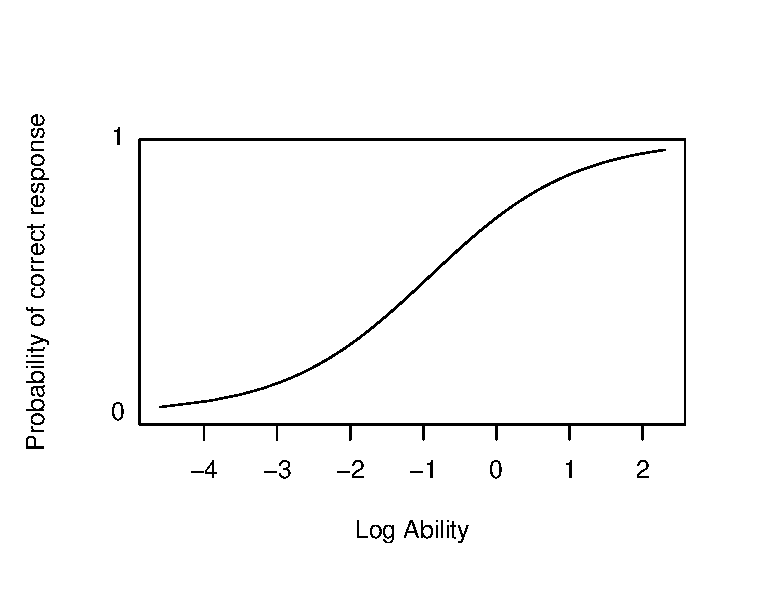
\includegraphics[width=.6\textwidth, angle=90]{img/logistic_1param_icc.eps}
  \caption{An item characteristic curve visualizes the relation between a student's ability and the probability of answering an item correctly.}
  \label{fig:icc}
\end{figure}

In the following sections, we describe various candidates for the function $f$. Though each is presented in the context of single-dimensional IRT ($K = 1$), they can all be easily adapted to higher dimensions.

\subsection{Rasch Model}
One of the first models was proposed by Georg Rasch in 1960. Rasch asserted that the probability of a student answering an item correctly is a function of the ratio $\xi / \d$, where $\xi > 0$ represents the student's knowledge, and $\d > 0$ quantifies the difficulty of an item. Consider the $\frac{\xi}{\xi + \d} = \frac{1}{1 + \d / \xi}$ and note that $\frac{\xi}{\xi + \d} \to 1$ as $\xi \to \infty$. After the reparametarization $\xi = e^{\theta}$ and $\d = e^{b}$, we arrive at the 1-Parameter Logistic Model, often referred to as the Rasch Model.
\begin{equation}
  P(u_{ij} = 1 | \theta_j; b_i) = \frac{1}{1 + e^{b_i - \theta_j}}
  \label{eq:1pl}
\end{equation}

Note that $\theta \in \R$ and $b \in \R$ still represent student ability and item difficulty, respectively. We can interpret the difficulty parameter $b$ as a threshold: when $\theta = b$, then the student has a $50\%$ chance of answering the question correctly. A plot of Equation \ref{eq:1pl} for a fixed item (fixed $b_i$) is shown in Figure \ref{fig:icc}. The horizontal axis represents $\log \theta$, and the vertical axis represents $P(u_{ij} = 1 | \theta, b_i)$. This type of graph is often referred to as an item characteristic curve (ICC).

\subsection{Normal Ogive Model}
\sideremark{*This section isn't very important to rest of work}
A slightly more sophisticated method for measuring student performance is the normal ogive model. We introduce a discrimination parameter, $a_i$, which quantifies the capability of item $i$ in distinguishing between students who have / have not mastered the knowledge concept $\theta$ \cite{thissen}. In other words, $a_i$ tells \textit{how much} of skill $\theta$ is required to answer item $i$ correctly. 

The normal ogive model give the probability of student $j$ answering item $i$ correctly as
\begin{equation}
  P(u_{ij} = 1 | \theta_j; a_i, b_i) = \frac{1}{\sqrt{2\pi}} \int_{-a_i \theta_j + b_i}^\infty e^{\frac{-z^{2}}{2}}dz
  \label{eq:ogive}
\end{equation}
Note the similarity between Equation \ref{eq:ogive} and the cumulative distribution function for a Gaussian distribution. The normal ogive model is popular among statisticians for this reason, but can be difficult to use for parameter estimation. 

\subsection{2-Parameter Logistic Model}
The model which this work focuses on most is the 2-parameter logistic (2PL) model. Like the normal ogive model, the 2PL model uses both the discrimination and difficulty item parameters. The probability of student $j$ answering item $i$ correctly is given by
\begin{equation}
  P(u_{ij} = 1 | \theta_j; a_i, b_i) = \frac{1}{1 + e^{-a_i \theta_j + b_i}}
  \label{eq:2PL}
\end{equation}
Equation \ref{eq:2PL} has the same form as that of the Rasch model in Equation \ref{eq:1pl}, but adds in the discrimination parameter $a_i$. If this parameter is scaled by 1.7, then the ICC from the normal ogive model differs from that of the 2PL model by $0.01$ \cite{baker_kim2004}. In a sense, we can consider the 2PL model to be a very good approximation of the normal ogive model. Due to the simple form of Equation \ref{eq:2PL}, using this model makes parameter estimation much easier.

\subsection{Multidimensional Item Response Theory}
The previously described statistical models can all be extended so that each student possesses $K$ latent traits. In multidimensional item response theory (MIRT), models give the probability of a correct answer as a function of the student ability vector $\Theta = (\theta_1,\ldots, \theta_K)^\top$. The generalization of \ref{eq:2PL} is given by the multidimensional logistic 2-parameter (ML2P) model:
\begin{equation}
P(u_{ij} = 1 | \Theta_j; \vec{a_i}, b_i) = \frac{1}{1 + \exp\left(-\vec{a_i}^\top \Theta_j + b_i\right)} = \frac{1}{\exp\left(-\sum_{k=1}^K a_{ik} \theta_{kj} + b_i \right)}
  \label{eq:ml2p}
\end{equation}
Here, the discrimination parameters $\vec{a_i} \in \R^K$ are given as vector, where each entry $a_{ik} \in \vec{a_i}$ quantifies \textit{how much} of skill $k$ is required to answer item $i$ correctly. The ML2P model is the main focus of this thesis.

TODO: mention MDISC and how this scales

In MIRT, it is convenient to notate the relationship between skills and items with binary matrix. Define the $Q$-matrix \cite{daSilva2018} $Q \in \{0,1\}^{n\times K}$ so that 
\begin{equation}
  q_{ik} = \begin{cases}
    1 & \text{if item } i \text{ requires skill } k\\
    0 & \text{otherwise}
  \end{cases}.
  \label{eq:q_matrix}
\end{equation}
In real applications, the $Q$-matrix is annotated by an expert in the field, as it is usually possible to discern the concepts need to answer an item correctly. In relation to the ML2P model (Equation \ref{eq:ml2p}), notice that if $q_{ik} = 0$, then $a_{ik} = 0$ as well. Though experts can produce a $Q$-matrix for a given assessment, the matrix of discrimination parameters $(a_{ik})_{i,k}$ can not be discovered so easily.

\section{IRT Parameter Estimation}
\sideremark{*How in-depth do these descriptions need to be? Could just give overall idea and describe weaknesses}

\subsection{Maximum Likelihood Estimation}
TODO: item parameter estimation

TODO: ability parameter estimation

\subsection{Joint Maximum Likelihood Estimation}


\subsection{Marginal Maximum Likelihood Estimation}
TODO: MMLE

TODO: EM 

\section{Artificial Neural Networks}
In recent years, artifical neural networks (ANN) have become an increasingly popular tool for machine learning problems. Though they have been around since the 1960's (TODO: citation), GPU technology has become more accessible and modern computers are more powerful, allowing anyone interested to train a basic neural network on their machine. ANN can be applied to a diverse set of problems, including regression, classification, computer vision, natural language processing, function approximation, data generation, and more (TODO: citations).

One of the biggest critiques of ANN is their black-box nature, meaning that the decision process that a trained model uses is typically not explainable by humans. As opposed to simpler methods such as decision trees or linear regression, neural networks are not interpretable. This makes them less desirable in certain applications where researchers wish to know \textit{why} a model predicts a particular data sample the way that it does. For example, if a financial institution is using data science methods to determine whether or not to approve someone's loan, the institution should be able to explain to the customer why they were denied. Most customers will not be satisfied with ``the computer told us so,'' and there is a possibility that a black-box neural network could learn and use features such as race or gender in its prediction, which is illegal in the United States (TODO: definitely need citation or delete).

The push for explainable AI have led researchers down two paths. One group has tried to incorporate deep learning methods with existing interpretable methods, in hopes of increasing the performance of explainable methods without sacrificing its interpretability (TODO: citation). Another option is to use a sort of hybrid learning, where interpretable models defer to a black-box model if they are not confident in their prediction \cite{rafique2020}. Others have started with deep models and cut back on complexity, making specific modifications which increase interpretability. For example, the loss function of a convolutional neural network can be adapted so that humans can understand the features extracted in the hidden layers \cite{zhang2018interpretable}. 

The field of education is an application which often desires interpretable models. Researchers often need to be able to point out specific details of decisions made by AI. A student deserves an answer to \textit{why} they failed a test, and a teacher should be given instructions on \textit{how} to fix the student's misconceptions.

\subsection{Autoencoders}
An autoencoder (AE) is a neural network where the input and output layers are the same shape. The objective for a given data point is to minimize the difference between the output, called the reconstruction, and the input. Typically, the middle hidden layers of an AE are of smaller dimension than the input space. In this way, autoencoders are an unsupervised learning technique for (nonlinear) dimension reduction. Mathematically, we can define an autoencoder in two parts as follows.

For an input $x \in \R^n$, define the \textit{encoder} as a function $f: \R^n \to \R^m$ mapping $x \mapsto z := f(x)$. Usually, $m < n$, and $z$ lies in a hidden feature space. The encoder sends an observed data point to its representation in a learned feature space. Define the \textit{decoder} as a function $g: \R^m \to \R^n$ mapping $z \mapsto \hat x := g(z)$. The decoder maps a hidden representation $z$ to a reconstruction of the encoder input. Note that in our case, the functions $f$ and $g$ are both parameterized by neural networks, each of which can have any number of hidden layers. The end-to-end autoencoder is then the function composition $\mathcal{A}(x):= g(f(x)): \R^n \to \R^n$. To train an AE, the loss function minimizes the difference between the input and output. This can be done in a number of ways, including the simple mean squared error loss
\begin{equation}
  \mathcal{L}(x) = || x - g(f(x))||_2^2
  \label{eq:mse}
\end{equation}
or cross-entropy loss for binary data
\begin{equation}
  \mathcal{L}(x) = \sum_{i=1}^n - x_i \log(g(f(x_i))) - (1-x_i)\log(1- g(f(x_i))).
  \label{eq:cross_entropy}
\end{equation}

Autoencoders with only a single hidden layer can be compared with nonlinear principal components analysis (PCA), and using linear activation functions allows for recovery of PCA loading vectors \cite{plaut2018}. AEs have clear applications in image compression straight out-of-the-box, and can be modified for more complicated problems. Denoising autoencoders \cite{vincent2008} are capable of processing noisy images and cleaning them up. To do this, they corrupt input data by deleting pixels at random and reconstructing the original image. Autoencoders can also be modified for data generation applications using a variational autoencoder.

\subsection{Variational Autoencoders}
*relevant sources: \cite{doersch2016} \cite{kingma2014} \cite{Blei2017}, infoVAE, ELBO, ``towards deeper understanding of VAE''

TODO: describe probabilistic derivation of VAE (ie Kingma and Welling). Also talk about how Zhao et al (InfoVAE) show that if decoder is Gaussian, then maximizing ELBO makes the latent distribution bad - but I've shown this isn't the case in our model, where the decoder is Bernoulli.


%\chapter{Survey of Relevant Neural Networks}

In recent years, artificial neural networks (ANN) have become an increasingly popular tool for machine learning problems. Though they have been around since the 1960's \cite{rosenblatt1961}, GPU technology has become more accessible and modern computers are more powerful, allowing anyone interested to train a basic neural network on their machine. ANN can be applied to a diverse set of problems, including regression, classification, computer vision, natural language processing, function approximation, data generation, and more \cite{hammerstrom1993} \cite{zhang2000}.

One of the biggest critiques of ANN is their black-box nature, meaning that the decision process that a trained model uses is typically not explainable by humans. As opposed to simpler methods such as decision trees or linear regression, neural networks are not interpretable. This makes them less desirable in certain applications where researchers wish to know \textit{why} a model predicts a particular data sample the way that it does. For example, if a financial institution is using data-driven methods to determine whether or not to approve someone's loan, the institution should be able to explain to the customer why they were denied. Most customers will not be satisfied with ``the computer told us so,'' and it is possible that a black-box neural network could learn and use sensitive information such as race, age, or gender in its prediction, which would raise legal questions in the United States \cite{ecoa}.

The push for explainable AI has led to multiple approaches to increase model interpretability. Some have aimed to incorporate deep learning methods with existing interpretable methods, in hopes of increasing the performance of explainable methods without sacrificing its interpretability \cite{goebel2018}. Another option is to use a sort of hybrid learning, where interpretable models defer to a black-box model if they are not confident in their prediction \cite{rafique2020}. Others have started with deep models and cut back on complexity, making specific modifications which increase interpretability. For example, the loss function of a convolutional neural network can be adapted so that humans can understand the features extracted in the hidden layers \cite{zhang2018interpretable}. 

The field of education is an application which often desires interpretable models. Researchers often need to be able to point out specific details of decisions made by AI. A student deserves an answer to \textit{why} they failed a test, and a teacher should be given instructions on \textit{how} to fix the student's misconceptions.

\section{Autoencoders}
An autoencoder (AE) is a neural network where the input and output layers are the same shape. The objective for a given data point is to minimize the difference between the output, called the reconstruction, and the input. Typically, the middle hidden layers of an AE are of smaller dimension than the input space. In this way, autoencoders are an unsupervised learning technique for (nonlinear) dimension reduction. Mathematically, we can define an autoencoder in two parts as follows.

For an input $x \in \R^n$, define the \textit{encoder} as a function $f: \R^n \to \R^m$ mapping $x \mapsto z := f(x)$. Usually, $m < n$, and $z$ lies in a hidden feature space. The encoder sends an observed data point to its representation in a learned feature space. Define the \textit{decoder} as a function $g: \R^m \to \R^n$ mapping $z \mapsto \hat x := g(z)$. The decoder maps a hidden representation $z$ to a reconstruction of the encoder input. Note that in our case, the functions $f$ and $g$ are both parameterized by neural networks, each of which can have any number of hidden layers. The end-to-end autoencoder is then the function composition $\mathcal{A}(x):= g(f(x)): \R^n \to \R^n$. To train an AE, the loss function minimizes the difference between the input and output. This can be done in a number of ways, including the simple mean squared error loss
\begin{equation}
  \mathcal{L}(x) = || x - g(f(x))||_2^2
  \label{eq:mse}
\end{equation}
or cross-entropy loss for binary data
\begin{equation}
  \mathcal{L}(x) = \sum_{i=1}^n - x_i \log(g(f(x_i))) - (1-x_i)\log(1- g(f(x_i))).
  \label{eq:cross_entropy}
\end{equation}

Autoencoders with only a single hidden layer can be compared with nonlinear principal components analysis (PCA), and using linear activation functions allows for recovery of PCA loading vectors \cite{plaut2018}. AEs have clear applications in image compression straight out-of-the-box, and can be modified for more complicated problems. Denoising autoencoders \cite{vincent2008} are capable of processing noisy images and cleaning them up. To do this, they corrupt input data by deleting pixels at random and reconstructing the original image. Autoencoders can also be modified for data generation applications using a variational autoencoder.

\section{Variational Autoencoders}
\sideremark{could include citations: infoVAE, ELBO, ``towards deeper understanding of VAE''}

% could talk about how Zhao et al (InfoVAE) show that if decoder is Gaussian, then maximizing ELBO makes the latent distribution bad - but I've shown this isn't the case in our model, where the decoder is Bernoulli.

The motivation for designing a variational autoencoder (VAE), introduced by Kingma and Welling \cite{kingma2014}, is different from regular autoencoders in that it is not rooted in neural networks. Rather, a probabilistic point of view provides the main source of motivation, and neural networks are a very common tool used to implement a VAE.

Consider a dataset $\mathbb{X} = \{\vect x_i\}_{i=1}^N$, where each data point $\vect x_i \in \R^n$ is generated by a random process involving an unobserved variable $\vect z \in \R^d$. This unobserved variable is often referred to as ``latent code.'' It is assumed that to generate the observed data point $\vect x_i$, a value $\vect z_i$ is first sampled from a prior distribution $p_*(\vect z)$, and then $x_i$ is generated from a distribution $p_*(\vect x | \vect z)$.

From observing the dataset $\mathbb{X}$, the latent variables $\vect z_i$ and parameters of the distributions $p_*(\vect z)$ and $p_*(\vect x | \vect z)$ are unknown. The goal of a VAE is to approximate these values, which leads to the ability to represent/encode data and generate new data. This should be done with a general algorithm that is unaffected by (i) intractability of the marginal likelihood $p(\vect x) = \int p(\vect z) p(\vect x | \vect z) d\vect z$ and (ii) large amounts of data. \sideremark{maybe point out this is a common problem with IRT param est methods} Note that (i) is important because if $p(\vect x)$ is intractable and thus $p(\vect z | \vect x)$ is intractable, then the EM algorithm cannot be used.

In order to implement this task, two neural networks $q_\alpha(\vect z | \vect x)$ and $p_\beta(\vect x | \vect z)$ (probabilistic encoder and decoder, respectively) are used to approximate the unobservable true posterior distributions $p_{\alpha^*}(\vect z| \vect x)$ and $p_{\beta^*}(\vect x | \vect z)$. In the encoder/decoder, the indices $\alpha$ and $\beta$ reference settings of the trainable parameters of the neural network. Note that unlike a regular autoencoder, the probabilistic encoder $q_\alpha(\vect z | \vect x)$ of a VAE outputs a probability distribution for $\vect z$ given $\vect x$, rather than a single value.

\subsubsection{A note on Information Theory}
Before continuing, we introduce some ideas from information theory: entropy, cross-entropy, and KL-Divergence \cite{pattern_rec_book}. Consider a random variable $x$. For a particular value $x_0$, we can compute the amount of information gained from observing $x_0$ as $h(x_0) = -\log_2 p(x=x_0)$. When we use $\log_2$, the unit for information is ``bits,'' but any logarithm can be used. Note that we gain more information from observing a low-probability event than from observing a high-probability event. 

\textit{Entropy} is defined as the expectation of $h(x)$: the average amount of information that will be learned by observing a random $x$. So the entropy of the random variable $x$ is given as 
\begin{equation}
  H[p] = - \int p(x) \log p(x)dx
  \label{eq:entropy}
\end{equation}

Now assume that we also have access to a distribution $q(x)$ which approximates a possibly unknown $p(x)$. \textit{Cross-entropy} is the average amount of information needed to identify an event $x$ which was drawn from $q$ instead of $p$. Cross-entropy is given as
\begin{equation}
  H[p,q] = - \int p(x) \log q(x) dx
  \label{eq:xentropy}
\end{equation}

We can simply define \textit{Kullback-Leibler Divergence} (KL-Divergence) \cite{kullback1951} as 
\begin{equation}
  \mathcal{D}_{KL}\left[ p || q \right] = H[p] - H[p,q] = - \int p(x) \log \left(\frac{q(x)}{p(x)} \right)dx
  \label{eq:kl_div}
\end{equation}
Intuitively, KL-Divergence is amount of information which is lost if the approximating distribution $q(x)$ is used instead of the true distribution $p(x)$. However, KL-Divergence cannot be interpreted as a metric or as a distance between $p$ and $q$ because it is not symmetric -- in general, $\mathcal{D}_{KL}[p||q] \not = \mathcal{D}_{KL}[q||p]$. KL-Divergence is non-negative, and $\mathcal{D}_{KL}[p||q] = 0$ iff $p(x) = q(x)$.

\subsubsection{VAE Derivation}\label{sec:vae_derive}

We derive the desired loss function for a VAE. The log marginal likelihood is given as
\begin{equation}
  \log p_{\beta}(\vect x_1,\ldots,\vect x_N) = \sum_{i=1}^N \log p_{\beta}(\vect x_i)
  \label{eq:vae_marginal}
\end{equation}
Denoting $\vect x = \vect x_i$, we can rewrite each $p_{\beta}(\vect x_i)$ as \sideremark{I don't know the best way to index $p_\beta$ }
\begin{equation}
  \begin{split}
    \log p_{\beta}(\vect x) &= \int q_\alpha(\vect z |\vect x) \log p_{\beta} (\vect x)d\vect z \\
    &= \int q_\alpha(\vect z | \vect x) \log \left( \frac{p_{\beta}(\vect z | \vect x) p_{\beta}(\vect x)}{p_{\beta}(\vect z | \vect x)} d\vect z \right) \\
    &= \int q_\alpha(\vect z | \vect x) \log \left( \frac{p_{\beta}(\vect x, \vect z)}{p_{\beta}(\vect z | \vect x)} \right) d\vect z\\
    &= \int q_\alpha(\vect z | \vect x) \left( \log \frac{q_\alpha(\vect z | \vect x)}{p_{\beta}(\vect z | \vect x)} + \log \frac{p_{\beta}(\vect x, \vect z)}{q_\alpha(\vect z | \vect x)}\right) d\vect z \\
    &= \mathcal{D}_{KL}\left[ q_\alpha(\vect z |\vect x) || p_{\beta}(\vect z | \vect x) \right] + \int q_\alpha(\vect z | \vect x) \log \left( \frac{p_{\beta}(\vect x, \vect z)}{q_\alpha(\vect z | \vect x)} \right)d\vect z \\
    &= \mathcal{D}_{KL}\left[ q_\alpha(\vect z |\vect x) || p_{\beta}(\vect z | \vect x) \right] + \mathbb{E}_{q_\alpha(\vect z | \vect x)}\left[ -\log q_\alpha(\vect z | \vect x) + \log p_{\beta}(\vect x, \vect z) \right] \\
    &= \mathcal{D}_{KL}\left[ q_\alpha(\vect z |\vect x) || p_{\beta}(\vect z | \vect x) \right] + \tilde{\mathcal{L}}(\alpha, \beta; \vect x)
\label{eq:vae_derive}
  \end{split}
\end{equation}

Note that in the final line, the first term is the KL-Divergence between the approximate and true posterior. Since we don't know the true posterior, we can't calculate this term. But notice that since KL-Divergence is always positive, and we can write 
\begin{equation}
  \begin{split}
    \log p_\beta (\vect x) \geq \tilde{\mathcal{L}}(\alpha, \beta; \vect x) = -\mathcal{D}_{KL}\left[ q_\alpha(\vect z | \vect x) || p_{\beta}(\vect z) \right] + \mathbb{E}_{q_\alpha(\vect z | \vect x)}\left[ \log p_{\beta}(\vect x | \vect z) \right]
  \label{eq:elbo}
\end{split}
\end{equation}

The term $\tilde{\mathcal{L}}(\alpha, \beta; \vect x)$ is referred to as the variational lower bound or Evidence Lower Bound (ELBO). Increasing the ELBO by varying the parameters $\alpha$ and $\beta$ will increase the marginal likelihood $\log p_\beta(\vect x)$, even though we ignore the term $\mathcal{D}_{KL}\left[ q_\alpha (\vect z | \vect x) || p_\beta(\vect z | \vect x) \right]$.

We take the ELBO $\tilde{\mathcal{L}}(\alpha,\beta; \vect x)$ to be a potential VAE objective function which we want to maximize. In Equation \ref{eq:elbo}, the first term gives the negative KL-Divergence between the probabilistic encoder $q_\alpha(\vect z | \vect x)$ and the true prior distribution of the latent code $p_\beta(\vect z)$. Note that unlike the true posterior $p_\beta(\vect z | \vect x)$, the true prior is known and is nearly always assumed to be independent Gaussian. 

For now, we assume that $\vect z \sim \mathcal{N}(0,I)$. Additionally, we assume that the encoder outputs a standard normal distribution. In Section \ref{sec:cov}, we propose architecture which fits the assumption that $\vect z \sim \mathcal{N}(\mu, \Sigma)$ and allows for the encoder to output a multivariate Gaussian distribution.

These assumptions make computing $\tilde{\mathcal{L}}(\alpha,\beta;\vect x)$ much easier. It can be shown \cite{doersch2016} that \sideremark{Should I show this?} the KL-Divergence between an independent Gaussian distribution and a standard normal distribution of dimension $K$ is calculated as
\begin{equation}
  \mathcal{D}_{KL}\left[ \mathcal{N}(\vect \mu_0, \vect \sigma_0^2I) || \mathcal{N}(0,I) \right] = \frac{1}{2}\sum_{k=1}^K \left( \mu_k^2 + \sigma_{0,k}^2 - 1 - \log(\sigma_{0,k}^2)\right)
  \label{eq:ind_gauss_kl}
\end{equation}
Note that the vectors $\vect \mu_0$ and $\vect \sigma_0^2$ are outputted by the encoder $q_\alpha(\vect z | \vect x_0)$, given the observed input $\vect x_0$. Since Equation \ref{eq:ind_gauss_kl} is in closed form, there is no difficulty in calculating the (possibly high-dimensional) integral that is usually required to compute KL-Divergence.

The second term in Equation \ref{eq:elbo} is similar to Equation \ref{eq:xentropy}, and depends on the probabilistic decoder $p_\beta(\vect x | \vect z)$, which is usually assumed to be either Gaussian or Bernoulli. Considering the desired application of educational measurement where data is given as binary responses, we assume that the decoder is Bernoulli. To deal with the expectation over $q_\alpha$, we simply sample $L$ times from $q_\alpha(\vect z | \vect x)$. In practice, it is often simplest to just choose $L=1$ \cite{kingma2014}. So then 
\begin{equation}
  \begin{split}
    \mathbb{E}_{q_\alpha(\vect z | \vect x)} \left[ \log p_\beta(\vect x | \vect z) \right] &\approx \frac{1}{L}\sum_{l=1}^L \log p_\beta(\vect x | \vect z^{(l)}) \\
    &\approx \log p_\beta(\vect x| \vect z^*) \\
    &= \log\left( \prod_{i=1}^n p_\beta(x_i = 1 | \vect z^*)^{x_i} \cdot p_\beta(x_i=0 | \vect z^*)^{x_i} \right) \\
  &= \sum_{i=1}^n x_i\log \hat x_i + (1-x_i)\log (1-\hat x_i)
  \end{split}
  \label{eq:bernoulli}
\end{equation}
where $\hat x_i = p_\beta(x_i=1 | \vect z^*)$ gives $\hat{\vect x} = \{\hat x_i\}_{i=1}^n$, the reconstruction of the input $\vect x$ from the encoder $q_\alpha$. Note that the final line of Equation \ref{eq:bernoulli} results in the negative binary cross-entropy loss function commonly used in classification problems.

The process is summarized as follows: given an input vector $\vect x_0 \in \R^n$, we obtain the posterior distribution $q_\alpha(\vect z | \vect x_0)$ (this is done by feeding $\vect x_0$ through a neural network). Sample $\vect z^* \sim q_\alpha(\vect z |\vect x_0)$, and compute $\hat{\vect x} = p_\beta(\vect x | \vect z^*)$ (this is done by feeding $\vect z^*$ through a neural network). As demonstrated in Equation \ref{eq:ind_gauss_kl} and Equation \ref{eq:bernoulli}, we can easily compute the objective function $\tilde{\mathcal{L}}(\alpha, \beta; \vect x_0)$.

Usually when working with neural networks, goal is to minimize an loss function, rather than maximize an objective function. As such, we define the loss function 
\begin{equation}
  \label{eq:vae_loss}
  \begin{split}
  \mathcal{L}&(\alpha, \beta; \vect x) = - \tilde{\mathcal{L}}(\alpha, \beta;\vect x) \\
  &= \Big(\sum_{i=1}^n - x_i\log p_\beta(x_i | \vect z^*) - (1-x_i)\log (1-p_\beta(x_i | \vect z^*)) \Big) + \mathcal{D}_{KL}\left[ q_\alpha(\vect z | \vect x) || p_\beta(\vect z) \right]
  \end{split}
\end{equation}
where $\vect z^* \sim p_\beta(\vect z) = \mathcal{N}(0,I)$. The parameters $\alpha$ and $\beta$ represent the weights and biases of the encoder and decoder, and are updated via a gradient descent algorithm in order to minimize Equation \ref{eq:vae_loss}. Note that $\mathcal{L}(\alpha, \beta; \vect x)$ can simply be understood as reconstructing a binary input $\vect x$ via the first term, while regularizing on the latent code via the second term.


\subsubsection{Implementation Details}
Recall that each observed data point $\vect x_i \in \R^n$ and the corresponding latent code $\vect z_i \in \R^d$. To parameterize the encoder $q_\alpha(\vect z | \vect x)$ as a neural network, an input layer with $n$ nodes is required. The encoder can (but does not need to) include a number of hidden layers of varying size. The output of the encoder must include $2\cdot d$ nodes, assuming that $p_\beta(\vect z) = \mathcal{N}(0,I)$. 

Notice that in Equation \ref{eq:ind_gauss_kl}, there is a term $\log(\sigma_{0,k}^2)$, dependent on input $\vect x_0$ and all parameters of the encoder. If at any point during training $\sigma_{0,k}^2 \leq 0$ for any $k$, then the VAE loss would not be possible to calculate. To avoid this issue and ensure that $\sigma_{0,k}^2 > 0$ regardless of inputs or encoder parameters, the encoder outputs the log-variances rather than the variances. The first $d$ nodes outputted by the encoder represent the latent mean vector $\vect \mu$, and the last $d$ nodes represent the $\log$ latent variances $\log \vect \sigma^2$. So for an observed input $\vect x_0$, the encoder will output a $d$-dimensional standard normal distribution $\mathcal{N}(\vect \mu_0, \vect \sigma_0^2I)$.

The input layer of the decoder $p_\beta(\vect x | \vect z)$ has $d$ nodes and takes in a sample from $\mathcal{N}(\vect \mu_0, \vect \sigma_0^2I)$, given the original input $\vect x_0$. But the sampling operation is not differentiable, posing a problem for backpropagation-based gradient descent. A re-parameterization is used: sample $\vect \e_0 \sim \mathcal{N}(0,I)$, then calculate $\vect z_0 = \vect \mu_0 + \vect \e_0 \odot \vect \sigma_0^2$ where $\odot$ is element-wise vector multiplication. Then $\vect z_0$ is fed through an optional number of hidden layers to an output layer of size $n$. The output can be interpreted as a reconstruction $\hat{\vect x_0}$.

\begin{figure}[h]
  \centering
  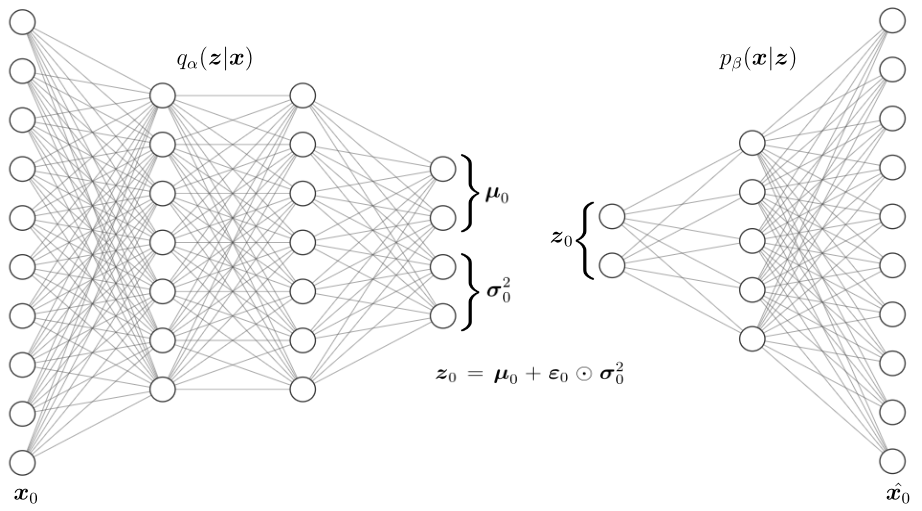
\includegraphics[width=.95\textwidth]{img/vae_visual.png}
  \caption{Visualization of a VAE architecture with $n=10$ and $d=2$.}
  \label{fig:vae_visual}
\end{figure}
The VAE architecture is summarized in Figure \ref{fig:vae_visual}. Note that the VAE does not need to be symmetric; the encoder and decoder can have a different number of hidden layers of different sizes.

\section{Time Series Neural Networks}
In many deep learning applications such as video processing, natural language processing, or dynamical systems, the observed data is time-dependent \cite{kahou2015} \cite{vaswani2017} \cite{gilpin2020}.In such datasets, a single observation of $d$ features can not represented as a vector $\vect x_0 \in \R^d$, but must take into account the $T$ different measurements of the $d$ features, each taken at a different timestep $1 \leq t \leq T$. As such, a data point is represented as a matrix $X_0 \in \R^{d \times T}$, where each column $t$ of $X_0$ gives a snapshot of the observation at time $t$. 

\subsection{Recurrent Neural Networks}
Recurrent Neural Networks (RNN) are the most simple adaptation of neural networks to deal with time-series data. A regular feed-forward neural network layer takes an input vector $\vect x \in \R^d$ and outputs
\begin{equation}
  \vect y = f( W\vect x + \vect b)
  \label{eq:ffn_layer}
\end{equation}
where $W \in \R^{h \times d}$ and $\vect b \in \R^h$ are trainable parameters and $f$ is a non-decreasing activation function \cite{sharma2020}. 

In the time-dependent setting, let $\vect x_t$ be a column of an input $X$. A basic recurrent layer calculates 
\begin{equation}
  \begin{split}
    \vect h_t &= \tanh(W_{hh}\vect h_{t-1} + W_{hx}\vect x_t + \vect b_h) \\
    \vect y_t &= \sigma(W_{hy}[\vect x_t, \vect h_t] + \vect b_y)
\end{split}
  \label{eq:rnn_layer}
\end{equation}
where $W_{hh} \in \R^{h\times h}$, $W_{hx}\in \R^{h\times d}$, $\vect b_h \in \R^h$, $W_{hy} \in \R^{h \times (h+d)}$, and $\vect b_y \in \R^h$ are trainable parameters \cite{elman1990}. The notation $[\vect x_t, \vect h_t]$ refers to vector concatenation. Note that this allows the output $\vect y_t$ to include information from previous time-steps. A visualization of an unfolded RNN is shown in Figure \ref{fig:rnn_visual}.

\begin{figure}[h]
  \centering
  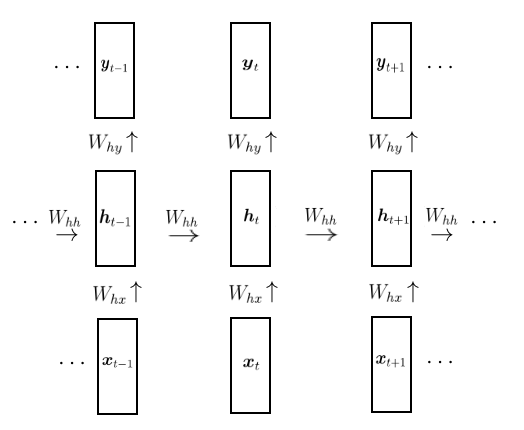
\includegraphics[width=.5\textwidth]{img/rnn_visual.png}
  \caption{Architecture of a recurrent neural network.}
  \label{fig:rnn_visual}
\end{figure}

One issue that RNN face is the exploding or vanishing gradient problem \cite{bengio1994}, where the norm of the gradient can become very large or very small during training. This is due to the fact that partial derivatives calculated during back-propagation between hidden states at time $t_1$ and $t_2$ is found by a product of $t_2 - t_1$ Jacobian matrices \cite{pascanu2013}. As the difference between $t_1$ and $t_2$ increases, the corresponding partial derivatives $\frac{\partial \vect h_{t_1}}{\partial \vect h_{t_2}}$ can exponentially grow or exponentially decay in norm.

Related to the exploding/vanishing gradient issue, RNN experience difficulty in retaining important information for multiple time-steps is difficult. For example, if an important phenomena happens to data point $X_0$ at time $t$, then that information should still influence the values of $\vect h_{t+10}$ and $\vect y_{t+10}$. But the structure described in Equation \ref{eq:rnn_layer} and Figure \ref{fig:rnn_visual} causes the impact of $\vect x_t$ and $\vect h_t$ to fade over time.


\subsection{Long Short-Term Memory Networks}
To combat this issue, Long Short-Term Memory (LSTM) networks were developed by Hochreiter and Schmidhuber \cite{hochreiter1997}. This architecture introduces element-wise multiplication and addition operations in addition to multiple trainable weights matrices which allows for tracking long-term dependencies. An LSTM layer computes a ``cell state'' vector $\vect c_t$, in addition to the hidden layer representation $\vect h_t$. This cell state is updated at each time-step to ``remember'' important information and ``forget'' frivolous information.

The LSTM structure also addresses the exploding/vanishing gradient of RNN. The presence of the cell state $\vect c_t$ ensures that calculating derivatives of long-range dependencies do not include many matrix multiplications \cite{hochreiter1997}.

A single cell of an LSTM can be compared to the middle block in Figure \ref{fig:rnn_visual} containing $\vect h_t$ of an RNN. At time $t$, given an input $t$ $\vect x_t$, previous hidden state $\vect h_{t-1}$, and previous cell state $c_{t-1}$, an LSTM cell uses four trainable weights matrices and four element-wise operations. First compute the ``forget'' vector $\vect f_t$, the ``update'' vector $\vect u_t$, the ``add'' vector $\vect a_t$, and the ``filter'' vector $\vect g_t$.
\begin{equation}
\begin{split}
  \vect f_t &= \sigma(W_f [\vect x_t, \vect h_{t-1}] + \vect b_f) \\
  \vect u_t &= \sigma(W_u [\vect x_t, \vect h_{t-1}] + \vect b_u) \\
  \vect a_t &= \tanh(W_a [\vect x_t, \vect h_{t-1}] + \vect b_a) \\
  \vect g_t &= \sigma(W_g [\vect x_t, \vect h_{t-1}] + \vect b_g)
\end{split}
  \label{eq:lstm_vects}
\end{equation}

The first three vectors in Equation \ref{eq:lstm_vects} are used to perform element-wise operations on $\vect c_{t-1}$ to produce the next cell state $\vect c_t$, and $\vect g_t$ is used in updating $\vect h_t$. Notice that the sigmoid activation function $\sigma(\cdot)$ maps small inputs to near $0$ and large inputs to near $1$, while the hyperbolic tangent activation function $\tanh(\cdot)$ maps small inputs to near $-1$ and large inputs to near $1$. 

Using $\vect f_t$, unimportant aspects (elements near zero) of $\vect c_{t-1}$ are forgotten:
\begin{equation}
  \vect c_{t-1}^* = \vect c_{t-1} \times \vect f_t
  \label{eq:lstm_forget}
\end{equation}
where $\times$ is element-wise multiplication. Next, $\vect u_t$ decides what information to update (elements near one), and $\vect a_t$ gives the value (an increase or decrease) of the information to be updated:
\begin{equation}
  \vect c_t = \vect c_{t-1}^* + \left( \vect u_t \times \vect a_t \right)
  \label{eq:lstm_update}
\end{equation}
where $+$ and $\times$ are element-wise addition and multiplication, respectively. Lastly, compute the next hidden state using $\vect g_t$, which filters the information to be passed to the next network layer and next time-step:
\begin{equation}
  \vect h_t = \tanh(\vect c_t) \times \vect g_t
  \label{eq:lstm_filter}
\end{equation}

\begin{figure}[h]
  \centering
  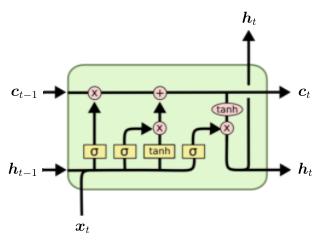
\includegraphics[width=.5\textwidth]{img/lstm_visual}
  \caption{Architecture of a single LSTM cell \cite{olah2015}. Trainable matrix multiplication followed by an activation function are in yellow boxes, and element-wise operations without learned parameters are in red ovals.}
  \label{fig:lstm_visual}
\end{figure}

The architecture of an LSTM is visualized in Figure \ref{fig:lstm_visual}. The forget vector acts as a gate which allows/disallows past information to persist over time, while the update and add vector grabs the data from the current input which is worth updating and remembering.


\subsection{Transformers and Attention}
Though LSTM networks presented a significant breakthrough in natural language processing (NLP), they have been quickly surpassed in the application of language modeling by attention-based methods. These models forgo the recurrent structure of information flow seen in RNN and LSTM for feed-forward layers and similarity scores between time steps. For example, calculating a similarity score between each pair of words in a sentence can help extract deeper context in language models such as transformers \cite{vaswani2017}.

While transformers are large neural networks with many components and parameters, they lean heavily on the attention mechanism. Given a $d$-dimensional feature vector $\vect x_t$ at each time-step $1\leq t\leq T$, define three trainable matrices $W_q$, $W_k$, and $W_v$. These are used to obtain a \textit{query}, \textit{key}, and \textit{value} vectors $\vect q_t$, $\vect k_t$, and $\vect v_t$ for each time-step. Note that these can be arranged into matrices $Q,K,V \in \R^{T\times d}$. Calculated the correlation between observation $t$ and all other time-steps:
\begin{equation}
  \vect c_t = \text{softmax}\left(\frac{K \vect q_t}{\sqrt{d}} \right) \in \R^T
  \label{eq:attn_cor}
\end{equation}


Notice that the matrix multiplication $K \vect q_t$ in Equation \ref{eq:attn_cor} is simply $T$ individual dot-product computations. So the $i$-th entry of $\vect c_t$ gives the similarity between the input at time $t$ and the input at time $i$. The softmax function $\text{softmax}(z_i) = \frac{e^{z_i}}{\sum_{j=1}^T e^{z_j}}$ rescales the dot product calculations so that the sum of the entries of $\vect c_t$ is equal to 1. In applications where an input $\vect x_{t_1}$ is not allowed to see information of future inputs $\vect x_{t_2}$, $t_1<t_2$, the corresponding entries of $K\vect q_{t_1}$ are masked to be $-\infty$. This causes the entries $c_{ti} = 0$ when $i > t$.

Next, the attention is calculated as 
\begin{equation}
  \vect a_t = V \vect c_t \in \R^d
  \label{eq:attn}
\end{equation}
The attention vector $\vect a_t$ is a weighted sum of the value vectors of each other time-step, weighted by the correlation scores in Equation \ref{eq:attn_cor}. The attention calculation can also be written more generally:
\begin{equation}
  A = \text{softmax}\left(\frac{QK^\top}{\sqrt{d}} \right) V \in \R^{T \times d}
  \label{eq:attn_matrix}
\end{equation}

In attention networks, the attention vectors $\vect a_t$ are individually sent through feed-forward layers. For example, transformers calculate attention and then use three feed-forward layers in a single ``block'' \cite{vaswani2017}. These blocks are stacked on top of each other up to six times to obtain deeper and deeper contextualization of the input sequence \cite{dai2019}. Eventually, this contextualization is plugged into a final prediction layer, depending on the application.

It should be pointed out that transformers and attention networks were developed for the NLP application. So in this case, a sequence of $T$ inputs represents a sentence of length $\leq T$ and an input vector $\vect x_t$ is a $d$-dimensional learned representation of an individual word \cite{mikolov2013}. Then the correlation score in Equation \ref{eq:attn_cor} is quantifying the relationship between pairs of words in the sentence.


 % split up this section and moved content
\chapter{The ML2P-VAE Method for IRT Parameter Estimation}\label{ch:ml2pvae_methods}
The primary contribution of this thesis is the development of a method for IRT parameter estimation which uses a modified VAE. The method, titled ``ML2P-VAE'', is interesting from multiple perspectives. In the application area, it is an unconventional approach that produces estimates with similar accuracy of traditional parameter estimation techniques. Further, ML2P-VAE scales much better than traditional methods as the number of latent abilities becomes large. 

In traditional IRT parameter estimation, large datasets present a \textit{burden} -- they require more parameters to be estimated and a larger number of computations. But ML2P-VAE, through the lens of machine learning, views large datasets as a \textit{blessing} -- bigger data provides more information (more responses $u_{ij}$) to learn from in order to more accurately reconstruct inputs. A better reconstruction of input responses directly correlates with improved parameter estimates.

In the field of machine learning, ML2P-VAE is seen as an unsupervised learning technique which yields explainable results. A variational autoencoder is used in an unorthodox way -- VAE are typically used as generative models where only the decoder is used at test-time. In ML2P-VAE, test-time involves feeding student responses through the encoder to obtain a prediction of latent traits -- a result of an interpretable hidden neural network layer. The trainable parameters in the decoder are able to be understood in a real-world context -- they serve as estimates to item parameters to the ML2P model from Section \ref{sec:mirt}. In fact, the entire VAE decoder can be interpreted as an approximate ML2P model (see Equation \ref{eq:ml2p}).

Another important contribution of this thesis is the development of a novel neural network architecture which fits a VAE to a multivariate Gaussian distribution $\mathcal{N}(\vect \mu, \Sigma)$ where the latent code is correlated. This is a significant difference from previous implementations of VAE, which always assume that the dimensions of the latent code are independent of each other (see Equation \ref{eq:ind_gauss_kl}). The more general architecture presented in this thesis is particularly helpful when additional domain knowledge of the latent code is accessible.

\section{ML2P-VAE Method Description}\label{sec:ml2p_vae}
Given an assessment with $n$ items which tests $K$ latent skills, assume that $N$ students take this exam. Data is given as an $N \times n$ binary matrix $U$, as in Equation \ref{eq:responses}. No information about the student latent ability parameters $\vect \Theta \in \R^K$ or the item parameters $a_{ik}$ and $b_i$ is provided. However, assume that there is access to an expert-annotated binary $Q$-matrix detailing the item-skill associations, described by Equation \ref{eq:q_matrix}. Implicitly, we assume that the student responses were generated by the ML2P model, introduced in Equations \ref{eq:ml2p} and \ref{eq:ml2pq}:
\begin{equation}
  P(u_{ij} = 1 | \vect \Theta_j; \vect{a_i}, b_i) = \frac{1}{1 + \exp\left(-\sum_{k=1}^K q_{ik} a_{ik} \theta_{jk} + b_i \right)}
  \label{eq:ml2p_again}
\end{equation}

This assumption directly links IRT with VAE. Recall from Section \ref{sec:vae_derive} that the VAE decoder parameterizes the posterior distribution $p_\beta(\vect x | \vect z)$, seen in Figure \ref{fig:vae_visual}. Replace the observed data $\vect x$ with the student responses $\vect u_j$ and the latent code $\vect z$ with the latent traits $\vect \Theta_j$, and we see that Equation \ref{eq:ml2p_again} provides an explicit form for the posterior distribution $p_\beta(\vect x | \vect z)$ learned by a VAE decoder. Recall that the subscript $\beta$ references a particular setting of the weights in the VAE decoder, drawing parallel with the item parameters $\vect a_i$ and $b_i$. Though $\vect a_i$ and $b_i$ are unknown, the constraints imposed by entries in the $Q$-matrix $q_{ik}$ provide enough structure for the neural network to learn these values during the training process, so long as $Q$ is sufficiently sparse \cite{jiang2018}.

A number of specifications are required in order to use a VAE as an IRT parameter estimation method. First, set up the neural network so that the input and output layers each have $n$ nodes, each node representing one item. The inputs are the binary response vectors $\vect u_j$ defined in Equation \ref{eq:responses} and the outputs are approximations of the probability of student $j$ answering each item correctly. 

The dimension of the hidden distribution (the output of the encoder) must be equal to $K$, the number of latent skills. The usual VAE loss function described in Equation \ref{eq:vae_loss} is still used to optimize ML2P-VAE. The KL-Divergence term acts as a regularizer between the posterior distribution produced by the encoder $q_\alpha(\vect \Theta_j | \vect u_j)$ and prior distribution of latent abilities $p(\vect \Theta)$. Usually, these distributions are assumed to be independent Gaussian, but we extend this idea to a more general multivariate Gaussian distribution where the latent traits $\vect \Theta$ are correlated in Section \ref{sec:cov}.

The modifications to a typical VAE architecture are focused on the decoder. No hidden layers are used in the decoder. Instead, a non-dense matrix of weights connects the decoder input to the decoder output. The non-zero weights here are determined by the binary $Q$-matrix from Equation \ref{eq:q_matrix}; recall that the input to the decoder has $K$ nodes, the decoder output has $n$ nodes, and $Q \in \{0,1\}^{n \times K}$. So for a trainable weight $w_{ik}$ in the VAE decoder, if $q_{ik}=0$, then fix $w_{ik}=0$ as well, and it will never be updated during the training process. This modification is key to allowing interpretation of the hidden latent distribution of a VAE, and is visualized in Figure \ref{fig:ml2pvae_visual}.

The ML2P-VAE method requires the use of the sigmoid activation function
\begin{equation}
  \sigma(z_i) = \frac{1}{1 + e^{-z_i}} = \frac{1}{1 + \exp\left(- \sum_{k=1}^K w_{ik} \alpha_k + \beta_i \right)}
  \label{eq:sigmoid}
\end{equation}
in the output layer (see Appendix \ref{apdx:activation_fcns}). Here, $z_i = \sum_{k=1}^K w_{ik}\alpha_{k} + \beta_i$ is the input to the $i$-th node in the decoder, where $w_{ik}$ is the weight between the $k$-th and $i$-th nodes in the decoder input and decoder output layer and $\beta_i$ is the additive bias in the output layer. $\alpha_k$ is the activation of the $k$-th node in the decoder input layer, which is the sample drawn from the posterior distribution produced by the encoder. 

Note the similarity between Equation \ref{eq:sigmoid} and the ML2P model in Equation \ref{eq:ml2p_again}. The constraint on the weights along with the sigmoid activation function allows for interpretation of the VAE decoder as an approximate ML2P model.

Specifically, the nonzero decoder weights $w_{ik}$ can be interpreted as estimates to the discrimination parameters $a_{ik}$, the output bias $\beta_i$ can be interpreted as estimates to the difficulty parameters $b_i$, and the activations $\alpha_k$ produced by the encoder (given the response input $\vect u_j$) can be interpreted as estimates to the student ability parameter $\theta_{kj}$. All of this explainability is allowed by the constraint on the decoder weights matrix imposed by the binary $Q$-matrix.

Further modifications can improve the performance of ML2P-VAE. In IRT, discrimination parameters are assumed to be non-negative, because an increase in a skill should never decrease the probability of answering an item correctly. With this assumption in mind, requiring all decoder weights $w_{ik} \geq 0$ avoids a potential identification problem, since $\theta^* \cdot a^* = (-\theta^*)\cdot(-a^*)$.

To summarize, the ML2P-VAE model takes as input the student responses $\vect u_j$ and maps them through a VAE encoder to estimates of the student's latent abilities $\vect \Theta_j$. This estimate is sent through a \textit{modified} VAE decoder, whose trainable parameters serve as estimates to the ML2P model. The final output of the VAE decoder is the estimated probability of student $j$ answering each item $i$ correctly, $P_{ij} = \sigma(\vect a_i^\top \vect \Theta_j + b_i)$ as described in Equation \ref{eq:sigmoid}, which is treated as a reconstruction of the inputs $u_{ij}$.


\subsection{Full Covariance Matrix Implementation}\label{sec:cov}
In this section, we detail a novel architecture for a VAE which fits observed data to a latent space with correlated latent code, $\mathcal{N}(\vect \mu, \Sigma)$. There are many publicly available code examples of VAE implementations which assume the latent space follows a standard normal distribution $\mathcal{N}(0,I)$. But it is not so common to train a VAE which assumes that the latent prior $p(\vect \Theta)$ has correlated dimensions. Since most applications do not attempt to interpret hidden layers of a VAE, there is no available information on the correlations of abstract, unobservable features. Additionally, it can be beneficial to force the latent dimensions to be independent of one another when considering the usual applications of VAE.

In IRT, we may be able to quantify the correlation between latent abilities, presenting need for the ML2P-VAE model to take advantage of this information. This task is nontrivial due to two mechanisms of the VAE:
\begin{itemize}
  \item[(1)] sampling from the learned distribution as in Equation \ref{eq:bernoulli}, and
  \item[(2)] calculating Kullback-Leibler Divergence as in Equation \ref{eq:ind_gauss_kl}.
\end{itemize}
These two characteristics must be addressed when constructing a neural architecture which accounts for correlated $\vect \Theta$.

After training a VAE, sending a data point $\vect u_0$ through the encoder needs to give a set of values that correspond to a probability distribution. For a $K$-dimensional multivariate Gaussian distribution, these values are a vector $\vect \mu_0 \in \R^K$ and a symmetric, positive-definite matrix $\Sigma_0 \in \R^{K\times K}$. Sampling from $\mathcal{N}(\vect \mu_0, \Sigma_0)$ requires a matrix $G_0$ such that $G_0 G_0^\top = \Sigma_0$. This matrix factorization $G_0$ is not necessarily unique, but it can be convenient to use the Cholesky decomposition of $\Sigma_0$ where $G_0$ is lower triangular \cite{atkinson}. The sample from the multivariate Gaussian distribution is calculated as
\begin{equation}
  \vect z_0 = \vect \mu_0 + G_0 \vect{\e_0}
  \label{eq:multivariate_sample}
\end{equation}
where $\vect{\e_0} = (\e_1, \ldots, \e_K)^\top $and $\e_i \sim \mathcal{N}(0,1)$. 

The KL-Divergence between two $K$-variate Gaussian distributions is given as
\begin{equation}
\begin{split}
  &\mathcal{D}_{KL}\left[\mathcal{N}(\vect \mu_0, \Sigma_0) || \mathcal{N}(\vect \mu_1, \Sigma_1) \right] = \\
&\frac{1}{2} \left( \tr(\Sigma_1^{-1}) \Sigma_0) + (\vect \mu_1 - \vect \mu_0) \Sigma_1^{-1} (\vect \mu_1 - \vect \mu_0) - K + \ln\left( \frac{\det \Sigma_1}{\det \Sigma_0 }\right) \right)
  \label{eq:kl_multivariate}
\end{split}
\end{equation}
When using this in a VAE, $\mathcal{N}(\vect \mu_1, \Sigma_1)$ corresponds to the prior $p(\vect \Theta)$, and so $\vect \mu_1$ and $\Sigma_1$ are constant. $\Sigma_1^{-1}$ only needs to be computed once, and this matrix inversion won't cause computation time problems at any point. Note that Equation \ref{eq:kl_multivariate} requires computing $\ln \det \Sigma_0$, so we must have $\det \Sigma_0 > 0$ at all times during training. Recall that $\vect \mu_0$ and $\Sigma_0$ correspond to the input $\vect u_0$, and also depend on all the trainable weights and biases in the VAE encoder. These parameters are usually initialized randomly, and the user has little control over their values during training. If $\det \Sigma_0 \leq 0$ for any input $\vect u_0$ at any point while training, then it is not possible to compute the loss and gradient to perform backpropagation updates. Thus, a specific architecture which guarantees that $\det \Sigma_0 > 0$, regardless of the input $\vect u_0$ or encoder parameters, is required.

This architecture is described as follows. The input and output to the neural network consists of $n$ nodes, each representing an item on an assessment which assesses $K$ skills. Given an input $\vect u_0$ and after a sufficient number of hidden layers of sufficient size, the encoder outputs $K + \frac{K(K+1)}{2}$ nodes. The first $K$ nodes represent the mean vector $\vect \mu_0$, and the remaining $\frac{K(K+1)}{2}$ nodes are arranged into a lower triangular matrix $L_0 \in \R^{K\times K}$. The covariance matrix is obtained using the matrix exponential $\Sigma_0 = e^{L_0} \cdot \left( e^{L_0} \right)^\top$.

\begin{theorem}
  Let $L_0$ be a lower triangular matrix, and define $\Sigma_0 = e^{L_0} \cdot \left(e^{L_0}\right)^\top$. Then $\Sigma_0$ is symmetric, positive-definite, and has positive determinant.
  \label{thm:cov_vae}
\end{theorem}
\begin{proof}
  Consider any lower triangular $L_0 \in \R^{K\times K}$. Define 
  \[G_0 = e^{L_0} = \sum_{n=1}^\infty \frac{L_0^n}{n!} = I + L_0 + \frac{1}{2} L_0 \cdot L_0 + \cdots\]
  $G_0$ is lower triangular, since addition and multiplication of matrices preserve this property. Further, $G_0$ is nonsingular, because $\det G_0 = \det(e^{L_0}) = e^{\tr L_0} > 0$.

  Set $\Sigma_0 = G_0 G_0^\top$. Clearly, $\Sigma_0$ is symmetric as $\Sigma_0^\top = (G_0 G_0^\top)^\top = G_0 G_0^\top = \Sigma_0$. Further, 
  \[\det \Sigma_0 = \det \left(G_0 G_0^\top \right) = \det G_0 \cdot \det G_0^\top = e^{\tr L_0} \cdot e^{\tr L_0} > 0.\]
So now for any nonzero $\vect x \in \R^K$,
  \[\langle \Sigma_0 \vect x, \vect x \rangle = \vect x^\top \Sigma_0 \vect x = \vect x^\top G_0 G_0^\top \vect x = \langle G_0^\top \vect x, G_0^\top \vect x \rangle = ||G_0 \vect x||_2^2 > 0\]
  Therefore, $\Sigma_0$ is positive-definite.
\end{proof}

Theorem \ref{thm:cov_vae} shows that in this specific neural network architecture, $\Sigma_0$ can be interpreted as a covariance matrix. Thus, the VAE encoder maps a data point $\vect u_0$ to a multivariate Gaussian distribution $\mathcal{N}(\vect \mu_0, \Sigma_0)$. Additionally, the sampling operation in Equation \ref{eq:multivariate_sample} and KL-Divergence calculation in Equation \ref{eq:kl_multivariate} can always be carried out without issue.

\begin{figure}[h]
  \centering
  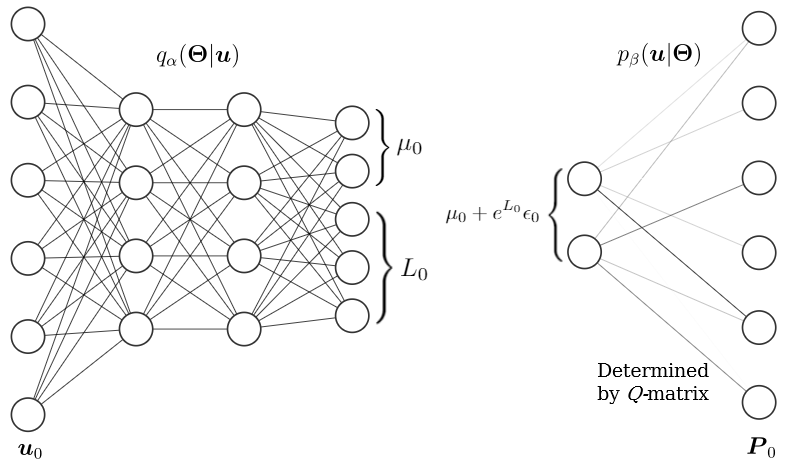
\includegraphics[width=.85\textwidth]{img/ml2pvae_visual.png}
  \caption{Visualization of the ML2P-VAE architecture for two correlated latent traits and six input items. Note that the trainable weights matrix in the decoder is not dense, but is determined by the given $Q$-matrix.}
  \label{fig:ml2pvae_visual}
\end{figure}

A visualization of the ML2P-VAE architecture for correlated latent traits is shown in Figure \ref{fig:ml2pvae_visual}. At test time, the estimate of the latent skills of a student with responses $\vect u_0$ is obtained via $\vect \Theta_0 = \vect \mu_0$. The output reconstruction $\vect P_0$ refers  to the reconstruction of the input $\vect u_0$, also interpreted as the probability of student $0$ answering each question correctly:
\[P_{i0} = P(u_{i0} = 1 | \vect \Theta_0; \vect a_i, b_i)\]



\subsection{Variants of ML2P-VAE}\label{sec:variants}

We consider three scenarios for using ML2P-VAE in practice: (a) the best case scenario where the covariance matrix between all latent traits is fully known, (b) the exact covariance matrix unknown, so it is estimated using other methods, and (c) we simply assume that all traits are independent. These three situations result in three variations of the ML2P-VAE method: ML2P-VAE$_{full}$, ML2P-VAE$_{est}$, and ML2P-VAE$_{ind}$, respectively. 

In order to estimate the correlations between latent traits for use of ML2P-VAE$_{est}$ in scenario (b), the student response matrix $U \in \R^{N\times n}$ is multiplied by the $Q$-matrix $Q \in \R^{n \times K}$. Denote $M = UQ \in \R^{N\times K}$. Then the Pearson correlation of the columns of $M$ produce an approximate correlation matrix $\hat \Sigma \in \R^{K \times K}$, where each entry $\hat \sigma_{kl}$ gives the approximate correlation between latent traits $k$ and $l$.
\begin{equation}
  \hat \sigma_{kl} = \frac{\sum_{i=1}^N (k_i - \bar k)(l_i - \bar l)}{\sqrt{\sum_{i=1}^N(k_i - \bar k)^2} \sqrt{\sum_{i=1}^N (l_i - \bar l)^2}}
  \label{eq:approx_cor_mat}
\end{equation}
where $\bar k$ and $\bar l$ are the mean values of the $k$-th and $l$-th columns of $M$, respectively.

A final variation of ML2P-VAE comes when the IRT model to be estimated is changed. If assuming that student responses are generated according to the Rasch model in Equation \ref{eq:rasch} rather than the ML2P model from Equation \ref{eq:ml2p}, then another variation of VAE parameter estimation methods can be considered. A more appropriate name for this alternative estimation method is Rasch-VAE.

Since there are no discrimination parameters in the Rasch model, only item difficulties and student abilities need to be estimated. To account for this, the weights in the VAE decoder are restricted to be \textit{equal} to the $Q$-matrix, i.e. $w_{ik} = q_{ik}$. This still allows for interpretation of the learned distribution of the VAE as estimates to student abilities $\vect \Theta$, while requiring ``discrimination parameters'' to be equal to either one or zero, fitting more closely to Equation \ref{eq:rasch}.

%
\section{\textbf{ML2Pvae} Software Package for R}
The ML2P-VAE method for parameter estimation has been compiled in an easy-to-use software package for R \cite{r_package}. This allows researchers who may not have experience with neural networks to implement ML2P-VAE methods on a data set of their choosing. The package \textbf{ML2Pvae} is available on the Comprehensive R Archive Network (CRAN) and can be easily installed using the R command:
\begin{lstlisting}[language=R, numbers=none]
install.packages('ML2Pvae')
\end{lstlisting}

\subsection{Package Functionality}
\textbf{ML2Pvae} uses Tensorflow and Keras to build and train neural networks, but no knowledge of these libraries are required in order to use \textbf{ML2Pvae}. The package exports five functions available to the user. Two of these are used to construct Keras models, with optional parameters specifying the architecture of the neural network. The only parameters which require input from the user are the number of items on the exam, the number of latent abilities that the exam assesses, and the $Q$-matrix relating items and abilities.

The optional inputs in the model construction include a covariance matrix for latent traits, allowing for correlated skills and the implementation described in Section \ref{sec:cov}. An important feature for model selection gives the choice of the number of item parameters to use in the logistic IRT model. Though the package is called \textbf{ML2Pvae} for the Multidimensional Logistic 2-Parameter model, the package allows for estimating parameters with the Rasch model, so that Rasch-VAE from Section \ref{sec:variants} can be implemented. In this case, there is only a difficulty parameter for each item; each  discrimination parameter is fixed to be equal to 1. Other options when building ML2P-VAE models specify the number, size and activation functions of the hidden layers in the encoder.

Using the Keras models returned by the construction functions, \textbf{ML2Pvae} provides a function that can be used to train the VAE on data. This function acts as a wrapper for the \verb!fit()! method in the Keras package. The final two methods obtain item parameter estimates and student ability parameter estimates. This is done by grabbing the correct weights/biases from the decoder and feeding student responses through the encoder, respectively. A more detailed description of the functionality of \textbf{ML2Pvae}, along with a code tutorial, is given in Appendix \ref{apdx:software}.


\chapter{ML2P-VAE Results and Discussion}\label{ch:ml2pvae_results}

The ML2P-VAE method has been used in a various settings in multiple publications related to educational measurement \cite{aied_paper, ml_paper, ijcnn_paper}. The first paper, ``Interpretable Variational Autoencoders for Cognitive Models'' (\textit{International Joint Conference on Neural Networks} 2019), introduced the ML2P-VAE method and gives some preliminary results on a small simulated data set. The second, ``Autoencoders for Educational Assessment'' (\textit{Conference on Artificial Intelligence in Education} 2019), displays the advantages that a VAE holds over a regular autoencoder in the task of parameter estimation. The final publication, ``Estimation of Multidimensional Item Response Theory Models with Correlated Latent Variables using Variational Autoencoders'' (\textit{Machine Learning} 2021), compares different variations of ML2P-VAE with traditional parameter estimation methods on both real and simulated data sets of various sizes, along with introducing the novel VAE architecture described in Section \ref{sec:cov}.

In this chapter, we first summarize all datasets used in experiments, then present all results from each publication. Finally, we explore future extensions of the ML2P-VAE method and summarize the contributions of this research.

\section{Description of Data Sets}\label{sec:irt_data}
\subsubsection*{Sim-ECPE} This simulated data set is designed to mirror the real-world Examination for the Certificate of Proficiency in English, detailed further in the next dataset description. Sim-ECPE has 28 items assessing 3 latent traits. Values for the item parameters in the ML2P model were generated from a uniform distribution so that $a_{ik} \in [0.25, 1.75]$ and $b_i \in [-3,3]$. The range for the discrimination parameters was chosen such that $0.25 \leq MDISC_i \leq 1.75$ for all $i$ (see Equation \ref{eq:mdisc}). Up to 10,000 student abilities $\vect \Theta \in \R^3$ were sampled from $\mathcal{N}(0,I)$, and experiments are performed using different numbers of students $N$. Note that in Sim-ECPE, it is assumed that the latent traits are independent. We use a $Q$-matrix consistent with previous literature \cite{daSilva2018, templin2013, henson2007}.

\subsubsection*{ECPE} The Examination for the Certificate of Proficiency in English (ECPE) is an exam with 28 items designed to certify learners of the English language. The set of responses we use is available in the \textbf{CDM} package for R \cite{cdm}. This includes 2,922 students and a $Q$-matrix for three skills - ``morphosyntactic rules'', ``cohesive rules'', and ``lexical rules''. Since this is a real-world data set, there are not ``true'' values of item or student ability parameters to compare with the model estimates, so we must compare our results with previous literature.

\subsubsection*{Sim-6} A moderately-sized simulated data set, Sim-6 has 50 items evaluating 6 latent traits. The $Q$-matrix is also generated randomly, where each entry $q_{ik}$ is sampled from $\text{Bern}(0.2)$. To ensure each item requires at least one latent ability, if a row $q_{i:} = 0$ after sampling, then one random element in the row is changed to a 1. The discrimination parameters are chosen so that $a_{ik} \in [0.1, 1.3]$ and $b_i \in[-3,3]$ and that $0.25 \leq MDISC_i \leq 1.75$. Abilities $\vect \Theta \in \R^6$ of 20,000 students were sampled from $\mathcal{N}(0, \Sigma)$, where $\Sigma$ is a correlation matrix with all positive values generated using the SciPy package \cite{SciPy}.

\subsubsection*{Sim-20} This large data set is generated in a similar manner to Sim-6, but includes 50,000 students, 200 items, and 20 latent traits. The $Q$-matrix was generated in the same way as that of Sim-6, where $q_{ik} \sim \text{Bern}(0.2)$. The difficulty parameters were sampled uniformly so that $b_i \in [-3,3]$, and the discrimination parameters were sampled uniformly so that $a_{ik} \in [0.1, 0.9]$. As in Sim-6, the 20 latent abilities are correlated with one another (i.e. $\vect \Theta \sim \mathcal{N}(0, \Sigma)$), and the correlation matrix is generated in the same manner as in Sim-6.
\subsubsection*{Sim-4} Sim-4 contains 3,000 student responses to an exam with 27 items over 4 latent abilities. Another simulated dataset, the covariance matrix and $Q$-matrix were chosen more deliberately than the previous two datasets. Of the 4 skills in the correlation matrix, one of them is entirely independent of the other three. The other three latent abilities had correlations of 0.25, 0.1, and 0.15 between them. These correlation values are much smaller than those of Sim-6 or Sim-20, resulting in a covariance matrix that is closer to the identity. The $Q$-matrix was chosen so that it contained 16 simple items (items requiring only one skill), 6 items requiring 2 latent abilities, 4 items requiring 3 latent abilities, and one item requiring all 4 skills. In this way, each of the possible $\binom{4}{k}$ combinations is present in the $Q$-matrix, for $k\in \{1,2,3,4\}$.

\section{Quantitative Results}

\subsection{Preliminary Results}\label{sec:prelim}
This section describes the results presented at IJCNN 2019 \cite{ijcnn_paper}, when the ML2P-VAE model was initially proposed. All experiments were performed on the Sim-ECPE dataset.

The latent traits values were generated independently from a $\mathcal{N}(0,I)$ distribution to compose three datasets with different sample sizes ($N$): $500$, $5,000$, and $10,000$ subjects. All figures included in this section were generated using the largest set $N=10,000$. The smaller sample size was fixed with the goal of comparison to previous results presented in the literature for the ML2P model, which use the traditional estimation process MCMC. The current results can be directly compared to the ones published by da Silva et al. \cite{daSilva2018}, since the simulation scenarios are the same. The other two sample sizes were chosen to study the improvement of the estimation accuracy for the proposed model when provided larger sets of data.

Given a subject's latent traits $\vect \Theta_j$, we generate ten different replicates of responses using the ML2P-Q method \cite{daSilva2018} described in Equation \ref{eq:ml2pq}. After we have ten sets of responses for $N$ subjects, we train ten separate instances of our model and use the learned parameters from these networks to estimate $\hat{\vect a}$, $\hat{\vect b}$, and $\hat{\vect \Theta}$.

The architecture of the variational autoencoder, implemented using TensorFlow, is as follows: The encoder has an input layer of 28 nodes (one for each item), a hidden layer with 10 nodes, and outputs the distribution of the 3 latent traits, requiring 6 nodes. As mentioned in Section \ref{sec:ml2p_vae}, the decoder has no hidden layers, and simply maps the 3 latent traits to the 28 items. The nonzero weights of the decoder are determined by the $Q$-matrix. Further, these weights are restricted to be non-negative and we use a sigmoidal activation function, which lines up with how the data was simulated with ML2P-Q. 

Because of this similarity, we are able to interpret the weights and biases in the decoder of the VAE as estimates of the IRT parameters in Equation \ref{eq:ml2p_again} used to generate the data. Though the encoder is still a black box, the VAE is constructed in a way so that we can interpret the weights and biases in the decoder.

\begin{figure}[h]
  \centering
\minipage{0.5\textwidth}
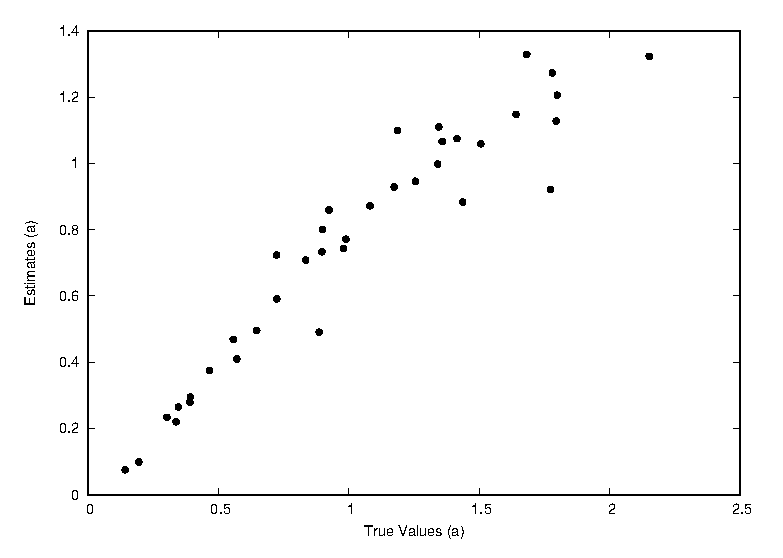
\includegraphics[width=\textwidth]{img/ijcnn_results/10k_a.eps}
   \endminipage\hfill
 \minipage{0.5\textwidth}
 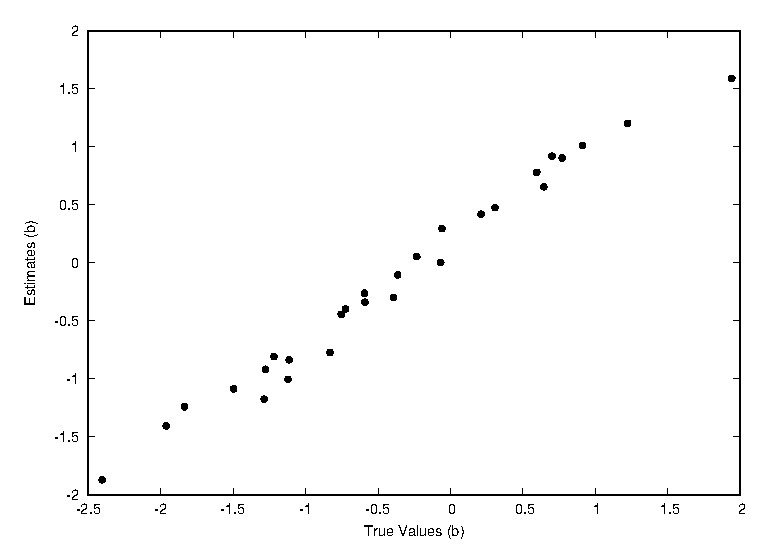
\includegraphics[width=\textwidth]{img/ijcnn_results/10k_b.eps}
   \endminipage\hfill
   \caption{True versus estimated values for discrimination parameters (left) and difficulty parameters (right) with sample size 10,000.}
  \label{fig:a_b_10k}
\end{figure}

In the left plot of Figure \ref{fig:a_b_10k}, we can see a clear correlation between the discrimination parameters used to generate the dataset and the weights in the decoder. There is an even stronger correlation between the difficulty parameters and the biases in the output layer, as seen in the right plot of Figure \ref{fig:a_b_10k}.

Estimates of the discrimination and difficulty parameters yield an improved interpretation of the neural network. The estimates for $a_{ik}$ can be used to quantify the ability of an item to discriminate between individuals with different levels of knowledge. Smaller values correspond to an item with little discriminatory power and larger values correspond to an item that can easily discriminate between individuals with different levels of knowledge. Similarly, the estimates of $b_i$ allow quantification of the difficulty of an item, again with smaller values corresponding to an easier item and larger values corresponding to a more difficult item.

We use root mean square error (RMSE), correlation (CORR), and absolute value of the relative bias (AVRB) between the estimated and true values of the parameters to evaluate the accuracy of parameter estimates. The absolute value of the relative bias (AVRB) was defined as: 
\begin{equation}
\text{AVRB}_i = \left| \frac{\left(\frac{1}{10} \sum_{r=1}^{10} \hat \lambda_{ir}\right) - \lambda_{i}}{\lambda_i} \right|,
\label{eq:replicates}
\end{equation}
where $\lambda_i$ refers to one of the true parameters of the model ($a_{ik}$, $b_i$, or $\theta_{jk}$) and $\hat \lambda_{ir}$ refers to the respective estimate for data replicate $r$. These are shown in Table \ref{tab:ijcnn_param}. As we increase the sample size of the dataset, we see an increase in correlation for all parameters. The error measures of the estimates to $a_{ik}$ decrease, as is expected. Oddly, the error measures for $b_i$ increase as the number of students increases - this issue is left for future work. However, this does not seem to affect the correlation between true and estimated $b_i$.

In general, it can be noted that while there is high correlation between true and estimated item parameters, the RMSE values are not particularly low. This is likely because the scale of the estimates is off -- though the true values $b_i \in [-3,3]$, the estimates obtained were significantly smaller, $\hat b_i \in [-1,1]$, with one exception. So the difference between true and estimated values is sizable, even though they exhibit a strong linear relationship.

\begin{table}[h]
\begin{center}
  \begin{tabular}{ccccc}
    \hline
    &&AVRB&&\\
    \hline
    Size  & $\vect a_{:1}$ & $\vect a_{:2}$ & $\vect a_{:3}$ & $\vect b$ \\
    \hline
    500   & 0.779 & 0.699 & 0.759 & 1.188 \\
    5,000 & 0.539 & 0.281 & 0.585 & 1.673 \\
    10,000  &0.284  & 0.159 & 0.264 & 1.894 \\
    \hline
  \end{tabular}
\end{center}

\begin{center}
  \begin{tabular}{ccccc}
    \hline
    &&RMSE&&\\
    \hline
    Size  & $\vect a_{:1}$ & $\vect a_{:2}$ & $\vect a_{:3}$ & $\vect b$ \\
    \hline
    500   & 0.976 & 0.931 & 0.850 & 1.038 \\
    5,000 & 0.587 & 0.823 & 0.414 & 1.494 \\
    10,000  & 0.322 & 0.346 & 0.264 & 1.670 \\
    \hline
  \end{tabular}
\end{center}

\begin{center}
  \begin{tabular}{ccccc}
    \hline
    &&CORR&&\\
    \hline
    Size  & $\vect a_{:1}$ & $\vect a_{:2}$ & $\vect a_{:3}$ & $\vect b$ \\
    \hline
    500   & 0.457 & 0.547 & 0.381 & 0.987 \\
    5000  & 0.779 & 0.710 & 0.990 & 0.982 \\
    10000   & 0.924 & 0.920 & 0.986 & 0.990 \\
    \hline
  \end{tabular}
\end{center}
\caption{Error measures for item parameter estimates.}
\label{tab:ijcnn_param}
\end{table}

The encoder of our VAE also holds predictive power. Given a subject's assessment results, we feed this information forward through the encoder and return a prediction of that subject's latent traits. In Figures \ref{fig:10kt1}, \ref{fig:10kt2}, and \ref{fig:10kt3}, we observe an explicit relationship between the learned distributions $\hat{\theta}_k$ of the VAE and the latent traits $\theta_k$ for $k\in\{1,2,3\}$. The plots seem to have a sigmoidal tendency, rather than linear. This is not ideal, as it causes our model to struggle with accurately predicting the latent traits of subjects who have either very high or very low latent trait values. 
\begin{figure}[h!]
\minipage{0.45\textwidth}
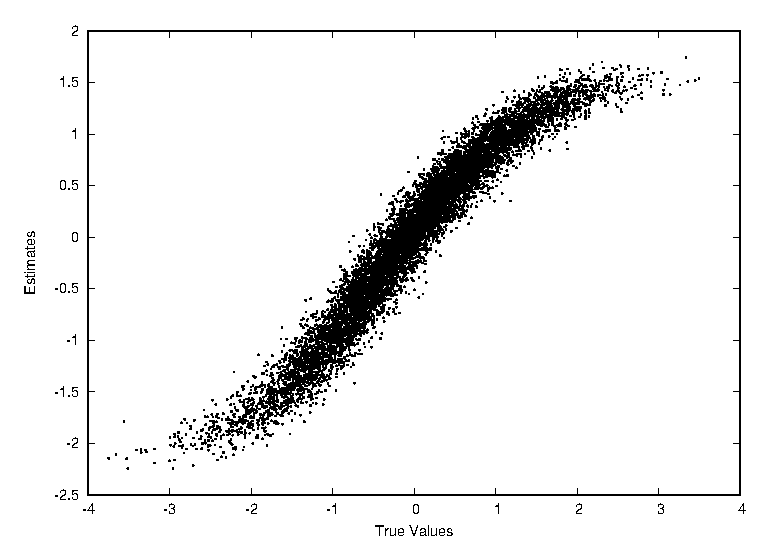
\includegraphics[width=\textwidth]{img/ijcnn_results/10k_t1_scaled.eps}
\caption{$\hat{\theta}_1$ estimates for the first latent variable.}
\label{fig:10kt1}
\endminipage\hfill
\minipage{0.45\textwidth}
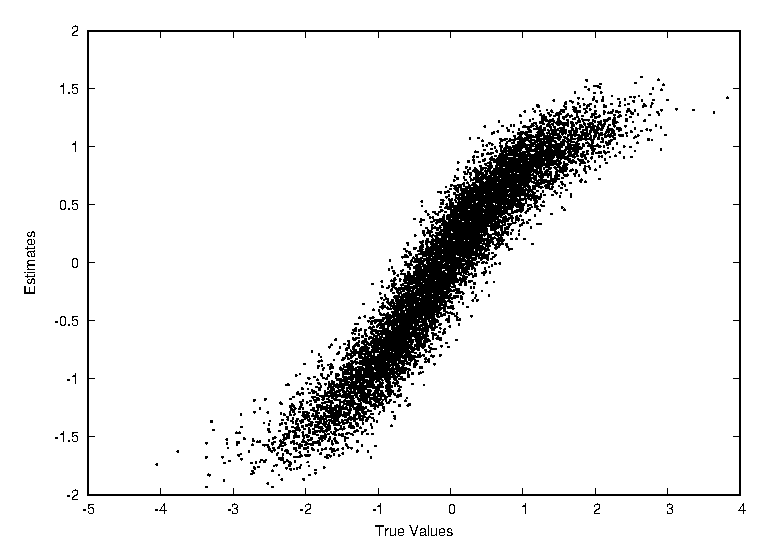
\includegraphics[width=\textwidth]{img/ijcnn_results/10k_t2_scaled.eps}
\caption{$\hat{\theta}_2$ estimates for the second latent variable.}
\label{fig:10kt2}
\endminipage\hfill
\linebreak
\minipage{0.45\textwidth}
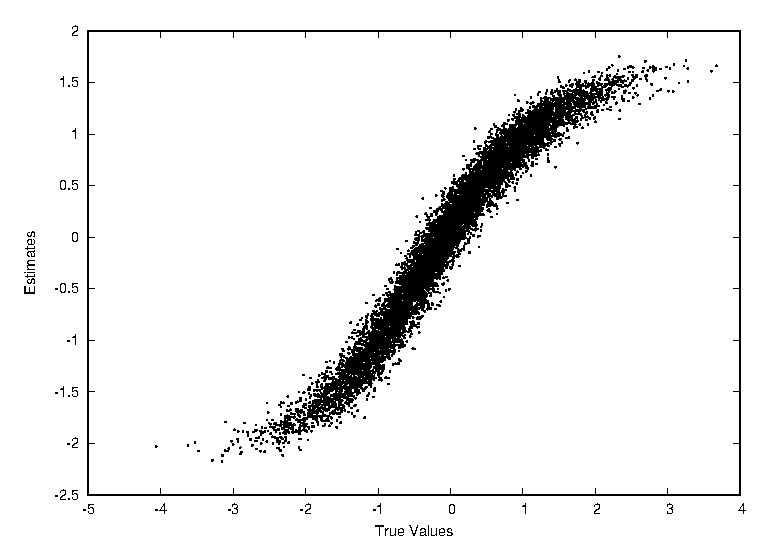
\includegraphics[width=\textwidth]{img/ijcnn_results/10k_t3_scaled.eps}
\caption{$\hat{\theta}_3$ estimates for the third latent variable.}
\label{fig:10kt3}
\endminipage\hfill
\minipage{.45\textwidth}
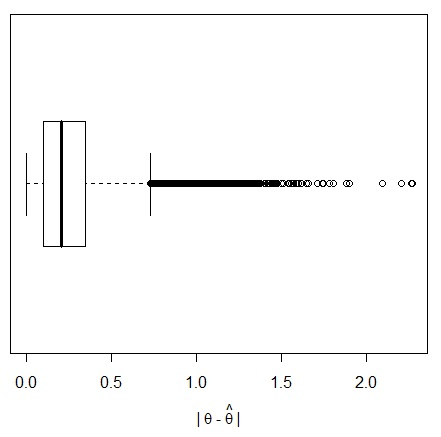
\includegraphics[height=0.7\textwidth,width=\columnwidth]{img/ijcnn_results/BxpTheta.jpg}
\caption{Absolute differences between true values and estimates of $\vect \Theta$.}
\label{fig:boxt10k}
\endminipage\hfill
\end{figure}


The accuracy of these estimates is shown in Figure \ref{fig:boxt10k}. Nearly 90\% of the individuals have the absolute values of the difference between estimates and true values under 0.5, which improves upon the results of the traditional estimation methods in MIRT \cite{daSilva2018}, which achieved approximately 75\% of the individuals with absolute bias under 0.5. The outliers (points outside the box) in Figure \ref{fig:boxt10k} are the left and right parts of the sigmoid shapes seen in Figures \ref{fig:10kt1}, \ref{fig:10kt2}, and \ref{fig:10kt3}.

\subsubsection{Remarks}
One drawback of the proposed model is that it requires a much larger sample size to obtain comparable results. However, despite the larger sample size, the running time of our neural network method is 40 times smaller (17 seconds, using our VAE model, versus 662 seconds, using MCMC), despite a larger sample size. As mentioned in Chapter \ref{ch:ml2pvae_methods}, while large datasets present a burden for traditional parameter estimation techniques, more data is beneficial to ML2P-VAE.

The latent trait estimates of the proposed VAE are highly correlated with the true values and are precisely estimated, except in the tails of the distribution. The results for the extreme latent values may be improved by increasing the number of items with difficulty parameter values around these regions. Because the latent trait and difficulty parameters have the same scale, increasing the amount of observed information in the tails will improve the estimation results around that region. 

Another contribution of this work is to present the relation between a common multidimensional IRT model and VAE. Using the VAE formulation to estimate ML2P parameters solves an important limitation faced by the traditional estimation processes: big data. Until now, the point and standard error estimation of latent trait parameters from MIRT models with medium to large dimension was infeasible, described in Section \ref{sec:irt_est_background}.

The simulation results demonstrate that the accuracy of the method improves with increased sample size. For samples sizes above 10,000, the parameter estimates of the items (weights bias of the decoder) and latent features are highly correlated with the actual values. Conversely, for smaller sample sizes ($N=500$), traditional estimation methods (MCMC and MLE) give better results. For example, da Silva et~al. \cite{daSilva2018} find good estimates with smaller sample sizes for the same experimental situation using MCMC, but with a running time around $40\times$ longer for $N=500$, and $108\times$ longer for $N=1000$, when compared to our VAE model.

Therefore, for situations with a large sample size and/or running time restrictions, the proposed VAE model surpasses traditional methods of IRT parameter estimation. Moreover, it is a promising way to overcome the computational infeasibility for high latent trait dimensions in IRT models, further explored in Section \ref{sec:ml2pvae_compare}. It is an issue that should be considered for future studies. This conclusion is supported by scientific researchers in statistics \cite{Blei2017}. 

\subsection{Variational Autoencoder vs Regular Autoencoder in IRT}\label{sec:ae_v_vae_results}
Shortly after introducing the ML2P-VAE method, comparisons between a variational autoencoder (VAE) and a regular autoencoder (AE) for parameter estimation were presented at AIED 2019 \cite{aied_paper}. Guo et al. proposed a neural network approach to estimating student mastery in 2017 \cite{guo2017}. This neural network had auto-encoding structure, but was geared towards CDM and did not make a direct connection to IRT or parameter estimation. In this section, we empirically show that using a VAE produces better item and ability estimates than a regular autoencoder and analyze the differences in models leading to this improvement.

For these experiments, the same simulated dataset presented in Section \ref{sec:prelim}, Sim-ECPE, is used here. The neural architecture used for all experiments includes 28 input/output nodes (one for each item), one hidden layer in the encoder with 10 nodes, and an encoded dimension of 3, representing three latent traits. The decoder has no hidden layers, with connections determined by a given $Q$-matrix. Of course, the VAE includes three extra nodes in the encoder output representing variance of each latent trait so that the VAE encoder produces a standard normal distribution, while the regular AE only has 3 nodes outputted by the encoder.

\begin{table}[h]
\centering
\begin{tabular}{cccccc}
\hline
Model   & $\vect a_{:1}$ & $\vect a_{:2}$ & $\vect a_{:3}$ & $\vect b$ & Statistic \\
      \hline
AE & 0.680 & 0.227 & 0.529 & 2.305 & AVRB \\
VAE   &0.284  & 0.159 & 0.264 & 1.894 &  \\
\hline
AE & 0.585 & 0.481 & 0.534 & 1.651 & RMSE \\
VAE   & 0.322 & 0.346 & 0.264 & 1.670 & \\
\hline
AE & 0.529 & 0.547 & 0.748 & 0.917 & CORR \\
VAE   & 0.924 & 0.920 & 0.986 & 0.990 & \\
\hline
\end{tabular}
\caption{Error measures for item parameter recovery of AE and VAE.}
\label{tab:vae_vs_ae_items}
\end{table}

Three error measures for VAE and AE estimates are given in Table \ref{tab:vae_vs_ae_items} and Table \ref{tab:vae_vs_ae_theta}. These include absolute value relative bias (AVRB), root mean square error (RMSE) and Pearson correlation (CORR). The statistics for item parameter estimates in Table \ref{tab:vae_vs_ae_items}, where $\vect a_{:k}$ denotes the average measure taken over all items related to latent trait $\theta_k$, and $\vect b$ is the average measure taken over all item difficulty parameters. Note that the AVRB values for difficulty parameters is rather high, likely due to some of the true values of $b_i$ are very near zero (see Equation \ref{eq:replicates}). 

The item parameter estimates from VAE outperform those from AE for each category and measure. This is corroborated by the correlation plots in Figure \ref{fig:vae_vs_ae_a} and Figure \ref{fig:vae_vs_ae_b}. The discrimination parameters are estimated much more consistently by a VAE, while there are many outlier estimates produced by the regular autoencoder. When looking at the difficulty parameter estimates, there seems to be a much tighter error bound on the VAE estimates than the AE estimates.

\begin{figure}[h!]
\minipage{0.5\textwidth}
   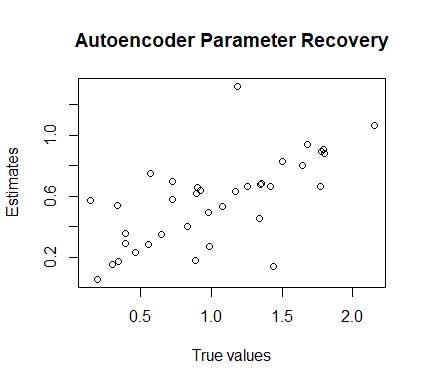
\includegraphics[width=\textwidth]{img/aied_results/ae_a_corr.png}
   \endminipage\hfill
   \minipage{0.5\textwidth}
   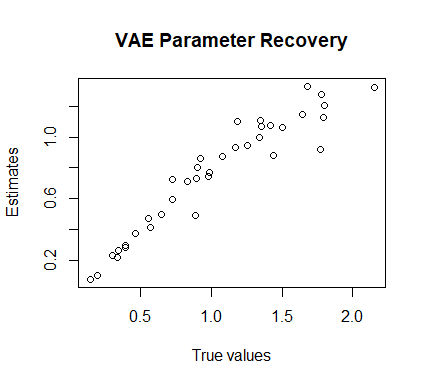
\includegraphics[width=\textwidth]{img/aied_results/vae_a_corr.png}
   \endminipage\hfill
   \caption{Autoencoder and VAE discrimination parameter ($a_{ik}$) recovery.}
   \label{fig:vae_vs_ae_a}
\end{figure}
\begin{figure}[h!]
\minipage{0.5\textwidth}
   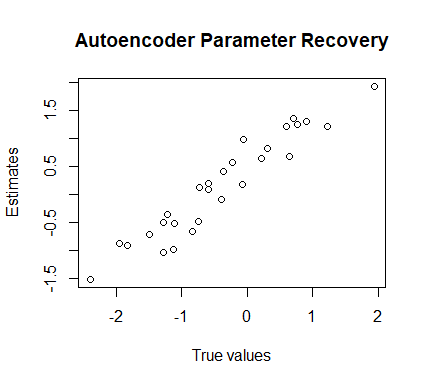
\includegraphics[width=\textwidth]{img/aied_results/ae_b_corr.png}
   \endminipage\hfill
   \minipage{0.5\textwidth}
   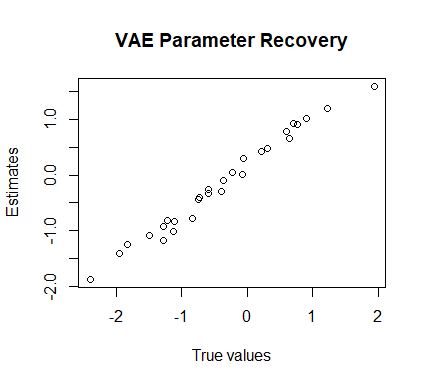
\includegraphics[width=\textwidth]{img/aied_results/vae_b_corr.png}
   \endminipage\hfill
   \caption{Autoencoder and VAE difficulty parameter ($b_i$) recovery.}
   \label{fig:vae_vs_ae_b}
\end{figure}

Results for student ability parameter estimates are shown in Table \ref{tab:vae_vs_ae_theta} and Figure \ref{fig:vae_vs_ae_theta}. Again, we see that the error measures from VAE estimates are much lower than those from a regular AE. However, the correlation values are slightly better for AE, though the difference is not visible in the correlation plot. The reason that AE has poor AVRB and RMSE measures is because the ability parameter estimates are on a different scale than the true values. Notice in the left plot of Figure \ref{fig:vae_vs_ae_theta} that the vertical axis reaches over $4$, while the vertical axis of right plot has closer range to the true scale of $\vect \Theta$. This is likely due to the KL-divergence term in the VAE loss function, better controlling the scale of the latent distribution to be near $\mathcal{N}(0,I)$.

\begin{table}[h!]
\centering
\begin{tabular}{ccccc}
\hline
Model & $\theta_1$ & $\theta_2$ & $\theta_3$ & Statistic \\
\hline
AE &  7.425 & 3.107 & 16.260 & AVRB \\
VAE   & 1.844 & 1.713 & 4.009 &  \\
\hline
AE & 1.788 & 1.523 & 1.746 & RMSE \\
VAE   & 0.664 & 0.760 & 0.646 & \\
\hline
AE & 0.970 & 0.937 & 0.971 & CORR \\
VAE   & 0.965 & 0.940 & 0.969 & \\
\hline
\end{tabular}
\caption{Error measures for latent trait prediction of AE and VAE.}
\label{tab:vae_vs_ae_theta}
\end{table}

The lack of a KL-divergence term in a regular AE also helps explain the poor discrimination parameter estimates shown in the right plot of Figure \ref{fig:vae_vs_ae_a}. The ML2P model can suffer from an identifiability issue without the assumption that student ability parameters follow some probability distribution \cite{ets2005}. Fixing this problem often requires an anchoring or rotation procedure after estimation \cite{baker_kim2004}. For a VAE, this is avoided by incorporating the KL-divergence term in Equation \ref{eq:vae_loss} between the encoder output and the prior distribution $p_\theta^*(\vect \Theta) = \mathcal{N}(0,I)$.

\begin{figure}[h!]
\minipage{0.5\textwidth}
   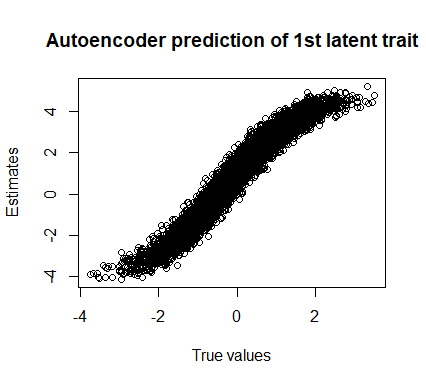
\includegraphics[width=\textwidth]{img/aied_results/ae_theta1_corr.png}
   \endminipage\hfill
   \minipage{0.5\textwidth}
   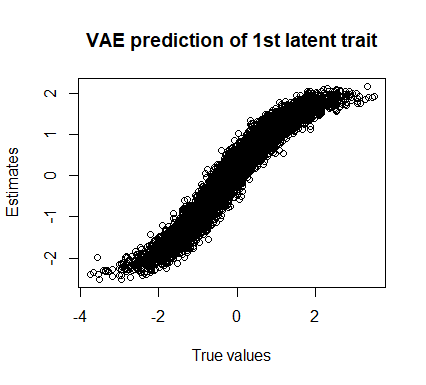
\includegraphics[width=\textwidth]{img/aied_results/vae_theta1_corr.png}
   \endminipage\hfill
   \caption{Autoencoder and VAE predictions for $\theta_1$.}
   \label{fig:vae_vs_ae_theta}
\end{figure}

Both autoencoders and variational autoencoders can be used as IRT parameter estimation methods when a $Q$-matrix restricts weights in the decoder. In either case, adding interpretability to neural networks is interesting, but a VAE is able to incorporate an extra piece of domain knowledge in the prior distribution of $\vect \Theta$, leading to more accurate estimates. The results presented in this section demonstrate the advantage that the ML2P-VAE method holds over the regular autoencoder architecture proposed by Guo et al. \cite{guo2017}.


\subsection{ML2P-VAE vs Traditional Methods}\label{sec:ml2pvae_compare}
In this section, a direct comparison of ML2P-VAE with traditional parameter estimation techniques for IRT. Three variants of ML2P-VAE are used: ML2P-VAE$_{full}$, ML2P-VAE$_{est}$, and ML2P-VAE$_{ind}$ as described in Section \ref{sec:variants}. These are compared against Metropolis-Hastings Robbins-Monro (MHRM) \cite{cai2009}, Quasi Monte-Carlo Expectation Maximization (QMCEM) \cite{mirt}, and Monte-Carlo Expectation Maximization (MCEM) \cite{bock1981}. This work has been published in the journal \textit{Machine Learning} \cite{ml_paper}.

A summary of each method's performance is given in Table \ref{tab:ml2p_results}. All experiments were conducted using Tensorflow for R on a laptop computer with a 2.9 GHz Intel Core i7-7500U CPU. Note that although artificial neural networks benefit greatly from GPU, we do not utilize this hardware and still get a sizable speedup in comparison to other methods. The results from traditional methods were obtained using default settings of the MIRT package \cite{mirt}. 

In all variations of ML2P-VAE, we train the neural network with the Adam optimizer \cite{adam} for 10 epochs and batch size 1 (pure stochastic gradient descent). The specific encoder architecture of the neural network was dependent on the size of the data set. Sim-6 used two hidden layers of size 32 and 16, ECPE used two hidden layers of 16 and 8 nodes, and Sim-20 utilized two hidden layers of size 64 and 32. In each network, a sigmoid activation function was used in the encoder hidden layers and a linear activation function in the encoded distribution. As described earlier, the ML2P-VAE model requires the use of a sigmoidal activation function in the output layer of the decoder.

\begin{sidewaystable}
\footnotesize{
\centering
\begin{tabular}{c|c|ccc|ccc|ccc|c}
  \hline
    Data Set & Method & $\vect a$.RMSE & $\vect a$.BIAS & $\vect a$.COR & $\vect b$.RMSE & $\vect b$.BIAS & $\vect b$.COR &  $\vect \Theta$.RMSE & $\vect \Theta$.BIAS & $\vect \Theta$.COR & Runtime \\
    \hline
& MHRM & 0.0693 & 0.0319  & 0.9986   & 0.0256 & -0.0021 & 0.9999  & 0.714  & -0.0033  & 0.7006 & 1110s \\ 
(i)& QMCEM & 0.149 & -0.067 & 0.9939 & 0.0376 & -0.002 & 0.9998 & 0.7206 & 0.0023 & 0.6939 & 322s\\
6 abilities& MCEM & 0.1497 & -0.0633 &  0.9936 &  0.0383 & 0.0035 & 0.9997 &  0.7206 & -0.0016 & 0.6938 & 1009s\\
Sim-6& ML2P-VAE$_{full}$ & 0.0705 &  0.0255  & 0.9985   & 0.0471 & -0.0079 & 0.9996  & 0.6649   & -0.0178  & 0.7476 & 343s\\
& ML2P-VAE$_{est}$ & 0.1803 & 0.0871  & 0.9891 &  0.064 & -0.0131 & 0.9993  & 0.7109 &  0.0772  & 0.7082 & 364s \\
& ML2P-VAE$_{ind}$ & 0.1218 & -0.0004 & 0.9944   & 0.0597 & -0.0145 & 0.9994  & 0.7222 &  0.0316  & 0.6928 & 252s\\
\hline 
& MHRM* & 0* & 0*&  1* &  0* &  0* &  1* & 0* & 0* &  1* & 162s \\
(ii)& QMCEM & 0.0159  & 0.0035 & 0.9999 & 0.0067  & -0.0005 & 1   & 0.0111 & 0.0007 & 0.9999 & 33s\\
3 abilities & MCEM & 0.0228 & 0.0148 & 0.9998 & 0.0064  & -0.0008 & 1   & 0.0132 & 0.0026 & 0.9998 & 192s \\
ECPE & ML2P-VAE$_{full}$ & N/A & N/A & N/A & N/A & N/A & N/A & N/A & N/A & N/A & N/A  \\
& ML2P-VAE$_{est}$ & 0.2794 & 0.2152 & 0.9713 & 0.148 & 0.0951  & 0.993 & 0.443 & -0.0628 & 0.8237 & 61s  \\
& ML2P-VAE$_{ind}$ & 0.3208 & 0.2184 & 0.9504 & 0.154 & 0.0872  & 0.9932  & 0.3063 & 0.01 & 0.9017 & 49s \\
\hline
& MHRM & N/A & N/A & N/A & N/A & N/A & N/A & N/A & N/A & N/A & N/A  \\
(iii)& QMCEM & N/A & N/A & N/A & N/A & N/A & N/A & N/A & N/A & N/A & N/A \\
20 abilities & MCEM & N/A & N/A & N/A & N/A & N/A & N/A & N/A & N/A & N/A & N/A  \\
Sim-20 & ML2P-VAE$_{full}$ & 0.078 &  0.0473  & 0.9983  & 0.0608 &  0.0054  & 0.9996  & 0.6145 &  0.0065  & 0.7893 & 1292s \\
& ML2P-VAE$_{est}$ & 0.2992  & -0.1304  & 0.9822  & 0.1655 &  0.1215  & 0.9987  & 0.7364   & -0.0276  & 0.7257 & 961s \\
& ML2P-VAE$_{ind}$ & 0.2043 &   0.0592  & 0.9792  & 0.0958   & -0.0029  & 0.9992  & 0.7054 &  0.0747  & 0.7135 & 850s \\
\hline 
        & MHRM & 0.0953 & -0.0158	&	0.9966 & 0.0614 & -0.0101 &	0.9988 & 0.6325	& 0.0118	& 0.7697 & 94s \\
        (iv)& QMCEM & 0.0938 & -0.0160	&	0.9967 & 0.0614 & -0.0179 &	0.9989 & 0.6326	& 0.0154	& 0.7696 & 29s \\
        4 abilities & MCEM & 0.0951 & -0.0138	&	0.9966 & 0.0644 & -0.0199 &	0.9987 & 0.6326	& 0.0150	& 0.7696 & 196s \\
       Sim-4 & ML2P-VAE$_{full}$ & 0.1326 & 0.0780		&	0.9960 & 0.0872 & -0.0311 &	0.9978 & 0.6384	& 0.0210	& 0.7648 & 37s \\
        & ML2P-VAE$_{est}$ & 0.2526 & 0.2106		&	0.9883 & 0.1035 & -0.0337 &	0.9980 & 0.6897	& -0.0256 	& 0.7182 & 38s \\
        & ML2P-VAE$_{ind}$ & 0.1658 & 0.1099		&	0.9939 & 0.0944 & -0.0254 &	0.9976 & 0.6474	& -0.0397	& 0.7579 & 30s \\

\hline
\end{tabular}
\caption{Error measures for discrimination ($\vect a$), difficulty ($\vect b$), and ability ($\vect \Theta$) parameters from various parameter estimation methods on three different data sets. Note that in the ECPE data set, there are no true values, so MHRM estimates are accepted as true. In Sim-20, only ML2P-VAE methods are capable of estimating such high-dimensional latent traits.}
  \label{tab:ml2p_results}
}
\end{sidewaystable}

Note that when comparing error measures in Sim-6, the ML2P-VAE methods are competitive with traditional methods. In particular, assuming full knowledge of the latent trait covariances in ML2P-VAE yields discrimination, difficulty, and ability parameter estimates of similar accuracy to MHRM. When the assumption of known latent trait correlation is relaxed, the accuracy of parameter estimates understandably slip.

Although the ML2P-VAE methods are slightly less accurate than MHRM, they are much faster than traditional methods, especially as the number of latent traits increase. Much of this speedup is due to the fact that neural networks do not require numerical integration over the latent abilities, and instead use simple hidden neural layers. While quadrature or MCMC methods become infeasible on data sets any larger than Sim-6, this is no cause for concern with ML2P-VAE. Note that for neural networks of this size (50-200 inputs and latent dimension 6-20), the longer runtime is more due to the number of data samples, rather than the size of the latent dimension. The affect of data size on runtime and accuracy is explored further in Section \ref{sec:data_size}. In fact, the largest neural network we used in these experiments, used on Sim-20, only had 1,670 trainable parameters, which is very small when compared to ANN models used for image classification or natural language processing. 

\begin{figure}[h]
\centering
\figuretitle{Discrimination Parameter Estimates}\\
    \begin{subfigure}{.32\textwidth}
      \centering
      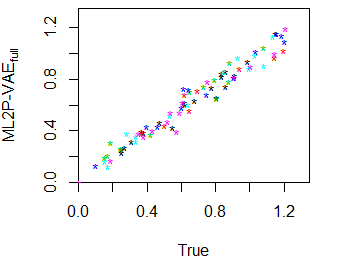
\includegraphics[width=.9\linewidth]{img/ml_journal_results/6skills/vae_full_disc_6skills.png}
    \end{subfigure}
    \begin{subfigure}{.32\textwidth}
      \centering
      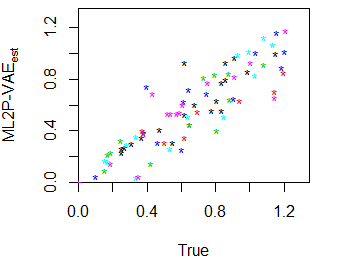
\includegraphics[width=.9\linewidth]{img/ml_journal_results/6skills/vae_est_disc_6skills.png}
    \end{subfigure}
    \begin{subfigure}{.32\textwidth}
      \centering
      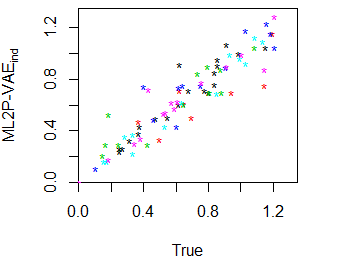
\includegraphics[width=.9\linewidth]{img/ml_journal_results/6skills/vae_ind_disc_6skills.png}
    \end{subfigure}
    \begin{subfigure}{.32\textwidth}
      \centering
      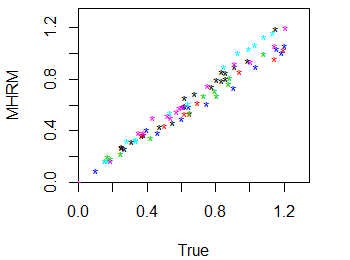
\includegraphics[width=.9\linewidth]{img/ml_journal_results/6skills/mhrm_disc_6skills.png}
    \end{subfigure}
    \begin{subfigure}{.32\textwidth}
      \centering
      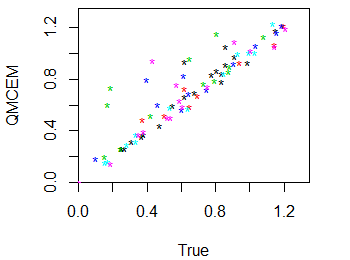
\includegraphics[width=.9\linewidth]{img/ml_journal_results/6skills/qmcem_disc_6skills.png}
    \end{subfigure}
    \begin{subfigure}{.32\textwidth}
      \centering
      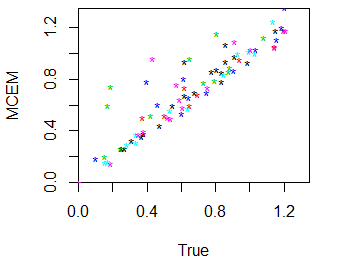
\includegraphics[width=.9\linewidth]{img/ml_journal_results/6skills/mcem_disc_6skills.png}
    \end{subfigure}
    \caption{Correlation plots of discrimination parameter estimates for the Sim-6 dataset with 50 items and 6 latent traits. ML2P-VAE estimates are on the top row, and traditional method estimates are on the bottom row.}
    \label{fig:6skill_cor}
\end{figure}

Some of the results are visualized in Figures \ref{fig:6skill_cor}, \ref{fig:ecpe_cor}, \ref{fig:20skill_cor}, and \ref{fig:4skills_disc} for Sim-6, ECPE, Sim-20, and Sim-4 respectively. Each color in the plots corresponds to a particular latent ability associated with the ability or discrimination parameter. For example, all red points correspond with estimates to $\theta_1$ or $\vect a_{:1}$. Figure \ref{fig:6skill_cor} shows the correlation between the true and estimated discrimination parameters for the ML2P-VAE$_{full}$ and MHRM methods. We don't include such plots for the difficulty parameters, as all methods estimate each $b_i$ with very high accuracy. From these figures, it appears that while MHRM obtains better results on smaller discrimination parameters, ML2P-VAE$_{full}$ has less error on larger parameters, and the estimation error seems to be independent of the magnitude of the parameter. The other two ML2P-VAE methods, ML2P-VAE$_{est}$ and ML2P-VAE$_{ind}$, do not reach the same levels of accuracy as when assuming full knowledge of the latent ability correlations. 

\begin{figure}[h]
\centering
    \begin{subfigure}{.32\textwidth}
      \centering
      \figuretitlesmall{Discrimination Parameters}
      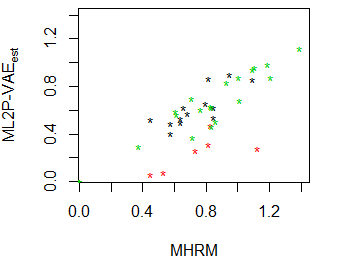
\includegraphics[width=.9\linewidth]{img/ml_journal_results/ecpe/vae_est_disc_ecpe.png}
    \end{subfigure}
    \begin{subfigure}{.32\textwidth}
      \centering
      \figuretitlesmall{Difficulty Parameters}
      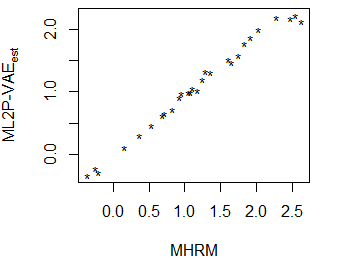
\includegraphics[width=.9\linewidth]{img/ml_journal_results/ecpe/vae_est_diff_ecpe.png}
    \end{subfigure}
    \begin{subfigure}{.32\textwidth}
      \centering
      \figuretitlesmall{Ability Parameters}
      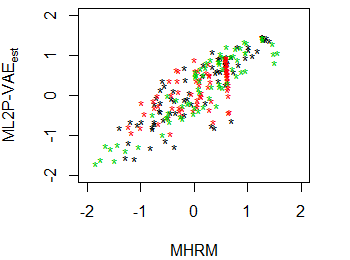
\includegraphics[width=.9\linewidth]{img/ml_journal_results/ecpe/vae_est_theta_ecpe.png}
    \end{subfigure}
    \begin{subfigure}{.32\textwidth}
      \centering
      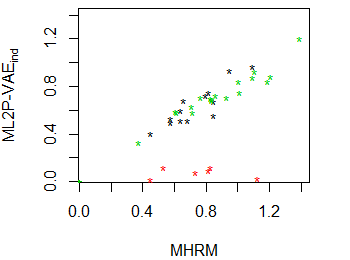
\includegraphics[width=.9\linewidth]{img/ml_journal_results/ecpe/vae_ind_disc_ecpe.png}
    \end{subfigure}
    \begin{subfigure}{.32\textwidth}
      \centering
      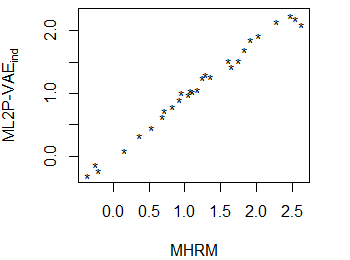
\includegraphics[width=.9\linewidth]{img/ml_journal_results/ecpe/vae_ind_diff_ecpe.png}
    \end{subfigure}
    \begin{subfigure}{.32\textwidth}
      \centering
      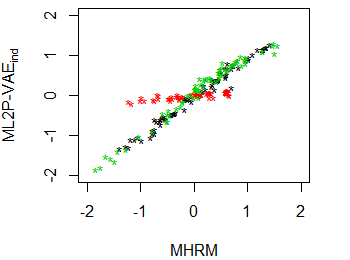
\includegraphics[width=.9\linewidth]{img/ml_journal_results/ecpe/vae_ind_theta_ecpe.png}
    \end{subfigure}
    \caption{Estimates from ML2P-VAE methods plotted against ``accepted'' MHRM estimates from the ECPE dataset.}
    \label{fig:ecpe_cor}
\end{figure}

When examining the ECPE data, there are no ``true'' values of parameters so ML2P-VAE's results are directly compared with MHRM's estimates. As seen in Table \ref{tab:ml2p_results}, the parameter estimates from QMCEM and MCEM are nearly identical to those of MHRM on the ECPE data. Of course, there is not a known covariance matrix between the three latent abilities, so only ML2P-VAE$_{est}$ and ML2P-VAE$_{ind}$ can be analyzed. While both methods perform similar to MHRM in difficulty parameter estimates, we can see that the two yield different results when applied to discrimination and ability parameters. 

First note that while ML2P-VAE$_{ind}$ gives accurate estimations for the green and black abilities (and the discrimination parameters associated with those abilities), the red ability estimates are all very near zero for every student. This tells us that the ML2P-VAE$_{ind}$ method found that the red ability has no effect on exam performance. On the other hand, ML2P-VAE$_{est}$ captures the general trend of the MHRM ability  parameters, but the estimates have much more variance. The discrimination parameter estimates also show some correlation, but each of the three abilities are on a different scale. This highlights the importance of developing better methods of estimating the latent trait correlations.
\begin{figure}[h]
\centering
\figuretitle{Discrimination and Ability Parameter Estimates}\\
    \begin{subfigure}{.32\textwidth}
      \centering
      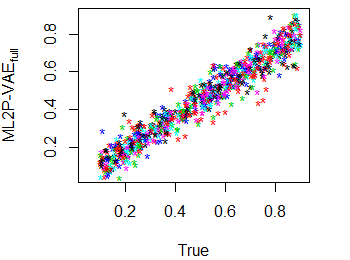
\includegraphics[width=.9\linewidth]{img/ml_journal_results/20skills/vae_full_disc_20skills.png}
    \end{subfigure}
    \begin{subfigure}{.32\textwidth}
      \centering
      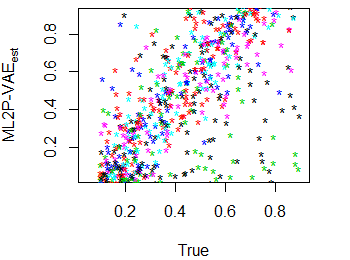
\includegraphics[width=.9\linewidth]{img/ml_journal_results/20skills/vae_est_disc_20skills.png}
    \end{subfigure}
    \begin{subfigure}{.32\textwidth}
      \centering
      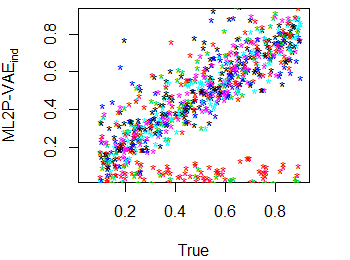
\includegraphics[width=.9\linewidth]{img/ml_journal_results/20skills/vae_ind_disc_20skills.png}
    \end{subfigure}
    \begin{subfigure}{.32\textwidth}
      \centering
      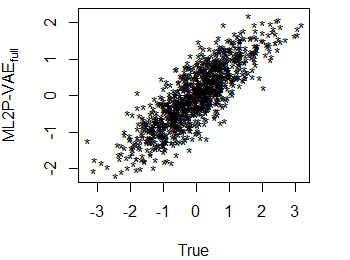
\includegraphics[width=.9\linewidth]{img/ml_journal_results/20skills/vae_full_theta_20skills.png}
    \end{subfigure}
    \begin{subfigure}{.32\textwidth}
      \centering
      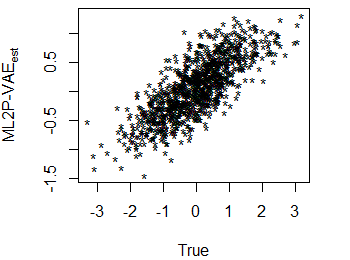
\includegraphics[width=.9\linewidth]{img/ml_journal_results/20skills/vae_est_theta_20skills.png}
    \end{subfigure}
    \begin{subfigure}{.32\textwidth}
      \centering
      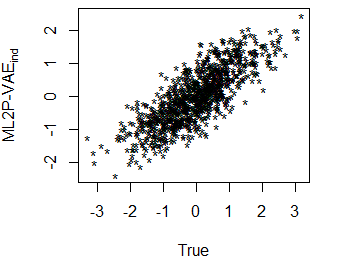
\includegraphics[width=.9\linewidth]{img/ml_journal_results/20skills/vae_ind_theta_20skills.png}
    \end{subfigure}
    \caption{ML2P-VAE parameter estimates for Sim-20 with 200 items and 20 latent traits. The top row shows discrimination parameter correlation, and the bottom row shows ability parameter correlation.}
    \label{fig:20skill_cor}
\end{figure}

While estimating parameters for the Sim-20 dataset, the dimension of the latent traits ($\R^{20}$) is too large for traditional methods to handle, so only the three ML2P-VAE techniques are studied. All three of these methods estimate the difficulty parameters with high accuracy. Similar to in Sim-6, it is again observed that the ML2P-VAE$_{full}$ error seems to be independent of the size of the discrimination parameter, a promising trend. However, ML2P-VAE does not perform as well when full knowledge of the latent ability correlation matrix is unknown. At first glance, the discrimination parameter estimates for ML2P-VAE$_{est}$ seem to have no pattern. But upon closer inspection, it can be seen that the discrimination parameter estimates associated with a particular ability (a particular color) are correlated, but each ability is on a different scale. 

The discrepancy between ML2P-VAE$_{full}$ and ML2P-VAE$_{est}$ can be attributed to a poorly estimated covariance matrix. For this data set, the covariance matrix obtained by the method described previously greatly overestimates every correlation between latent traits: the average signed bias $\sigma - \hat \sigma$ in the correlation matrix estimation computed using Equation \ref{eq:approx_cor_mat} is $-0.61$, and even the closest correlation estimation has signed bias $-0.26$. Finding a better method to compute an approximate correlation matrix could greatly improve ML2P-VAE$_{est}$.

The estimates for the Sim-20 dataset produced by ML2P-VAE$_{ind}$ display the same behavior observed in the ECPE dataset. Two of the abilities have discrimination parameters estimated near zero, meaning ML2P-VAE$_{ind}$ deemed these abilities to have no relation with performance on the assessment. But in contrast to the ECPE data, Sim-20 was simulated and so it is known that this is not true. Outside of this issue, the other discrimination parameters were reasonably estimated, showing clear correlation with the true values on near a 1:1 scale.

Though ML2P-VAE$_{est}$ and ML2P-VAE$_{ind}$ have trouble converging to the true discrimination parameters, they are still able to obtain quality estimates to the ability parameters. The values in Table \ref{tab:ml2p_results} for $\vect \Theta$ in Sim-20 are comparable to those of Sim-6. The plots in Figure \ref{fig:20skill_cor} show this high correlation in all three ML2P-VAE variants.

\begin{figure}[h]
\centering
\figuretitle{Discrimination Parameter Estimates}\\
    \begin{subfigure}{.32\textwidth}
      \centering
      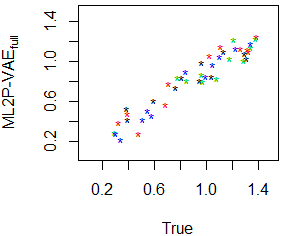
\includegraphics[width=.9\linewidth]{img/ml_journal_results/4skills/vae_full_disc_4skills_cropped.png}
    \end{subfigure}
    \begin{subfigure}{.32\textwidth}
      \centering
      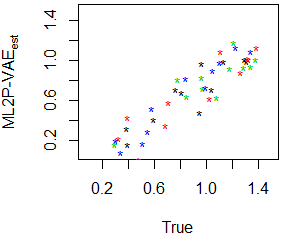
\includegraphics[width=.9\linewidth]{img/ml_journal_results/4skills/vae_est_disc_4skills_cropped.png}
    \end{subfigure}
    \begin{subfigure}{.32\textwidth}
      \centering
      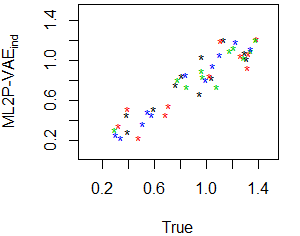
\includegraphics[width=.9\linewidth]{img/ml_journal_results/4skills/vae_ind_disc_4skills_cropped.png}
    \end{subfigure}
    \begin{subfigure}{.32\textwidth}
      \centering
      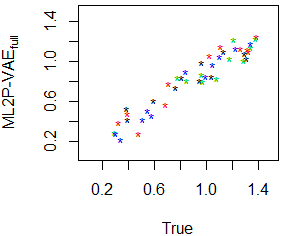
\includegraphics[width=.9\linewidth]{img/ml_journal_results/4skills/vae_full_disc_4skills_cropped.png}
    \end{subfigure}
    \begin{subfigure}{.32\textwidth}
      \centering
      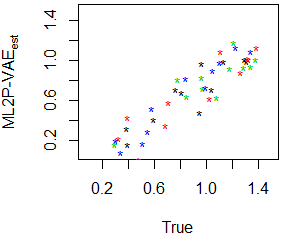
\includegraphics[width=.9\linewidth]{img/ml_journal_results/4skills/vae_est_disc_4skills_cropped.png}
    \end{subfigure}
    \begin{subfigure}{.32\textwidth}
      \centering
      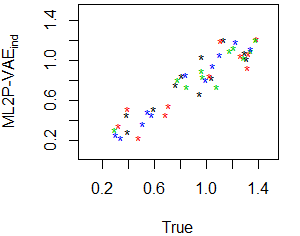
\includegraphics[width=.9\linewidth]{img/ml_journal_results/4skills/vae_ind_disc_4skills_cropped.png}
    \end{subfigure}
    \caption{Discrimination parameter estimates for Sim-4 with 27 items and 4 latent skills. The top row shows estimates from ML2P-VAE methods, and the bottom row gives estimates yielded by traditional methods.}
    \label{fig:4skills_disc}
\end{figure}

In the Sim-4 dataset, the advantages of ML2P-VAE methods are less apparent. The runtime difference is much smaller, since traditional methods do not struggle so much when integrating over a smaller latent dimension of size 4. This also affects the accuracy of parameter estimates. The latent skill estimates are better in Sim-4 than those of data set Sim-6 for all methods, but particularly the traditional methods. For latent abilities $\vect \Theta$ and difficulty of items $\vect b$, all six methods produced similar estimates, and so these correlation plots are omitted. As seen in Table \ref{tab:ml2p_results}, the corresponding error measures are very close, though traditional methods are slightly more accurate.

A comparison between the Sim-4 discrimination parameter estimates is shown in Figure \ref{fig:4skills_disc}, which clearly visualizes the values in Table \ref{tab:ml2p_results}. Though all ML2P-VAE methods produce highly correlated estimates, they also tend to underestimate the true values. This is most apparent in the plot for ML2P-VAE$_{est}$ and in the relative bias values in Table \ref{tab:ml2p_results}. While traditional parameter estimation results may be more desirable for the Sim-4 dataset, this demonstrates that the ML2P-VAE methods are most useful when the number of latent abilities is large.

\subsubsection{Effect of Training Data Size}\label{sec:data_size}
A common criticism of neural networks is that they are computationally intensive and training them with a gradient descent based algorithm (a first order method) can take a long time. They also require large amounts of data. As mentioned before, the architecture used in this application results in a relatively small neural network.

\begin{figure}[h]
\centering
    \begin{subfigure}{.47\textwidth}
      \centering
      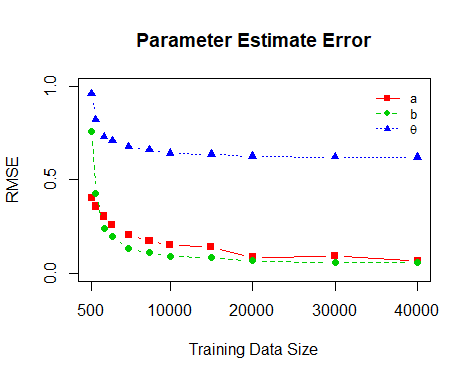
\includegraphics[width=\linewidth]{img/ml_journal_results/vae_full_train_size_error.png}
    \end{subfigure}
    \begin{subfigure}{.47\textwidth}
      \centering
      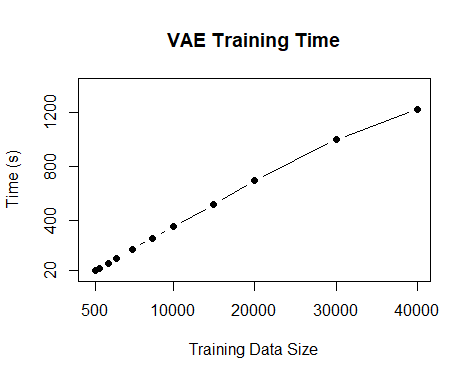
\includegraphics[width=\linewidth]{img/ml_journal_results/vae_full_train_size_time.png}
    \end{subfigure}
    \caption{Performance of ML2P-VAE$_{full}$ on data set (iii) when trained on data sets of increasing size. The left plot gives the test RMSE after using different sizes of training data, and the right plot shows the time required to train the neural network.}
    \label{fig:train_size}
\end{figure}

The longer runtimes in Table \ref{tab:ml2p_results} for Sim-20 can be attributed more to the fact that there were 50,000 data samples in the training set, rather than the large latent dimension. The left plot of Figure \ref{fig:train_size} displays the relation between the size of the training data and estimation accuracy. Error does not decrease very much after the number of training samples becomes greater than 20,000 -- less than half of the available simulated data. The right plot of Figure \ref{fig:train_size} shows that training time grows linearly with the size of training data. While this may seem obvious from the usual machine learning point of view, it is not always the case in parameter estimation. The main distinction here is that the size of the gradient vector for a neural network does not depend on the number of students $N$, while the gradient vector does grow with more students in traditional methods.

Both plots in Figure \ref{fig:train_size} demonstrate the trade-off between accuracy and speed, as well as highlighting that ML2P-VAE methods can still be viable even if the data size is not exceptionally large. This is particularly true in estimating the ability parameter $\vect \Theta$, whereas traditional methods are unable to estimate high-dimensional $\vect \Theta$. Estimating the difficulty parameters $\vect b$ is manageable with a smaller data set, while discrimination parameters require a large amount of training data to obtain quality estimates.


\section{Discussion}
\subsection{Future Extensions}\label{sec:ml2pvae_future}
The work described in this chapter introduces additional paths for continued research. One important topic involves analyzing the convergence of ML2P-VAE methods. It is important to find conditions which guarantee that the estimates for the discrimination and difficulty parameters will converge to their respective true values. Based on the results shown in Table \ref{tab:ml2p_results} and Figures \ref{fig:20skill_cor} and \ref{fig:ecpe_cor}, it seems likely that convergence will require full knowledge of the covariances among latent traits, since ML2P-VAE$_{full}$ performs much better than ML2P-VAE$_{est}$. In each data set, it is clear that either using an inaccurate estimated covariance matrix or simply assuming that latent traits are independent results in inaccurate parameter estimates. Another possible factor in ML2P-VAE's convergence is the sparsity of the $Q$-matrix. If $q_{ik} = 1$ for all $i,k$, then the connections between decoder layers seen in Figure \ref{fig:ml2pvae_visual} are unmodified, and interpretation of the encoded hidden layer as estimates to ability parameters and weights/biases in the decoder as discrimination/difficulty parameter estimates may not be possible.

In real applications, it is unlikely that the exact correlations between latent abilities are available, so an approximate covariance matrix would need to be used instead. The experiments in this work imply that convergence likely relies on knowledge of an accurate covariance matrix among latent traits, thus it is important to develop better methods of estimating this covariance matrix.

It is also possible that the ML2P-VAE method can be extended to estimating the parameters in the Multidimensional Logistic 3-Parameter model \cite{birnbaum1968}, which introduces a guessing parameter for each item. Implementing a guessing parameter into the VAE framework is trivial. However, since many other parameter estimation methods struggle in estimating a 3-parameter model \cite{baker_kim2004}, ``ML3P-VAE'' may face the same issue. Further work to extend ML2P-VAE architecture to the Samejima graded response model \cite{samejima1997} would allow for better analysis of student responses which are not recorded as a binary correct/incorrect. This also opens the door to other psychometric questionnaires where items are measured on a Likert scale \cite{likert1932}.

\subsection{Concluding Remarks}
ML2P-VAE is a novel unsupervised learning technique which allows IRT parameter estimation of correlated high-dimensional latent traits. This requires a VAE architecture capable of fitting a more general multivariate Gaussian distribution, rather than a standard normal distribution. Where other estimation methods rely on numerical integration or MCMC methods, which become infeasible for large numbers of latent abilities as described in Section \ref{sec:irt_est_background}, ML2P-VAE trains a neural network using a gradient descent based optimization method. Large datasets typically present a \textit{burden} to traditional IRT parameter estimation techniques, but big data is a \textit{blessing} to this deep learning-based approach.

While the ML2P-VAE method introduces hundreds or thousands of trainable parameters, the parameters in the decoder can be interpreted as estimates to discrimination and difficulty parameters. The individual parameters in the encoder do not represent anything concrete, but together, they learn a function which maps a student's response set to a distribution representing the student's latent ability.

All of these parameters are trained simultaneously by optimizing a single loss function. After training the neural network, the discrimination and difficulty parameter estimates are immediately available, and the ability parameter estimates are easily obtained at test time by feeding forward response sets through the encoder. Note that the estimates for $\vect \Theta_j$ are not directly trainable parameters of the neural network -- the partial derivatives $\displaystyle\frac{\partial \mathcal{L}}{\partial \theta_{jk}}$ are never calculated or directly optimized.

Of course, the most accurate ML2P-VAE method, ML2P-VAE$_{full}$, makes the strongest and most restrictive assumption; that the exact correlation quantities between latent abilities is known. This may be impractical in applications, and for this reason the other ML2P-VAE methods must also be closely examined. In theory, using a covariance matrix that is estimated from the data should yield better results than assuming all traits are independent. But if this estimated matrix is inadequate, the accuracy of parameter estimates suffers heavily. A possible way to remedy this is to adjust the weight of the KL-Divergence in the VAE loss function in Equation \ref{eq:vae_loss} by introducing a hyperparameter $\lambda$. Decreasing this hyperparameter ($\lambda < 1$) gives more emphasis on reconstructing inputs, rather than regularizing the data against an estimated distribution which may be flawed.

ML2P-VAE methods are most useful on high-dimensional data where traditional methods struggle. But even when applied to smaller data sets where traditional techniques are feasible, the results from ML2P-VAE are competitive. They are significantly faster in runtime, and yield similar error measures. When estimating difficulty parameters, the improvement gained from using traditional methods is incredibly small. Estimates for students' latent abilities are often more accurate when using ML2P-VAE methods, seen in Table \ref{tab:ml2p_results}. This is especially interesting, as the estimates $\vect \Theta_j$ are not updated in the iterations of a gradient descent algorithm, while the estimates to $a_{ik}$ and $b_i$ are. In all, these results show the versatility of ML2P-VAE methods in estimating item and ability parameters from a variety of data sets.



% Part II
\chapter{Time-Series Neural Networks and Knowledge Tracing}
\sideremark{TODO: explain why I have background on TSNN and KT here}
\sideremark{TODO: is ``Time-Series'' best to use? Maybe ``Temporal''?}

\section*{Time-Series Neural Networks}
In many deep learning applications such as video processing, natural language processing, or dynamical systems, the observed data is time-dependent \cite{kahou2015} \cite{vaswani2017} \cite{gilpin2020}.In such datasets, a single observation of $d$ features can not represented as a vector $\vect x_0 \in \R^d$, but must take into account the $T$ different measurements of the $d$ features, each taken at a different timestep $1 \leq t \leq T$. As such, a data point is represented as a matrix $X_0 \in \R^{d \times T}$, where each column $t$ of $X_0$ gives a snapshot of the observation at time $t$. 

\section{Recurrent Neural Networks}
Recurrent Neural Networks (RNN) are the most simple adaptation of neural networks to deal with time-series data. A regular feed-forward neural network layer takes an input vector $\vect x \in \R^d$ and outputs
\begin{equation}
  \vect y = f( W\vect x + \vect b)
  \label{eq:ffn_layer}
\end{equation}
where $W \in \R^{h \times d}$ and $\vect b \in \R^h$ are trainable parameters and $f$ is a non-decreasing activation function \cite{sharma2020}. 

In the time-dependent setting, let $\vect x_t$ be a column of an input $X$. A basic recurrent layer calculates 
\begin{equation}
  \begin{split}
    \vect h_t &= \tanh(W_{hh}\vect h_{t-1} + W_{hx}\vect x_t + \vect b_h) \\
    \vect y_t &= \sigma(W_{hy}[\vect x_t, \vect h_t] + \vect b_y)
\end{split}
  \label{eq:rnn_layer}
\end{equation}
where $W_{hh} \in \R^{h\times h}$, $W_{hx}\in \R^{h\times d}$, $\vect b_h \in \R^h$, $W_{hy} \in \R^{h \times (h+d)}$, and $\vect b_y \in \R^h$ are trainable parameters \cite{elman1990}. The notation $[\vect x_t, \vect h_t]$ refers to vector concatenation. Note that this allows the output $\vect y_t$ to include information from previous time-steps. A visualization of an unfolded RNN is shown in Figure \ref{fig:rnn_visual}.

\begin{figure}[h]
  \centering
  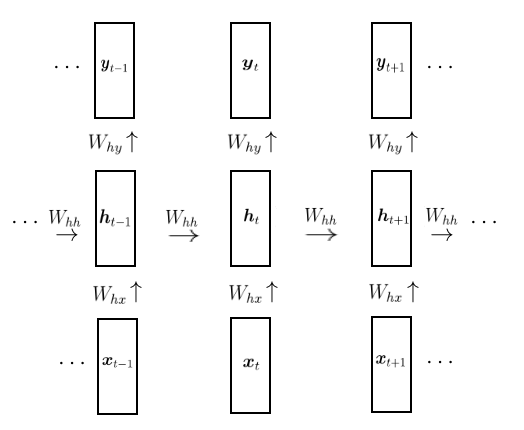
\includegraphics[width=.5\textwidth]{img/rnn_visual.png}
  \caption{Architecture of a recurrent neural network.}
  \label{fig:rnn_visual}
\end{figure}

One issue that RNN face is the exploding or vanishing gradient problem \cite{bengio1994}, where the norm of the gradient can become very large or very small during training. This is due to the fact that partial derivatives calculated during back-propagation between hidden states at time $t_1$ and $t_2$ is found by a product of $t_2 - t_1$ Jacobian matrices \cite{pascanu2013}. As the difference between $t_1$ and $t_2$ increases, the corresponding partial derivatives $\frac{\partial \vect h_{t_1}}{\partial \vect h_{t_2}}$ can exponentially grow or exponentially decay in norm.

Related to the exploding/vanishing gradient issue, RNN experience difficulty in retaining important information for multiple time-steps is difficult. For example, if an important phenomena happens to data point $X_0$ at time $t$, then that information should still influence the values of $\vect h_{t+10}$ and $\vect y_{t+10}$. But the structure described in Equation \ref{eq:rnn_layer} and Figure \ref{fig:rnn_visual} causes the impact of $\vect x_t$ and $\vect h_t$ to fade over time.


\section{Long Short-Term Memory Networks}
To combat this issue, Long Short-Term Memory (LSTM) networks were developed by Hochreiter and Schmidhuber \cite{hochreiter1997}. This architecture introduces element-wise multiplication and addition operations in addition to multiple trainable weights matrices which allows for tracking long-term dependencies. An LSTM layer computes a ``cell state'' vector $\vect c_t$, in addition to the hidden layer representation $\vect h_t$. This cell state is updated at each time-step to ``remember'' important information and ``forget'' frivolous information.

The LSTM structure also addresses the exploding/vanishing gradient of RNN. The presence of the cell state $\vect c_t$ ensures that calculating derivatives of long-range dependencies do not include many matrix multiplications \cite{hochreiter1997}.

A single cell of an LSTM can be compared to the middle block in Figure \ref{fig:rnn_visual} containing $\vect h_t$ of an RNN. At time $t$, given an input $t$ $\vect x_t$, previous hidden state $\vect h_{t-1}$, and previous cell state $c_{t-1}$, an LSTM cell uses four trainable weights matrices and four element-wise operations. First compute the ``forget'' vector $\vect f_t$, the ``update'' vector $\vect u_t$, the ``add'' vector $\vect a_t$, and the ``filter'' vector $\vect g_t$.
\begin{equation}
\begin{split}
  \vect f_t &= \sigma(W_f [\vect x_t, \vect h_{t-1}] + \vect b_f) \\
  \vect u_t &= \sigma(W_u [\vect x_t, \vect h_{t-1}] + \vect b_u) \\
  \vect a_t &= \tanh(W_a [\vect x_t, \vect h_{t-1}] + \vect b_a) \\
  \vect g_t &= \sigma(W_g [\vect x_t, \vect h_{t-1}] + \vect b_g)
\end{split}
  \label{eq:lstm_vects}
\end{equation}

The first three vectors in Equation \ref{eq:lstm_vects} are used to perform element-wise operations on $\vect c_{t-1}$ to produce the next cell state $\vect c_t$, and $\vect g_t$ is used in updating $\vect h_t$. Notice that the sigmoid activation function $\sigma(\cdot)$ maps small inputs to near $0$ and large inputs to near $1$, while the hyperbolic tangent activation function $\tanh(\cdot)$ maps small inputs to near $-1$ and large inputs to near $1$. 

Using $\vect f_t$, unimportant aspects (elements near zero) of $\vect c_{t-1}$ are forgotten:
\begin{equation}
  \vect c_{t-1}^* = \vect c_{t-1} \times \vect f_t
  \label{eq:lstm_forget}
\end{equation}
where $\times$ is element-wise multiplication. Next, $\vect u_t$ decides what information to update (elements near one), and $\vect a_t$ gives the value (an increase or decrease) of the information to be updated:
\begin{equation}
  \vect c_t = \vect c_{t-1}^* + \left( \vect u_t \times \vect a_t \right)
  \label{eq:lstm_update}
\end{equation}
where $+$ and $\times$ are element-wise addition and multiplication, respectively. Lastly, compute the next hidden state using $\vect g_t$, which filters the information to be passed to the next network layer and next time-step:
\begin{equation}
  \vect h_t = \tanh(\vect c_t) \times \vect g_t
  \label{eq:lstm_filter}
\end{equation}

\begin{figure}[h]
  \centering
  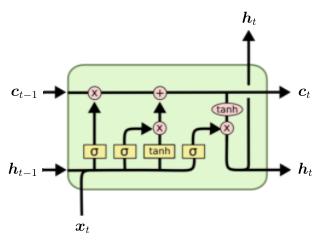
\includegraphics[width=.5\textwidth]{img/lstm_visual}
  \caption{Architecture of a single LSTM cell \cite{olah2015}. Trainable matrix multiplication followed by an activation function are in yellow boxes, and element-wise operations without learned parameters are in red ovals.}
  \label{fig:lstm_visual}
\end{figure}

The architecture of an LSTM is visualized in Figure \ref{fig:lstm_visual}. The forget vector acts as a gate which allows/disallows past information to persist over time, while the update and add vector grabs the data from the current input which is worth updating and remembering.


\section{Transformers and Attention}
Though LSTM networks presented a significant breakthrough in natural language processing (NLP), they have been quickly surpassed in the application of language modeling by attention-based methods. These models forgo the recurrent structure of information flow seen in RNN and LSTM for feed-forward layers and similarity scores between time steps. For example, calculating a similarity score between each pair of words in a sentence can help extract deeper context in language models such as transformers \cite{vaswani2017}.

While transformers are large neural networks with many components and parameters, they lean heavily on the attention mechanism. Given a $d$-dimensional feature vector $\vect x_t$ at each time-step $1\leq t\leq T$, define three trainable matrices $W_q$, $W_k$, and $W_v$. These are used to obtain a \textit{query}, \textit{key}, and \textit{value} vectors $\vect q_t$, $\vect k_t$, and $\vect v_t$ for each time-step. Note that these can be arranged into matrices $Q,K,V \in \R^{T\times d}$. Calculated the correlation between observation $t$ and all other time-steps:
\begin{equation}
  \vect c_t = \text{softmax}\left(\frac{K \vect q_t}{\sqrt{d}} \right) \in \R^T
  \label{eq:attn_cor}
\end{equation}


Notice that the matrix multiplication $K \vect q_t$ in Equation \ref{eq:attn_cor} is simply $T$ individual dot-product computations. So the $i$-th entry of $\vect c_t$ gives the similarity between the input at time $t$ and the input at time $i$. The softmax function $\text{softmax}(z_i) = \frac{e^{z_i}}{\sum_{j=1}^T e^{z_j}}$ rescales the dot product calculations so that the sum of the entries of $\vect c_t$ is equal to 1. In applications where an input $\vect x_{t_1}$ is not allowed to see information of future inputs $\vect x_{t_2}$, $t_1<t_2$, the corresponding entries of $K\vect q_{t_1}$ are masked to be $-\infty$. This causes the entries $c_{ti} = 0$ when $i > t$.

Next, the attention is calculated as 
\begin{equation}
  \vect a_t = V \vect c_t \in \R^d
  \label{eq:attn}
\end{equation}
The attention vector $\vect a_t$ is a weighted sum of the value vectors of each other time-step, weighted by the correlation scores in Equation \ref{eq:attn_cor}. The attention calculation can also be written more generally:
\begin{equation}
  A = \text{softmax}\left(\frac{QK^\top}{\sqrt{d}} \right) V \in \R^{T \times d}
  \label{eq:attn_matrix}
\end{equation}

In attention networks, the attention vectors $\vect a_t$ are individually sent through feed-forward layers. For example, transformers calculate attention and then use three feed-forward layers in a single ``block'' \cite{vaswani2017}. These blocks are stacked on top of each other up to six times to obtain deeper and deeper contextualization of the input sequence \cite{dai2019}. Eventually, this contextualization is plugged into a final prediction layer, depending on the application.

It should be pointed out that transformers and attention networks were developed for the NLP application. So in this case, a sequence of $T$ inputs represents a sentence of length $\leq T$ and an input vector $\vect x_t$ is a $d$-dimensional learned representation of an individual word \cite{mikolov2013}. Then the correlation score in Equation \ref{eq:attn_cor} is quantifying the relationship between pairs of words in the sentence.



\section*{Knowledge Tracing}
Knowledge Tracing (KT) is a task introduced by Corbett and Anderson in 1995 \cite{corbett1995}. Their goal was to model the changing knowledge state of students as they progress through an online intelligent tutoring program. This tutoring system helps students practice writing computer programs by testing them on various rules, such as correct use of in-built functions, and providing feedback on their mistakes. The model tracks each student's knowledge as being in either a learned or unlearned state for each rule. After each interaction, there is a probability $P(T)$ that a student makes the transition from the unlearned state to the learned state.

The probability that a student has learned a particular rule at timestep $n$ is
\begin{equation}
P(L_n) = P(L_{n-1} | \text{evidence}) + (1 - P(L_{_n-1} | \text{evidence})) \cdot P(T).
\label{eq:kt}
\end{equation}
Then the probability of a student performing a task correctly is the sum of the probability that the rule is learned and the student doesn't make a mistake, and the probability that the rule is unlearned but the student guesses correctly.

There are only four parameters for each rule: the probability that the rule is already in the learned state at timestep 0, the probability of transitioning from the unlearned to learned state, the probability of guessing correctly, and the probability of slipping. These parameters are estimated using a hidden Markov Model, and the probability of a student having learned a rule is updated via Bayes' Theorem.

In recent years, Bayesian Knowledge Tracing (BKT) has been overcome by deep learning methods. The popularity of neural networks has brought black-box models that yield high accuracy. Many of these methods, detailed in Section \ref{sec:kt_lit}, do not provide a concrete measure of student ability over time. Instead, the only way to track student knowledge is through the predicted probability of them answering questions correctly at a given timestep. 

In Chapter \ref{ch:kt_methods}, new methods using neural networks are presented which produce comparable predictive power to deep learning methods, while providing explainable models with links to Item Response Theory.


\section*{Knowledge Tracing Literature Review}\label{sec:kt_lit}
In the modern knowledge tracing application, data is provided as a sequence of student interactions $x_t = (q_t, c_t)$, $0 \leq t \leq L$. $L$ is a hyper-parameter denoting the maximum length of the sequence -- since the number of interactions for each student is different, response sequences shorter than $L$ are padded with null interactions, and response sequences of length longer than $L$ are wrapped into multiple sequences. For example, if $L=128$ and a particular student answers $160$ questions, then this student's interactions will be split into two separate sequences of length $128$ and $32$.

The tag $q_t$ indexes a particular question (item) in the available question bank, and $c_t \in\{0,1\}$ indicates whether the question was answered correctly or not. So for learning system with $n$ available questions, there are $2n$ possible interactions for $x_t$. The knowledge tracing task is to predict $c_{t+1}$ given all previous interactions. Mathematically, the quantity of interest is the probability 
\begin{equation}
  P(c_{t+1} = 1 | (q_0,c_0), (q_1,c_1),\ldots,(q_t, c_t), (q_{t+1}, ?)).
  \label{eq:kt_prob}
\end{equation}
Most neural networks optimize the predicted probability in Equation \ref{eq:kt_prob} by  minimizing the cross-entropy loss function, as described in Equation \ref{eq:cross_entropy}.

\section{Deep Knowledge Tracing}
In 2015, the first use of neural networks for knowledge tracing was introduced by Piech et al. \cite{piech2015}. Deep Knowledge Tracing (DKT) utilizes recurrent neural networks (RNN) and Long-Short Term Memory (LSTM) neural networks to predict a student's success on future questions, given a sequence of previous interactions. RNN are the most simple neural network to deal with sequential time-series data. LSTM are more sophisticated, and are capable of capturing longer-range dependencies due to their ``keep/forget'' functionality. %\sideremark{Do I need to give background on RNN and LSTM?} %TODO

Similar to natural language processing, tokens (student interactions) need to be represented as a $d$-dimensional vector. DKT does this by one-hot encoding the interactions in the input layer of shape $(2n+1, L)$,  and linearly mapping to a hidden layer of shape $(d, L)$. Each interaction in the sequence is treated independently in this layer. The input layer shape is $2n+1$ for each of the possible $2n$ interactions, along with space for an additional padding token representing a null interaction (for response sequences of length $< L$.

  The architecture of DKT is as follows: The one-hot encoding input layer, the $d$-dimensional embedding, an LSTM layer of size $d$, and a feed-forward output layer with $n$ nodes. The final layer uses a sigmoid activation function, and the output at each node represents the probability of answering that item correctly at the given timestep. To calculate loss, only the item tag for the next interaction and corresponding output node is used in the cross-entropy loss calculation.

  \section{Dynamic Key-Value Memory Networks}\label{sec:dkvmn}
More sophisticated neural network approaches to knowledge tracing were introduced by Zhang et al. with Dynamic Key-Value Memory Networks (DKVMN) \cite{zhang2017}. They modify a memory-augmented neural network (MANN) in order to fit into the knowledge tracing framework. A MANN is a time-series neural network, but it does not rely on residual connections like an RNN or LSTM. Rather, a value matrix $M^v$ is stored in memory for each student, and the entries in $M^v$ are updated in each timestep. The predicted output is a probability dependent on the previous value of $M^v$ in timestep $t-1$, as well as the current neural network input in timestep $t$.

In DKVMN, there is some added interpretability by requiring the number of columns of $M^v$ to be equal to the number of knowledge concepts $K$. In this way, the columns of $M^v$ offer an $h$-dimensional representation of the student's skill. DKVMN splits the computations into two parts: \textit{read} from $M^v$ to make a prediction, and \textit{write} to $M^v$ to update its information. The predictive part inputs only an exercise tag $q_t$ without the true response $c_t$. The question tag is linearly embedded into a vector $k_t$. $k_t$ is a representation of question $q_t$, and is then multiplied by a learned matrix $M^k$ and softmaxed. 

This creates a vector $w_t$, where entry $j$ in $w_t$ represents the correlation weight between the question $q_t$ and memory slot $j$. This process of taking the dot product between an item embedding and a trainable matrix and softmaxing is similar to the concept of ``attention'', used in popular NLP techniques such as transformers \cite{vaswani2017}.

Next, \textit{read} from the value matrix by computing 
\begin{equation}
  r_t = \sum_{i=1}^K w_t(i) M^v(i).
  \label{eq:dkvmn_read}
\end{equation}
Note that $r_t$ is simply a weighted sum of the columns of $M^v$ and can be treated as a summary of the student's predicted master level of exercise $q_t$. Next, the item embedding $k_t$ is appended to the read content $r_t$ and fed forward through two linear layers. The first uses a $\tanh$ activation function, and the output $p_t$ produced a single node and a sigmoidal activation. In this way, the single value $p_t$ represents the probability that the student will answer item $q_t$ correctly at that timestep.

The second part of DKVMN is to \textit{write} new values into $M^v$ based on the true response of students. Different from the prediction phase, the full tuple $(q_t,c_t)$ is embedded into a vector $v_t$. The manner in which $M^v$ is updated is actually similar to that of an LSTM, allowing for ``remembering'' and ``forgetting''. Two trainable matrices are multiplied by $v_t$ to produce an ``erase`` vector $e_t$ and an ``add`` vector $a_t$. The erase vector has a sigmoidal activation function, so that values near zero do not get erased much at all, and values near 1 get erased quite a bit. The add vector uses a $\tanh$ activation function, so memory slots in $M^v$ can either be increased or decreased. Finally, the columns of the memory matrix are updated via
\begin{equation}
  M_{t}^v(i) = (M_{t-1}^v(i) [1 - w_t(i) e_t] ) + w_t(i) a_t
  \label{eq:update_dkvmn}
\end{equation}
Note that the correlation weights $w_t$ computed in the predictive step are again used to determine \textit{how much} of memory slot $i$ should be updated.

%\sideremark{should I include image of DKVMN architecture?} %TODO

DKVMN's use of a matrix stored in memory allows for longer range dependencies than RNN or LSTM. There is also a bit of interpretability in this method, since a single column of the memory matrix $M_t^v$ gives an $h$-dimensional representation of a single skill for the student at time $t$. However, it cannot be determined \textit{which} skill the column represents. Additionally, if a student answers each available item, then stacking each weights vector $w_t$ into a matrix $W = \{w_t\}_{t=1}^L$ should result in a matrix similar to the item-skill association $Q$-matrix. But again, the columns of this ``learned $Q$-matrix'' $W$ are in no particular order, and can be difficult to interpret.

\subsection{Deep-IRT}
Deep-IRT, proposed by Chun-Kit Yeung \cite{yeung_2019} modifies the DKVMN architecture to allow a connection with Item Response Theory. Specifically, two separate feed forward layers are inserted, representing a student's $k$-th ability at time $t$ $\theta_{tk}$ and concept difficulty $\beta_k$. Then the output probability is not another linear layer (as in DVKVMN), but is instead a function of $\theta_{tk}$ and $\beta_k$:

\begin{equation}
  p_t = \frac{1}{1 + \exp\left( \beta_k - 3\cdot \theta_{tk} \right)}
  \label{eq:deep_irt_prob}
\end{equation}

These modifications provide a link to the Rasch model in Equation \ref{eq:rasch}. The multiplication by 3 is for practical reasons to re-scale $\theta_{tk}$. However, note that in Equation \ref{eq:deep_irt_prob}, the difficulty parameter is on the \textit{concept} level, and not the \textit{item} level like the Rasch model (and other IRT models). Though Deep-IRT doesn't seek to directly approximate the Rasch model, the modifications to DKVMN still adds significant interpretability to the deep neural network.


\section{Self-Attentive Knowledge Tracing}\label{sec:sakt}
In the field of natural language processing (NLP), the most state-of-the-art methods utilize a mechanism called self-attention \cite{vaswani2017}, which rely on calculating the correlation between pairs of words in a sentence. Popular models such as BERT \cite{bert} and GPT-3 \cite{gpt3} are both transformer-based neural networks for NLP which heavily depend on attention. Self-Attentive Knowledge Tracing (SAKT) adapts this concept for the knowledge tracing task \cite{pandey2019}. 

Similar to other deep learning methods, at timestep $t$, SAKT first embeds each interaction $(q_i, c_i)$, $i<t$ into a learned $d$-dimensional vector $m_i$. Additionally, like DKVMN, the current question $q_t$ without the response is also embedded into a $d$-dimensional vector $e_t$. 

The exercise embedding $e_t$ is multiplied by a weights matrix to obtain a \textit{query} vector $\vect q_t = W^{Q}e_t$. The interaction embedding $m_i$ is used to create two vectors: a \textit{key} vector $\vect k_i = W^{K}m_i$ and a \textit{value} vector $\vect v_i = W^V m_i$. 

The general idea is that $\vect k_i$ serves as the identifier of a past interaction, and $\vect q_t$ serves as an identifier for the current exercise. If the two exercises are similar in content, then the dot product between these two vectors should be large. The value vector $\vect v_i$ holds more abstract information about the corresponding interaction. The keys and values are organized into matrices $K$ and $V$. We calculate the attention
\begin{equation}
  a_{t} = \text{softmax}\left(\frac{K \vect q_t}{\sqrt{d}} \right) V
  \label{eq:attn_sakt}
\end{equation}

The value $\frac{K \vect q_t}{\sqrt{d}}$ yields a vector where each entry is the dot product between the current exercise query $\vect q_t$ and an interaction key $\vect k_i$. This is scaled by dimension and softmaxed, resulting in a weighted sum of the value vectors $\vect v_i$.

The attention value $a_t$ is sent through a few feed-forward layers, resulting in a vector $f_t = \text{FFN}(a_t)$. The output layer is $p_t = \sigma(f_t W + b)$, the probability that the student will answer the current exercise $q_t$ correctly.


\section{Performance Factors Analysis}
An earlier approach to knowledge tracing was proposed by Pavlik et al. in 2009 with Performance Factors Analysis (PFA) \cite{pavlik2009}. The general idea is that a student's learning at a given timestep is a function of the student's past interactions with items related to various knowledge concepts. Specifically, the logit of a student answering item $i$ correctly is a linear combination of concept difficulty, previous successes, and previous failures:
\begin{equation}
  p(j,k\in \text{K}_i, s, f) = \sigma\left(\sum_{k \in K}(\beta_k + \gamma_k s_{jk} + \rho_k f_{jk}\right)
  \label{eq:pfa}
\end{equation}

In Equation \ref{eq:pfa}, $\text{K}_i$ is a set indicating which knowledge concepts are required for item $i$, the trainable parameter $\beta_k$ represents concept $k$'s difficulty, and $\gamma_k$ and $\rho_k$ serve as trainable weights. $s_{jk}$ and $f_{jk}$ track the prior successes and failures, respectively, of student $j$ on concept $k$. At timestep $t$, we can write $s_{jk}$ and $f_{jk}$ as 
\begin{equation}
  \begin{split}
    s_{jk} = \sum_{i<t} \chi_{c_i=1} \cdot \chi_{k \in \text{K}_i} \\
    f_{jk} = \sum_{i<t} \chi_{c_i=0} \cdot \chi_{k \in \text{K}_i}
  \end{split}
  \label{eq:pfa_indicator}
\end{equation}
where $\chi$ is the indicator function on some condition. For example, $\chi_{k\in \text{K}_i}$ indicates whether the previous item $q_i$, $i<t$, required knowledge concept $k$ or not.

The parameters $\beta_k$, $\gamma_k$, and $\rho_k$ are learned so that they maximize the log-likelihood of the given dataset. This is a well-studied problem, as the form of Equation \ref{eq:pfa} is essentially just a logistic regression. Note that similar to Deep-IRT, PFA focuses on the concept-level, rather than item-level, parameters. 

\subsection{Deep Performance Factors Analysis}
Recent work has related PFA to the self-attention mechanism used in SAKT described in Section \ref{sec:sakt}. Pu et al. \cite{deep_pfa} developed Deep Performance Factors Analysis (DPFA) and a new characterization of the weight parameters $\gamma_k$ and $\rho_k$, using learned item embeddings $e_i$ for each question $q_i$.

For the current question $q_{t+1}$, the attention between previous exercises is $A_{i,t+1} = e_i^\top e_{t+1}$, for $i \leq t$. More recent interactions are taken into account by calculating $d_{i,t+1} = -a(t-i+1)+b$, where $a$ and $b$ are trainable parameters. Then the relevance of a past item depends on the dot product similarity and how long ago the interaction took place:
\begin{equation}
  w_i = \text{softmax}(A_{i,t+1} + d_{i,t+1})
  \label{eq:time_bias_attn}
\end{equation}

The mastery of knowledge concepts after a student completes interaction $(q_i, c_i)$ is given as $v_i = [v_i^0, v_i^1] \in \R^2$. The numbers $v_i^0$ and $v_i^1$ represent the expected mastery of the skills for item $i$ if the item is answered incorrectly or correctly, respectively. DPFA gives the probability of a student answering item $q_{t+1}$ correctly as
\begin{equation}
  p_{t+1} = \sigma\left( \beta_{t+1} + \sum_{i \leq t} \left( \chi_{c_i=0}\cdot w_i v_i^0 + \chi_{c_i=1} \cdot w_i v_i^1 \right) \right)
  \label{eq:dpfa}
\end{equation}
where $\beta_{t+1}$ corresponds to the difficulty of the current item and $\sigma(\cdot)$ is the sigmoid function. In comparison with regular PFA in Equation \ref{eq:pfa}, substitutes the terms $\chi_{c_i=0}\cdot w_i v_i^0$ for $\rho_k f_k$ and substitutes $\chi_{c_i=1} \cdot w_i v_i^1$ for $\gamma_k s_k$.

\chapter{Deep, Interpretable Methods for Knowledge Tracing} \label{ch:kt_methods}

The deep neural network approaches described in the previous section (including DKT, DKVMN, and SAKT) to the knowledge tracing problem have produced very high predictive power. Given a sequence of previous student interactions and a current question, they are capable of outputting the probability that the current question will be answered correctly with high accuracy. For the most part, this is the only metric produced by these models to measure student learning. But there already exists a theoretical framework for computing the probability of a correct response: Item Response Theory, introduced in Section \ref{sec:irt}.

In this section, we introduce an interpretable modification to deep knowledge tracing methods, published in the proceedings of AIED 2021 \cite{kt_irt}. Specifically, we link Item Response Theory models into the structure of knowledge tracing neural architecture. Besides the theoretical advantages this gives to a knowledge tracing model, it is also very helpful in practice. First, it provides an accessible and explicit representation of student knowledge at each timestep. This is an upgrade from other deep knowledge tracing methods, where the only meaningful values produced is $p_{t+1}$, the probability of answering the next question correctly (Equation \ref{eq:kt_prob}). The proposed modification also functions as a parameter estimation technique, quantifying the difficulty and discrimination power of items.

The connection between knowledge tracing and IRT has been explored before via Deep-IRT. The IRT-inspired knowledge tracing methods presented here differ from Deep-IRT in a few ways. First, Deep-IRT is tightly coupled with DKVMN, while the proposed method is readily applicable to a variety of deep knowledge tracing models. Our approach also allows for items to be associated with multiple skills, and directly emulates the ML2P model in Equation \ref{eq:ml2p} or the Rasch model in Equation \ref{eq:rasch} by producing estimates to discrimination and difficulty parameters. The focus here involves item-level parameters, rather than the concept-level parameters considered in Deep-IRT. The implementation details we use are completely different from that of Deep-IRT. Rather than adding separate networks for each parameter, we modify the output layer using information from the item-skill association $Q$-matrix, similar to the methodology of ML2P-VAE in Section \ref{sec:ml2p_vae}.

In this section, a trade-off is presented between predictive power and interpretability, but the proposed method remains competitive with other deep learning methods. While sacrificing a small amount of accuracy (measured by AUC), IRT-inspired knowledge tracing provides an explicit representation of student knowledge $\vect \Theta$ at each timestep. This representation of student knowledge is an upgrade from other deep knowledge tracing methods, which approximate skill mastery after the fact by averaging the probability of correctly answering all items associated with a particular skill. Additionally, parameters of the proposed modified neural network can be interpreted as approximations to the item parameters $a_{ik}$ and $b_i$ in Equation \ref{eq:ml2p}. In this sense, our proposed models function as both a knowledge tracing and a parameter estimation method.


\section{Incorporating IRT into Knowledge Tracing}
Given a tutoring system with $n$ available items, $K$ skills under assessment, and the skill association of each item given as a binary matrix $Q \in \{0,1\}^{n \times K}$ \cite{daSilva2018}, each of the possible $2n$ student interactions $(q_t, c_t)$ is represented as a learned $d$-dimensional vector $\vect x_t \in \mathbb{R}^d$. This can be done by multiplying a one-hot encoding of the $2n+1$ interactions (including a null/padding interaction) by a trainable $(2n+1) \times d$ matrix.

\sideremark{TODO: change image from ``time-series'' to ``temporal''}
\begin{figure}[h]
  \centering
  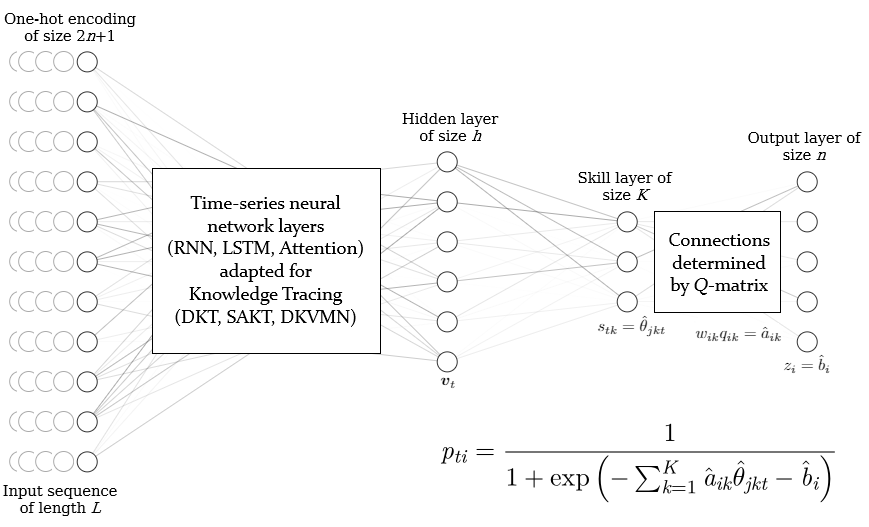
\includegraphics[width=.95\textwidth]{img/kt_irt/kt_irt_visual_with_equation_2.png}
  \caption{Visualization of integrating IRT into a knowledge tracing model with $L=4$, $n=5$, and $K=3$.}
  \label{fig:kt_irt_visual}
\end{figure}

Each student's response sequence includes $\vect x_0$, a null interaction to indicate the start of their interactions. A hyper-parameter $L$ is chosen indicating the maximum length of a student's response sequence. Interaction sequences shorter than $L$ are padded, and interaction sequences longer than $L$ are split into multiple sequences. A student's sequence of embedded interactions $\{\vect x_t\}_{t=0}^L$ is fed through a temporal neural network (TNN), such as an LSTM (similar to DKT \cite{piech2015}) or an attention-based model (similar to SAKT \cite{pandey2019}). This outputs an $h$-dimensional vector $\vect v_t$ for each interaction $\vect x_t$ in the input sequence.

\begin{equation}
  \vect v_t = \text{TNN}(\vect x_t, \vect x_{t-1}, \ldots, \vect x_0), \quad \vect v_t \in \R^h
  \label{eq:tsnn_layer}
\end{equation}

Next, each $\vect v_t$ is sent through a linear layer feed-forward network with output size $K$ (the number of latent concepts), yielding the skill vector $\vect s_t$.
\begin{equation}
  \vect s_t = W_s \vect v_t + \vect y, \quad W_s \in \R^{K\times h}, \vect y \in \R^K
  \label{eq:skill_layer}
\end{equation}
The weights matrix $W_s$ and bias vector $\vect y$ are trainable parameters. Each node in this ``skill layer'' represents a knowledge concept.

Finally, the output layer of the model has $n$ nodes and a sigmoid activation function $\sigma(\cdot)$, with each node representing the probability of the student answering that item correctly.

\begin{equation}
  \vect p_t = \sigma(W_p \vect s_t + \vect z) = \frac{1}{1 + \exp \left( -W_p \vect s_t - \vect z \right)}, \quad W_p \in \R^{n \times K}, \vect z \in \R^n.
  \label{eq:pred_layer}
\end{equation}
$W_p$ and $\vect z$ are trainable and importantly, $W_p$ is modified so that the nonzero values of $W_p$ are determined by the $Q$-matrix \cite{guo2017}\cite{ijcnn_paper}. If item $i$ does not require skill $k$, then the weight between the corresponding nodes is fixed to be zero. In this way, we write
\begin{equation}
  W_p \gets W_p \odot Q,
  \label{eq:weight_constraint}
\end{equation}
where $\odot$ is element-wise multiplication of matrices. Then the probability that the student will answer question $i$ correctly at timestep $t$ is given by 
\begin{equation}
  p_{ti} = \frac{1}{1 + \exp\left( -\sum_{k=1}^K w_{ik} q_{ik} s_{tk} - z_i \right)}
  \label{eq:nn_out}
\end{equation}
where $w_{ik}$, $q_{ik}$, $s_{tk}$, and $z_i$ are entries in $W_p$, $Q$, $\vect s_t$, and $\vect z$, respectively.

This constraint allows for interpretation of the final neural network layers as an approximate ML2P model: note the similarity between Equation \ref{eq:nn_out} and Equation \ref{eq:ml2p}. A visualization of this proposed neural network architecture is seen in Figure \ref{fig:kt_irt_visual}.

%\begin{figure}[h]
%  \centering
%  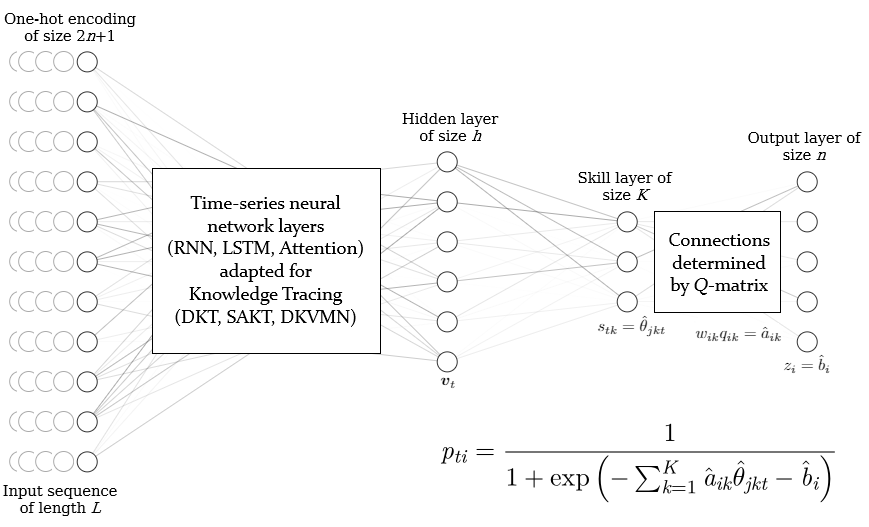
\includegraphics[width=.95\textwidth]{img/kt_irt/kt_irt_visual_with_equation_2.png}
%  \caption{Visualization of integrating IRT into a knowledge tracing model with $L=4$, $n=5$, and $K=3$.}
%  \label{fig:kt_irt_visual}
%\end{figure}

The weights between the skill and output layer $(w_{ik}q_{ik})$ serve as estimates to the discrimination parameters $a_{ik}$, and the bias parameters in the output layer $z_i$ are estimates to difficulty parameters $b_i$. The student's $k$-th latent ability $\theta_k$ is estimated at timestep $t$ via $s_{tk}$. This presents a clear analogue with ML2P-VAE, but the method described in this section makes no assumption about the prior distribution of latent traits $\vect \Theta$ -- there is no KL-Divergence term in the knowledge tracing loss function. In this way, IRT-inspired knowledge tracing is more similar to the modified autoencoder proposed by Guo et al. \cite{guo2017} and described in Section \ref{sec:ae_v_vae_results}.


\chapter{Comparison of Knowledge Tracing Methods}

\section{Description of Datasets}\label{sec:kt_data}
We use four publicly available datasets, three of which are standard in the knowledge tracing literature. Two of the four datasets are simulated according to IRT models to demonstrate the capability of our IRT-inspired knowledge tracing methods to learn the IRT model parameters. We also include two real-world datasets common in knowledge tracing literature. A summary of each dataset is given in Table \ref{tab:kt_data}.

\subsubsection*{Synth5}
This dataset \footnote{https://github.com/chrispiech/DeepKnowledgeTracing/tree/master/data/synthetic} was generated by Piech et al. \cite{piech2015} for experiments with DKT. There are 50 items covering 5 latent concepts. Each item requires exactly one concept, and responses are generated according to the Rasch model \cite{lord1968} with guessing: 
\begin{equation}
  P(u_{ij} = 1| \Theta_j; b_i) = c + \frac{1-c}{1 + e^{b_i - \theta_{jk}}}
  \label{eq:rasch_guess}
\end{equation}
The guessing parameter $c$ is fixed at $0.25$. Note that in Equation \ref{eq:rasch_guess}, all items are simple items -- only a single skill $k$ is referenced when answering item $i$. Responses to each of the 50 items are simulated for 4,000 students.

\subsubsection*{Sim200}
Sim200 \footnote{https://github.com/converseg/irt\_data\_repo/tree/master/sim200} differs from Synth5 in a few important ways. First, there are more items (200) and more latent skills (20). Second, the $Q$-matrix is more dense -- items require multiple skills in order for students to answer correctly. Each entry in the $Q$-matrix was sampled from $\text{Bern}(0.2)$. Lastly, Sim200 generates responses according to the ML2P model in Equation \ref{eq:ml2p}, as opposed to the Rasch model. The item parameters were taken from a random uniform distribution; the difficulty parameters from $b_i \in [-3,3]$ and the nonzero discrimination parameters from $a_{ik} \in [0.1,0.9]$. This dataset is very similar to the Sim-20 dataset described in Section \ref{sec:irt_data}, but the latent abilities $\vect \Theta$ were generated according to a standard normal Gaussian distribution.

\subsubsection*{Statics2011}
Statics \footnote{https://pslcdatashop.web.cmu.edu/DatasetInfo?datasetId=507} is a real-world dataset with responses from 316 students enrolled in a college engineering course. After formatting the data (removing a student's multiple attempts on the same item), the dataset includes 987 unique items and 61 latent concepts. Students answered varying amounts of questions, with a total of 135,338 distinct interactions.

\subsubsection*{Assist2017}
The ASSISTments 2017 dataset \footnote{https://sites.google.com/view/assistmentsdatamining} contains real-world interactions from 1,709 students recorded on the ASSISTments online tutoring system. There is a large number of distinct items (4,117), and 102 latent concepts. Some items are tagged with the concept ``noskill'' -- we treat this tag as a distinct latent concept, otherwise all interactions involving such items would need to be thrown out.

\begin{table}
  \centering
  \begin{tabular}{l c c c c}
    \hline
    Dataset & Items & Skills & Students & Interactions \\
    \hline
    Synth5 & 50 & 5 & 4,000 & 20K \\
    Sim200 & 200 & 20 & 50,000 & 10M \\
    Statics2011 & 987 & 61 & 316 & 135K \\
    Assist2017 & 4,117 & 102 & 1,709 & 392K \\
  \end{tabular}
  \caption{Summary of datasets.}
  \label{tab:kt_data}
\end{table}


\section*{Experiment Details}
In the two simulated datasets (Synth5 and Sim200), all students answering the same set of questions and thus all have the same length of response sequences (50 and 200, respectively). For these simulated datasets, the order of responses is shuffled randomly for each student -- the importance of this permuation is discussed in Section \ref{sec:shuffle}. On Statics2011 and Assist2017, the maximum sequence length is set at $L=128$, and a student whose response sequences are longer/shorter than 128 interactions have their response sequences wrapped/padded. The rest of the hyperparameters are described in Table \ref{tab:kt_params}. The hyperparameters for DKT, SAKT, and DKVMN follow those reported in their respective literature \cite{piech2015, pandey2019, zhang2017}.

\begin{table}
  \centering
  \begin{tabular}{l c c c c c}
    \hline
    Parameter & Synth5 & Sim200 & Statics2011 & Assist2017 \\
    \hline
    max\_len & 50 & 200 & 128 & 128 \\
    input\_size & 101 & 201 & 1975 & 8235 \\
    output\_size & 50 & 200 & 987 & 4117 \\
    hid\_size & 64 & 64 & 50 & 100 \\
    skill\_layer & 5 & 20 & 61 & 102 
  \end{tabular}
  \caption{Hyperparameters used in DKT-IRT and SAKT-IRT on each dataset.}
  \label{tab:kt_params}
\end{table}

\section{Quantitative Results} \label{sec:kt_results}

As seen in Table \ref{tab:kt_results}, the two IRT-inspired knowledge tracing methods methods (DKT-IRT and SAKT-IRT) are able to produce AUC values competitive with other deep learning methods. As expected, the sacrifice in accuracy is smaller in simulated datasets. In Synth5 and Sim200, the responses were generated with known IRT models which match the architecture of IRT-inspired methods. 

\begin{table}
  \centering
  \begin{tabular}{l c c c c}
    \hline
    Method & Synth5 & Sim200 & Statics2011 & Assist2017 \\
    \hline 
    DKT & 0.803 & 0.838 & 0.793 & 0.731 \\
    SAKT & 0.801 & 0.834 & 0.791  & 0.754 \\
    DKVMN & 0.827 & 0.829 & 0.805 & 0.796 \\
    \textbf{DKT-IRT} & 0.799 & 0.824 & 0.777 & 0.724 \\
    \textbf{SAKT-IRT} & 0.798 & 0.833 & 0.775 & 0.728
  \end{tabular}
  \caption{TestAUC values for various models on each dataset.}
  \label{tab:kt_results}
\end{table}

Note that when working on Synth5, we know that there were no discrimination parameters used to generate the data. As such, we fix all nonzero weights in the output layer to be equal to one by replacing Equation \ref{eq:weight_constraint} with $W_p \gets Q$. We do not incorporate any estimation or knowledge of the guessing parameter $c$ into the knowledge tracing model. This may account for a larger discrepancy in AUC between our methods and DKVMN in Synth5 than seen in the Sim200 data.

When looking at the two real-world datasets, the trade-off in AUC is more significant, as it is not known if the observed student responses actually follow the ML2P model. There could also be inaccuracies in the given item-skill association $Q$-matrix, which our models are dependent on. Additional difficulties in the Assist2017 data (discussed in Section \ref{sec:kt_data}) concerning exercise-skill tags may explain the considerable performance gap between IRT-inspired methods and DKVMN on this dataset.

\begin{figure}[h]
  \centering
  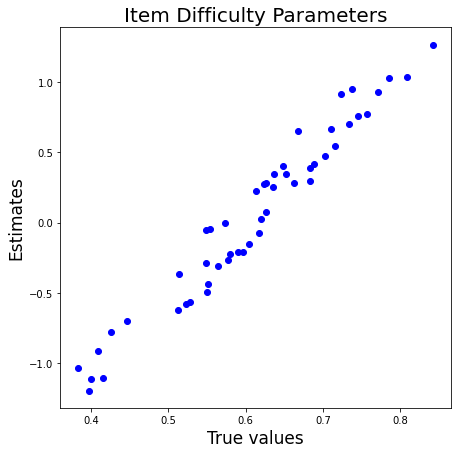
\includegraphics[width=.5\textwidth]{img/kt_irt/synth5_diff_est_lstm.png}
  \caption{Correlation between DKT-IRT estimates and true values of Synth5 item difficulty. SAKT-IRT produced similar results.}
  \label{fig:synth5_diff}
\end{figure}

A comparison between the output layer bias parameters and true item difficulty parameters is shown in Figure \ref{fig:synth5_diff}. This displays high correlation, and the trainable bias parameters in the output layer can be interpreted as approximations of the item difficulty parameters. Due to the available public dataset, there is no access to the true values of student abilities $\vect \Theta$.

\begin{figure}[h]
  \centering
  \minipage{.5\textwidth}
  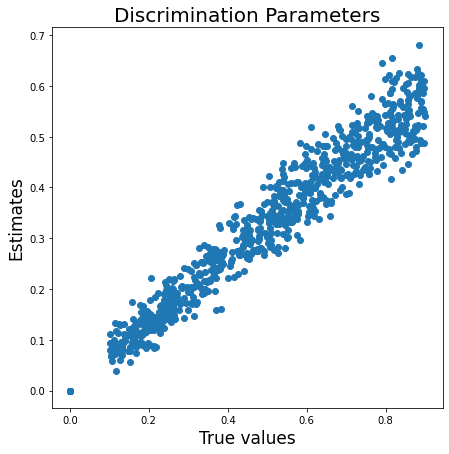
\includegraphics[width=.85\textwidth]{img/kt_irt/disc_est_attn2.png}
  \endminipage
  \minipage{.5\textwidth}
  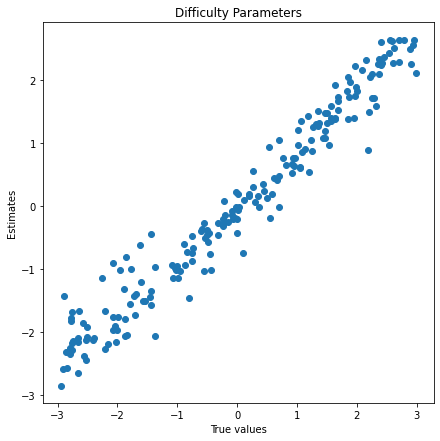
\includegraphics[width=.85\textwidth]{img/kt_irt/diff_attn_sim200.png}
  \endminipage
  \caption{Correlation between true and estimated Sim200 item discrimination parameters (left), and item difficulty parameters (right).}
  \label{fig:disc_diff_sim200}
\end{figure}

The parameter estimates can be directly compared to the true parameters in the Sim200 dataset. In Figure \ref{fig:disc_diff_sim200}, we can see the true values of item discrimination parameters $a_{ik}$ and item difficulty parameter. The correlation here is very high, and the estimates for item parameters are quite accurate. The student ability parameters $\theta_{jk}$ plotted against estimates given by SAKT-IRT at the final timestep in Figure \ref{fig:theta_sim200}. While there is a lot more noise in the student ability estimates, there is still significant correlation with the true values. 

It is important to note that the estimates to $\vect \Theta$ do not require any additional computation or transformation and are directly obtained from a hidden neural network layer. This is an advantage over other deep knowledge tracing methods, which only output the probability of answering items correctly and require other methods of quantifying knowledge concepts. Recall that while estimates to student ability are the neuron activation values at the skill layer from feeding forward a response sequence, the discrimination parameter estimates are the trained weights connecting the skill layer to the output layer, visualized in Figure \ref{fig:kt_irt_visual}.

\begin{figure}[h]
  \centering
  \includegraphics[width=.5\textwidth]{img/kt_irt/theta_est_attn2.png}
  \caption{Correlation between true and estimated student ability parameters at $t=L=200$ for the Sim200 dataset.}
  \label{fig:theta_sim200}
\end{figure}

\begin{figure}[h]
  \centering
  \includegraphics[width=.7\textwidth]{img/kt_irt/knowledge_trace_lstm_edited.png}\\
  \vspace{.5cm}
  \includegraphics[width=.7\textwidth]{img/kt_irt/knowledge_trace_attn_edited.png}
  \caption{Tracing a student's knowledge mastery with DKT-IRT (top) and SAKT-IRT (bottom) as they progress through the items of the Synthetic-5 dataset.}
  \label{fig:synth5_trace}
\end{figure}

The explcit representation of knowledge $\vect \Theta$ makes tracing student progress over time very convenient. For student $j$'s response sequence of length $L$, IRT-inspired knowledge tracing methods return a $K \times (L+1)$ matrix, where the entry $(k,t)$ gives the latent trait estimate to the $k$-th skill at time $t$, $\theta_{jkt}$. This is visualized in Figure \ref{fig:synth5_trace} on the Synth5 dataset. Notice how a correct response in a skill (filled-in circle) corresponds with a more green and less red skill value. Likewise, an incorrect response in a skill (hollow circle) corresponds with a more red skill or less green skill value. When comparing the knowledge tracing from DKT-IRT and SAKT-IRT, the DKT-IRT tracing is much more smooth as a student moves through the exam. This is likely because of the recurrent structure of an LSTM: the skill values at time $t$ are only directly related to the values at time $t-1$. The SAKT-IRT tracing graphic is much choppier, because the attention mechanism does not have smooth recurrent structure and instead maintains connections to all previous interactions.

\subsection{The Effect of Shuffled Responses}\label{sec:shuffle}
In Section \ref{sec:kt_data}, we mention that the orderings of each student's responses on the simulated datasets were randomly permuted. If all students answer all questions in the same order, then the IRT-inspired knowledge tracing method suffers greatly, particularly when viewing the item parameter estimates. This is due to how student knowledge $\vect \Theta$ is estimated initially at $t=0$, when no other information is provided to the model.

Consider the Sim200 dataset and assume that all students answer all items in the same order ($1, 2, \ldots,199,200$). At $t=0$, all students have the same estimate for their latent traits, $\hat{\theta}_{jk0} = s_{0k}^*$ for all $j$ as in Figure \ref{fig:kt_irt_visual} -- this is a poor estimate of student ability. This skill estimate is multiplied by the weight corresponding to a discrimination parameter of the first item, $w_{1k}q_{1k} = \hat a_{1k}$. 

Since every student answers item 1 first, the same value $s_{0k}^*$ is used in calculating $P(u_{1j} = 1)$ for all $j$. The innacuracy of $s_{0k}^*$ in all cases makes it difficult to estimate $a_{1k}$ -- the same is true for many items appearing early in the fixed response order. In Figure \ref{fig:no_shuffle}, we can compare the discrimination parameter estimates of items early versus late in the response order. Notice that the estimates are much more correlated with the true values for items towards the end of the sequence, since they have access to a more accurate estimate of each student's latent ability $\hat \theta_{jkt}$.

\begin{figure}[h]
  \centering
  \minipage{.5\textwidth}
  \includegraphics[width=.8\textwidth]{img/kt_irt/disc_est_no_shuffle_early.png}
  \endminipage
  \minipage{.5\textwidth}
  \includegraphics[width=.8\textwidth]{img/kt_irt/disc_est_no_shuffle_late.png}
  \endminipage
  \caption{Discrimination parameter estimates of items early in the response sequence (left) and items late in the response sequence (right) when all students answer items in the same order.}
  \label{fig:no_shuffle}
\end{figure}

\subsection{Using Attention to Learn Item-Skill Associations}
An advantage of other knowledge tracing methods such as DKT is that it does not require any expert annotation of the item-skill association. In other words, the only required data is the student response sequences, and not a $Q$-matrix. In the IRT-inspired knowledge tracing methods described in Chapter \ref{ch:kt_methods}, this $Q$-matrix is required to build the architecture used for the results reported in Section \ref{sec:kt_results}.

Multiple methods of discovering item-skill relationships from deep models have been proposed in the literature. For example, Piech et al. \cite{piech2015} proposes calculating the conditional influence between each item for this task. This involves finding the relative change that a correct response on item $i$ has on the probability of answering item $j$ correctly, computed by feeding the corresponding response sequences through DKT. In DKVMN \cite{zhang2017}, the correlation weights $\vect w_t$ from Equation \ref{eq:dkvmn_weight} are used to quantify the relationship between items and memory slots. A similar approach is used by Pandey et al. in SAKT \cite{pandey2019}, using the attention weight in Equation \ref{eq:attn_sakt} to relate each interaction in a response sequence.

We follow the framework of SAKT and use the attention mechanism to discover a $Q$-matrix. When using the SAKT-IRT architecture but removing the $Q$-matrix constraint, we arrive at a knowledge tracing framework that is nearly identical to SAKT. After training on the Synth5 dataset, we feed-forward a response sequence of a student answering all 50 items correctly After training on the Synth5 dataset, we feed-forward a response sequence of a student answering all 50 items correctly and calculated the correlation weights similar to Equation \ref{eq:attn_sakt}:
\begin{equation}
  \vect w_t = \text{softmax}\left(\frac{K \vect q_t}{\sqrt{d}} \right), \quad 0\leq t \leq 50
  \label{eq:q_cor_weights}
\end{equation}

We can arrange all correlation vectors $\vect w_t$ into a single matrix $C \in \R^{51 \times 51}$. A heatmap of $C$ is shown in Figure \ref{fig:attn_item_cor}. Note that the upper-right half of $C$ is all zero -- this is due to masking out future interactions (interaction $t$ cannot draw inferences from interaction $t+1$).
\begin{figure}[h]
  \centering
  \includegraphics[width=.65\textwidth]{img/kt_irt/synth5_attn_weights_no_ffn_axis2.png}
  \caption{Heatmap of the item correlation matrix $C$, where each row quantifies the relationship between an item and all previous items, starting in the top-left corner.}
  \label{fig:attn_item_cor}
\end{figure}
The sum of each row of $C$ is equal to 1, and each entry in row $i$ can be interpreted as the relevance between each previous interaction and item $i$. For example, item 42 draws some information from previous interactions 2, 5, 10, 19, and 24, seen in row 42. In a similar manner, item 4 is heavily relied upon for reference when querying interactions 21, 29, 30, 35, 40, and 41, seen in column 4.

The natural assumption is that items which are correlated by Equation \ref{eq:q_cor_weights} measure the same latent concept. To better visualize the item-skill association, we construct a weighted graph $G$, with each node representing an item and edge weights determined by the symmetric matrix $C + C^\top - \text{diag}(C)$. Using the NetworkX library for Python \cite{networkx}, we use a force-directed algorithm to visualize $G$ in 2-D space. This algorithm places node pairs with heavier weighted edges between them closer together \cite{fruchterman1991}, resulting in a clustering of items which are similar.

\begin{figure}[h]
  \centering
  \includegraphics[width=.55\textwidth]{img/kt_irt/synth5_clusters_no_ffn.png}
  \caption{Visualization of the graph $G$, showing a five clusters of items which correspond to the five concepts in the Synth5 dataset.}
  \label{fig:synth5_clusters}
\end{figure}
The graph $G$ is shown in Figure \ref{fig:synth5_clusters}. The different colors identify the true skill tag of each item -- this information was provided to neither the neural network nor the graph visualization algorithm. NetworkX was not even provided the number of skills, yet still arranges the nodes into five distinct clusters. Notice that all items of similar skill are clustered together, displaying that the correlation matrix $C$ in Figure \ref{fig:attn_item_cor} does in fact learn the item-skill associations. For example, items 42 and 4 are both found in clusters along with the items mentioned ealier which share larger values in $C$. The visualization of the graph $G$ can be used to build a $Q$-matrix for use in DKT-IRT or SAKT-IRT, as described in Section \ref{sec:kt_irt_methods}.

\section{Discussion}

\subsection{Future Extensions} \sideremark{TODO -- missing data framework, Q-matrix in attn calc}


\subsection{Concluding Remarks}
The connection between IRT and knowledge tracing presented in this work introduces a trade-off between accuracy and interpretability. Further work to increase AUC to the level of DKVMN while maintaining explainability is worth exploring. Though IRT-inspired knowledge tracing does require an expert to annotate the item-skill association $Q$-matrix while other methods do not, explicitly incorporating this domain knowledge greatly increases the ability to interpret a deep learning model. Further, most intelligent tutoring systems provide an item-skill tag, so availability of the $Q$-matrix is not an unreasonable assumption.

Our proposed method's ability to function as both a knowledge tracing model while also estimating item parameters gives it a unique interpretation rooted in Item Response Theory. This link with IRT is helpful in practice, because it provides an explicit and easy to obtain quantity for a student's latent abilities. The approximation of a student ability can be interpreted in the frame of IRT, as opposed to only a prediction of correctness for each item. This is a clear advantage that IRT-inspired knowledge tracing has over conventional non-interpretable deep learning methods in knowledge tracing.



% Part III
\chapter{Related Work}\label{ch:related_work}

How this type of technology can be used in other fields. Can talk about sports analytics paper and health sciences application.

% !Tex root = thesis.tex

% Appendices
\appendix \label{apdx}

%\chapter{Glossary of Notation}


\chapter{Artificial Neural Networks} \label{apdx:ann}
Artificial Neural Networks (ANN) are commonly understood to be complicated black box machine learning methods which produce high levels of accuracy, while sacrificing interpretability \cite{pattern_rec_book}. This assessment is true in part -- the end-to-end decision process of a trained neural network is very convoluted. But after zooming in to the inner workings of an ANN, each individual part is quite simple.

\section{Architecture}
Neural networks have a graph-like structure with vertices (nodes) and weighted edges. A basic feed-forward neural network (FFN) consists of an input layer, a number of hidden layers, and an output layer. A ``layer'' $l$ consists of $n_l$ nodes, and each node $i$ is connected to every node in the previous layer $l-1$ by a weighted edge. In this manner, the subgraph containing all nodes of layer $l-1$ and all nodes of layer $l$ can be seen as a complete bipartite graph $K_{n_{l-1}, n_l}$. A simple FFN is shown in Figure \ref{fig:ffn_example} which takes inputs with 10 features and classifies into three categories \cite{nn_svg}. For example, inputs could represent the weight, height, hair length, etc. of a pet, with the task of classifying the pet as a cat, dog, or bird \cite{neural_net}.

\sideremark{Edit this image with correct notation}
\begin{figure}[h]
  \centering
  \includegraphics[width=.85\textwidth]{img/ffn_visual.png}
  \caption{A basic FFN with input size $n_0 = 10$ and output size $n_3 = 3$, with two hidden layers of size $n_1 = 5$ and $n_2 = 6$.}
  \label{fig:ffn_example}
\end{figure}

While the architecture of a neural network can be described using the lens of graph theory, the inner workings are better described using basic linear algebra. Each layer acts as a function from $\R^{n_{l-1}}$ to $\R^{n_{l}}$. Specifically, this function is a linear transformation followed by a nonlinear re-scaling. For a given input vector $\vect x^* \in \R^{n_0}$ and its corresponding true label $\vect y^*$, the value in the first hidden layer is calculated as
\begin{equation}
  \vect a_1^* = f_1(W_1 \vect x^* + \vect b_1)
  \label{eq:hid_layer}
\end{equation}
where $W_1 \in \R^{n_1 \times n_0}$ and $\vect b_1 \in\R^{n_1}$ are the trainable \textit{weights} matrix and \textit{bias} vector. The notion of ``trainable'' parameters is explored further in Appendix \ref{apdx:backprop}. The value $\vect a_1^*$ is called the \textit{activation} value of the input $\vect x^*$ at hidden layer $l=1$. The non-decreasing function $f_1$ is called an \textit{activation function} which applies a (possibly) non-linear rescaling to the vector $\vect z_1^* = W_1 \vect x^* + \vect b_1 \in \R^{n_1}$ elementwise. Examples of different activation functions are given in Appendix \ref{apdx:activation_fcns}. Matrix notation can also be abandoned by writing the activation of the $i$-th node in layer $l=1$ as 
\begin{equation}
  a_{1,i}^* = f_1\left(b_{1,i} + \sum_{j=1}^{n_0} w_{ij}^1 \cdot x_j^* \right)
  \label{eq:element_activation}
\end{equation}
where $w_{ij}^1$ is the element in the $i$-th row and $j$-th column of $W_1$, the weight connecting the $j$-th node of layer $0$ to the $i$-th node of layer $1$.

The activation value of the input $\vect x^*$ at hidden layer $l=2$ and the output layer $l=3$ can similarly be computed as
\begin{equation}
  \begin{split}
    \vect a_2^* &= f_2(W_2 \vect a_1^* + \vect b_2) \\
    \hat{\vect y}^* &= \vect a_3^* = f_3(W_3 \vect a_2^* + \vect b_3)
  \end{split}
  \label{eq:ffn_comp}
\end{equation}
where the weights matrices $W_2 \in \R^{n_2 \times n_1}$ and $W_3 \in \R^{n_3 \times n_2}$ and bias vectors $\vect b_2 \in \R^{n_2}$ and $\vect b_3 \in \R^{n_3}$ are trainable. Before training, all trainable parameters are typically initialized randomly. The output value $\hat{\vect y}^*$ serves as the prediction for input $\vect x^*$. 

For classification, the true label is often a one-hot encoding, so the prediction $\hat{\vect y}^*$ should be a probability distribution each entry describes the certainty of model in classifying the input $\vect x^*$ as each possible class. Returning to the earlier example, an input with features pertaining to a cat has the true label $(1,0,0)$. An output prediction may give $(0.65, 0.32, 0.03)$, meaning that the neural network is $65\%$ sure that the input features are that of a cat, $32\%$ sure that the input is a dog, and $3\%$ sure that the input is a bird.

\section{Activation Functions} \label{apdx:activation_fcns}
The main purpose of activation functions is to rescale each layer so that every activation value falls in the same range. Doing multiple matrix multiplications in a row can easily cause values to become very large, and leading to overfitting and other complications \cite{sibi2013}. It can be helpful to use an activation function to map values to the range of $(0,1)$ because of the effect of the numbers $0$ and $1$ in multiplication, map to $(-1,1)$ to utilize positive and negative values, or map to $[0,\infty)$ to avoid negative values. 

Though custom activation functions can be defined and easily implemented, below are a few examples of popular activation functions used in neural networks \cite{tensorflow} \cite{keras_r}. Each of these are applied to a vector elementwise independently, except for the softmax function which maps an $n$-dimensional vector to an $n$-dimensional probability distribution.

\begin{equation}
  \text{Sigmoid: } \sigma(z) = \frac{1}{1 + e^{-z}} \quad \quad \R \to (0,1) 
  \label{eq:sigmoid_eqn}
\end{equation}
The sigmoid activation function has the form of the logistic curve and maps values to be between $0$ and $1$.

\begin{equation}
  \text{Hyperbolic tangent: } \tanh(z) = \frac{e^z - e^{-z}}{e^z + e^{-z}} \quad \quad \R \to (-1,1)
  \label{eq:tanh_eqn}
\end{equation}
Hyperbolic tangent has a similar curvature to that of the sigmoid, but maps values to between $-1$ and $1$. 

\begin{equation}
  \text{Rectified Linear Unit (ReLU): } \text{relu}(z) = \max\{0, z\} \quad \quad \R \to (0,\infty)
  \label{eq:relu_eqn}
\end{equation}
The ReLU function is often used to combat the ``learning slowdown'' problem that the sigmoid and $\tanh$ can face -- if an input $z_0$ is very large or very small, then the derivative $\frac{d\sigma}{dz} \Big|_{z=z_0}$ is very small, causing gradient descent iterations to improve slowly. THe derivative of the ReLU function is either exactly 0 or exactly 1, which helps speed up the training process.

\begin{equation}
  \text{Softmax: } \text{softmax}(\vect z)_i = \frac{e^{z_i}}{\sum_{j=1}^n e^{z_j}} \quad \quad \R^n \to \{P(x=i)\}_{i=1}^n
  \label{eq:softmax_eqn}
\end{equation}
When using the softmax activation function, the activation a single node is a function of the activation of all other nodes within the same layer. This is seen in the summation over $n$ nodes in Equation \ref{eq:softmax_eqn}. It is also straightforward to see that for any input, the sum of all $n$ nodes in the layer always adds up to exactly 1 -- so a softmax layer can be understood as a discrete probability distribution. This can be particularly useful in the output layer for a multi-class classification application.


\section{Optimization and Backpropagation}\label{apdx:backprop}
Figure \ref{fig:ffn_example} and Equations \ref{eq:hid_layer} and \ref{eq:ffn_comp} show that given an input $\vect x^*$, a feed-forward neural network can output a prediction $\hat{\vect y}^*$. We now turn to the way in which $\hat{\vect y}^*$ serves as a \textit{quality} prediction of the true value $\vect y^*$. The terminology ``train'' a neural network refers to finding optimal settings of the weights matrices $W_l$ and bias vectors $\vect b_l$ in each layer $l$ which minimize the error between predictions $\hat{\vect y}^*$ and true inputs $\vect y^*$. Such measures of error are called \textit{loss functions}.

Though there are many candidates for loss functions such as cross-entropy (see Equation \ref{eq:cross_entropy}) or hinge loss \cite{gentile1998}, consider the simple mean squared-error loss function
\begin{equation}
  \mathcal{L}(\vect y, \hat{\vect y}) = ||\vect y - \hat{\vect y}||_2^2 = \frac{1}{K} \sum_{k=1}^K (y_k - \hat{y}_k)^2
  \label{eq:mse_loss}
\end{equation}
where $K$ is the dimension of the target (e.g. the number of output nodes).

Recall that if an input (or set of inputs) $\vect x^*$ is fixed, then the prediction outputted by the neural network is a function of the weights and biases $W_l$ and $\vect b_l$. As such, we can compute partial derivatives of $\mathcal{L}$ with respect to each trainable parameter and use a gradient descent algorithm to minimize Equation \ref{eq:mse_loss}.

Though deep neural networks can have thousands, millions, or billions of parameters \cite{gpt3}, calculating gradients remains feasible because of the backpropagation algorithm \cite{rojas1996}. While obtaining predictions from a neural networks works in a left-to-right fashion ($\vect a_3$ depends on $\vect a_2$ depends on $\vect a_1$ depends on $\vect x$), gradient calculations are computed right-to-left. This is due to the role of the chain rule.

First consider calculating the partial derivative of a particular weight in the final layer $w_{ij}^3$. Denote the input to an activation function at layer $l$ as $\vect z_l = W_l \vect a_{l-1} + b_l$ so that $\vect a_l = f_l(\vect z_l)$. Using Equation \ref{eq:ffn_comp}, we can write
\begin{equation}
  \frac{\partial \mathcal{L(\vect y, \vect a_3)}}{\partial w_{ij}^3} = \frac{\partial \mathcal{L}(\vect y, \vect a_3)}{\partial a_{3,i}} \cdot \frac{\partial a_{3,i}}{\partial z_{3,i}} \cdot \frac{\partial z_{3,i}}{\partial w_{ij}^3} = \frac{\partial \mathcal{L}(\vect y, \vect a_3)}{\partial a_{3,i}} \cdot f_3'(z_{3,i}) \cdot a_{2,j} 
  \label{eq:chain_rule}
\end{equation}
Now consider the change in loss with respect to a trainable parameter in the second-to-last layer. Choose a weight $w_{jk}^2$ whose right endpoint is the same node as the left endpoint of $w_{ij}^3$ used in Equation \ref{eq:chain_rule}. We have
\begin{equation}
  \begin{split}
    \frac{\partial \mathcal{L}(\vect y, \vect a_3)}{\partial w_{kj}^2} &= \sum_{i=1}^K \left(\frac{\partial \mathcal{L}(\vect y, \vect a_3)}{\partial a_{3,i}} \cdot \frac{\partial a_{3,i}}{\partial z_{3,i}} \cdot \frac{\partial z_{3,i}}{\partial a_{2,j}}\right) \cdot \frac{\partial a_{2,j}}{\partial z_{2,j}} \cdot \frac{\partial z_{2,j}}{\partial w_{jk}^2} \\
    &= \sum_{i=1}^K \left(\frac{\partial \mathcal{L}(\vect y, \vect a_3)}{\partial a_{3,i}} \cdot f_3'(z_{3,i}) \cdot w_{ij}^3 \right) \cdot f_2'(z_{2,j}) \cdot a_{1,k}
\end{split}
  \label{eq:chain_rule2}
\end{equation}

Notice how in Equation \ref{eq:chain_rule2}, information first calculated in Equation \ref{eq:chain_rule} is re-used. Particularly, the partial derivative of a parameter found in layer $l$ is a sum of partial derivatives of values found in layer $l+1$. In this sense, the backpropagation algorithm works right-to-left; first calculating values in layer $L$ that will later be used in all layers $l<L$.

After the gradient of $\mathcal{L}$ is found using backpropagation, a gradient descent update is performed for an input $\vect x$:
\begin{equation}
  \vect \Lambda_{t+1} \gets \vect \Lambda_{t} - \eta \nabla_{\vect \Lambda} \mathcal{L}(\vect y, \hat{\vect y})
  \label{eq:grad_update}
\end{equation}
where $\vect \Lambda$ is a vector containing all trainable parameters $W_l$ and $\vect b_l$ and $\eta$ is the learning rate hyperparameter \cite{ruder2017}. This process is repeated with different inputs from the training set $\vect x$. \sideremark{TODO: could give more on SGD, adam, etc}


\chapter{\textbf{ML2Pvae} Package Details} \label{apdx:software}
In this section, we provide a tutorial of the \textbf{ML2Pvae} software package for R. Functions and data which are exported by the package are listed in {\color{blue}\verb!blue!}. This tutorial uses a simulated dataset which is accessible through the package, including:
\begin{itemize}
  \item A $Q$-matrix ({\color{blue}\verb!q_matrix!}) relating $n = 30$ items to $K = 3$ latent skills
  \item A covariance matrix ({\color{blue}\verb!correlation_matrix!}) detailing the correlations between the latent skills
  \item A set of $N = 5,000$ binary responses ({\color{blue}\verb!responses!}) to $n = 30$ items, generated by the ML2P model with true parameters:
    \begin{itemize}
      \item $\vect \Theta_j \in \R^3$, $1\leq j \leq 5,000$ ({\color{blue}\verb!theta_true!})
      \item $\vect a_i \in \R^3$, $1\leq i \leq 30$ ({\color{blue}\verb!disc_true!})
      \item $b_i\in \R$, $1\leq i \leq 30$ ({\color{blue}\verb!diff_true!}) 
    \end{itemize}
\end{itemize}

The \textbf{ML2Pvae} package has five easy-to-use functions to assist in building, training, and evaluating ML2P-VAE models. The functions {\color{blue}\verb!build_vae_independent()!} and {\color{blue}\verb!build_vae_correlated()!} construct a modified VAE architecture as specified by the user. The former assumes that the latent traits are independent ($\vect \Theta \sim \mathcal{N}(0,I)$), and the latter assumes knowledge of correlated latent traits ($\vect \Theta \sim \mathcal{N}(\vect \mu, \Sigma)$), as described in Section \ref{sec:cov}.

To train a VAE on a dataset, the function {\color{blue}\verb!train_model()!} can be used. After the model has been fitted, the function {\color{blue}\verb!get_item_parameter_estimates()!} grabs the relevant trainable weights from the decoder which serve as estimates of $\vect a_i$ and $b_i$. The function {\color{blue}\verb!get_ability_parameter_estimates()!} feeds student responses through the encoder to obtain estimates to $\vect \Theta_j$.

The functionality of \textbf{ML2Pvae} is displayed below. Note that while the neural network models are created with Tensorflow and Keras \cite{keras_r} inside of \textbf{ML2Pvae}, those packages are not employed by the user. This is by design to make the ML2P-VAE method accessible to IRT researchers who may not have knowledge of neural networks. Further explanation and documentation for \textbf{ML2Pvae} can be found at {\color{violet}\href{https://cran.r-project.org/web/packages/ML2Pvae}{https://cran.r-project.org/web/packages/ML2Pvae}}. Source code of the software is found at {\color{violet}\href{https://github.com/converseg/ML2Pvae}{https://github.com/converseg/ML2Pvae}}.

\section{Software Tutorial}
\vspace{.5cm}

%\lstset{language=R, keywords={}, otherkeywords={build\_vae\_independent, build\_vae\_correlated, train\_model, get\_item\_parameter\_estimates, get\_ability\_parameter\_estimates, responses, q\_matrix, correlation\_matrix, disc\_true, diff\_true, theta\_true}}
\lstinputlisting{ml2pvae_tutorial.R}
\begin{figure}[h]
  \centering
  \includegraphics[width=.95\textwidth]{img/ml2pvae_tutorial_plots.png}
  \caption{Correlation plots of IRT parameter estimates produced by the above code tutorial.}
  \label{fig:tutorial_plots}
\end{figure}


%\chapter{Details on Related Works}





% this command includes the entire bib file in the
% references section, whether the entry has been
% cited in the paper or not
%
%\nocite{*}

\biblio{thesis}



%\bibliographystyle{plain}
%\bibliography{thesis} % I guess this makes citations work?

%\singlespacing

\end{document}
